
%+----------------------------------------------------------------------------+
%| SLIDES: Phd colloquium
%| Contents:	- 45 minutes (extimated duration 3 minutes per slide )
%|
%| Author: Antonio miti
%| Place: Leuven, April 2021
%+----------------------------------------------------------------------------+


%- HandOut Flag -----------------------------------------------------------------------------------------
\newif\ifHandout
%\Handouttrue  %uncomment for the printable version


%- D0cum3nt ----------------------------------------------------------------------------------------------
\ifHandout
	\documentclass[handout,10pt]{beamer}   
	\setbeameroption{show notes} %print notes   
\else
	\documentclass[10pt]{beamer}
\fi



%- Packages ----------------------------------------------------------------------------------------------
\usepackage{custom-style}
\usepackage{array}
\usepackage{pbox}

%--Beamer Style-----------------------------------------------------------------------------------------------
\usetheme{toninus}
\usepackage{animate}
\usetikzlibrary{positioning, arrows}
\usetikzlibrary{shapes,decorations}
\usetikzlibrary{backgrounds}
  \tikzset{
    invisible/.style={opacity=0},
    visible on/.style={alt=#1{}{invisible}},
    alt/.code args={<#1>#2#3}{%
      \alt<#1>{\pgfkeysalso{#2}}{\pgfkeysalso{#3}} % \pgfkeysalso doesn't change the path
    },
  }



%- T1tle P4g3 -------------------------------------------------------------------------------------------
\title{What is ... \\ Geometric Mechanics} 
\subtitle{\href{ttps://set.kuleuven.be/phd/sap/dualjoint/public}{PhD Colloquim}}
\author[AMM]{\href{https://dmf.unicatt.it/miti/}{Antonio Michele Miti}}
\institute[UCSC and KU Leuven]{
  \begin{tabular}[h]{ccc}
      Università Cattolica del Sacro Cuore & $\qquad$ & KU Leuven \\
      Brescia, Italy & & Leuven, Belgium \\
      \href{https://dipartimenti.unicatt.it/dmf-home?rdeLocaleAttr=it}{
\includegraphics[width=3.5cm]{./Logos/UnicattBS-logo}} & & 
      \href{https://wis.kuleuven.be/english}{
\includegraphics[width=4cm]{./Logos/KULeuven_logo}}
  \end{tabular}      
}
\date[PublicDefence_21] % (optional, should be abbreviation of conference name)
{	
	\href{https://scuoledidottorato.unicatt.it/phdschools/science-home}{International Doctoral Programme in Science } \\
	{\vskip 1ex}
	KU Leuven, April 28, 2021
}





\newcommand{\thankyouslide}[0]{
	\ifHandout

	\else
	\addtocounter{framenumber}{-1}
	\begin{frame}{}
	\label{frame:thankyouslide}
		\vfill
	  \centering 
	  {\Huge\color{red} 
	  \emph{Thank you for your attention!}}
		\vfill
		%
		\centering
		\fbox{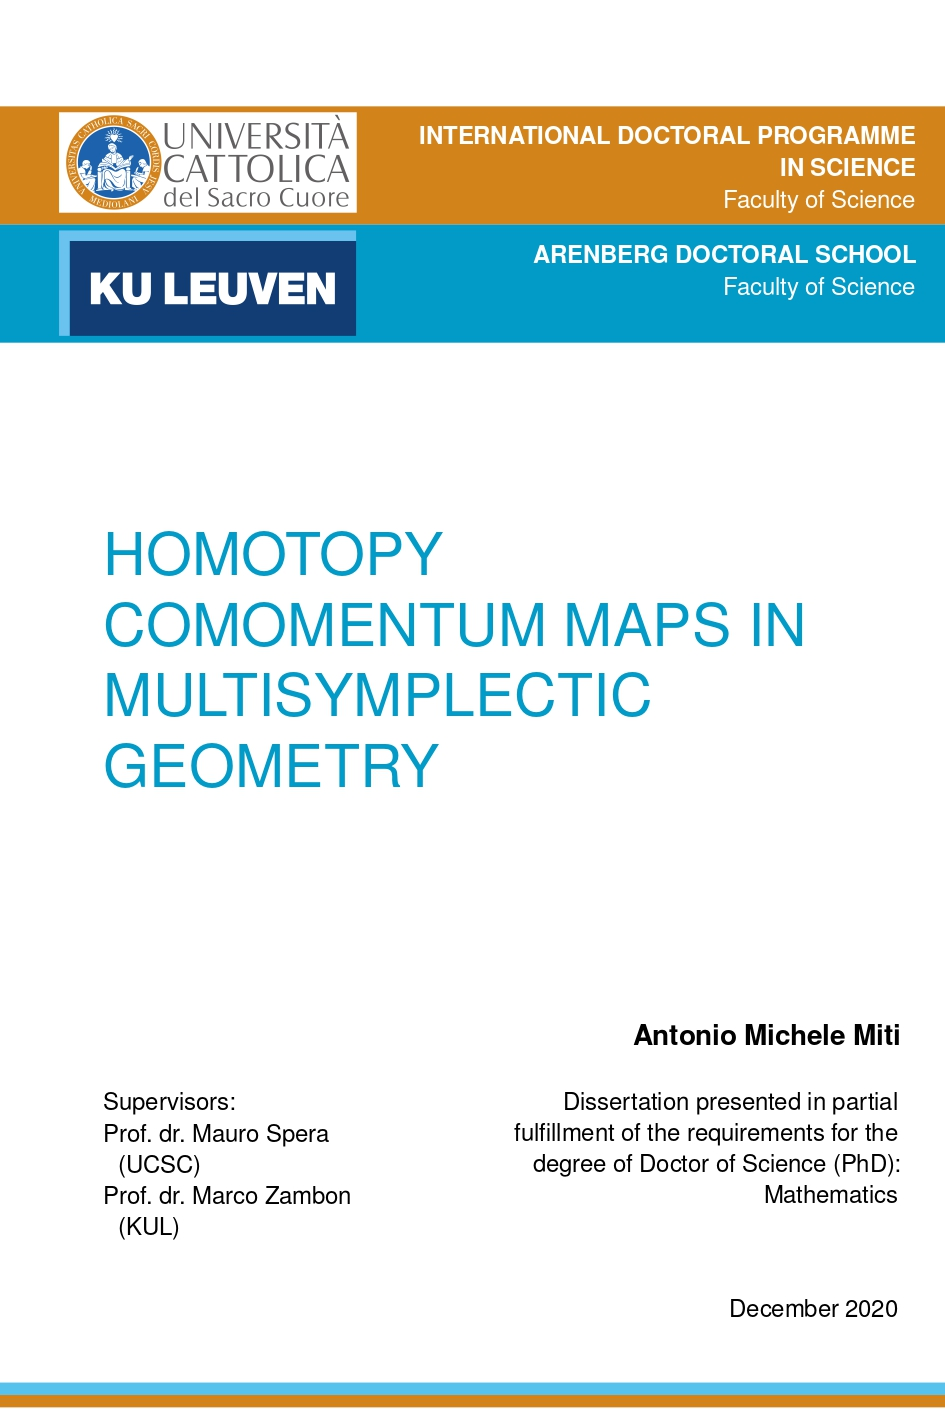
\includegraphics[width=.4\textwidth]{Pictures/thesis-cover}}
	\end{frame}
	\note[itemize]{
		\item
	}
	\fi
}






%---------------------------------------------------------------------------------------------------------------------------------------------------
%- D0cum3nt ----------------------------------------------------------------------------------------------------------------------------------
\begin{document}
%-------------------------------------------------------------------------------------------------------------------------------------------------
\begin{frame}  % Alternative: \maketitle outside of frame
	\titlepage
	\ifHandout
		\tikz[overlay,remember picture]
		{
	    	%	\node at ($(current page.west)+(1.5,0)$) [rotate=90] {\Huge\textcolor{gray}{\today}};
	    	\node[        
	    		draw,
	    		shape border rotate=90,
			isosceles triangle,
			isosceles triangle apex angle=90,
			fill=yellow]
	        		at ($(current page.north east)-(1,1)$) [rotate=-45] {\textcolor{red}{Handout version}};
		}
	\fi
	\end{frame}
	\addtocounter{framenumber}{-1}
\note{
	%Abstract?
	%\textbf{\underline{OUTLINE}}:
	%\tableofcontents
	\textbf{Abstract:}
	\\
    Geometric mechanics is a branch of mathematics applying differential geometry methods to many areas of mechanics, from the dynamics of point-particles to continuous media.
	\\
    In this talk, we review the three cornerstones of this discipline - phase space, observables and symmetries- focussing on the centrality of the notion of symplectic forms. If time permits we will also discuss a possible generalization of the latter notion, named multisymplectic structure, that can be useful to encode mechanical systems with infinite degrees of freedom in a finite-dimensional setting.
	\\
    The crucial message is that, just as geometry provide an intuition of how mechanical systems evolve, mechanics provides a context for interpreting many abstract differential geometry objects.	
	
}
%---------------------------------------------------------------------------------------------------------------------------------------------------





%-------------------------------------------------------------------------------------------------------------------------------------------------
\section{Introduction}
%-------------------------------------------------------------------------------------------------------------------------------------------------
	%- HandOut Flag -----------------------------------------------------------------------------------------
\newif\ifHandout

%- D0cum3nt ----------------------------------------------------------------------------------------------
\documentclass[beamer,10pt]{standalone}   
%\documentclass[beamer,10pt,handout]{standalone}  \Handouttrue  

%- HandOut Flag -----------------------------------------------------------------------------------------
\ifHandout
	\setbeameroption{show notes} %print notes   
\fi

	
%- Packages ----------------------------------------------------------------------------------------------
\usepackage{custom-style}
\usetikzlibrary{positioning}
\usepackage{multicol}


%--Beamer Style-----------------------------------------------------------------------------------------------
\usetheme{toninus}
\usepackage{animate}
\usetikzlibrary{positioning, arrows}
\usetikzlibrary{shapes}

\begin{document}
%-------------------------------------------------------------------------------------------------------------------------------------------------
\begin{frame}{Introduction}
	\begin{columns}[]
	\begin{column}{0.55\textwidth}
		PhD colloquium:
		\\
		i.e.~
		\emph{a talk inspired by my doctoral project}

	\vspace{1em}

	\begin{itemize}
		\item<2-> \underline{Thesis}: focus on certain \emph{higher generalizations} in \emph{ symplectic geometry}.
		\item<3-> \underline{Talk}: focus on \emph{motivations} rather than details.
	\end{itemize}	



	\end{column}
	\begin{column}{0.4\textwidth}
		\onslide<2->{
			\fbox{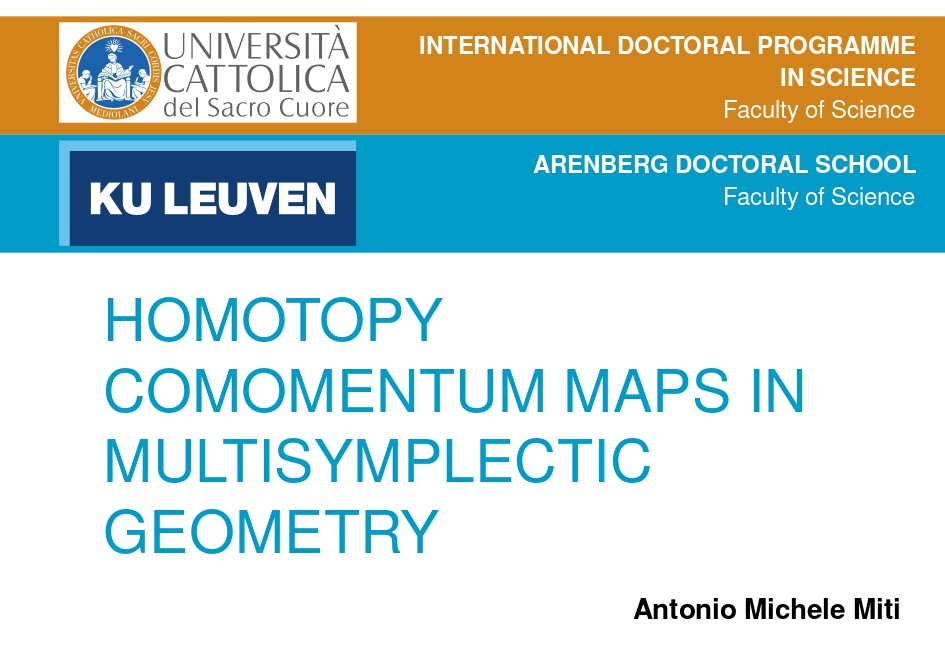
\includegraphics[width=.9\textwidth]{Pictures/thesis-zoom}}
		}
	\end{column}
	\end{columns}

	\vfill

	\vfill
	\begin{columns}[]
	\begin{column}{0.35\textwidth}
		\onslide<4->{
			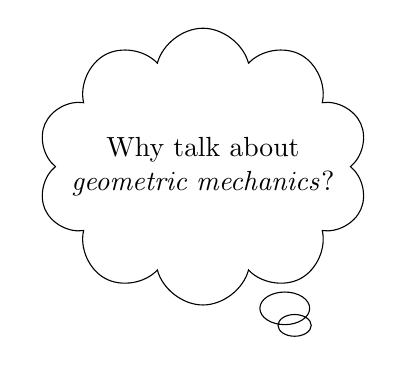
\begin{tikzpicture}
				\node [draw,cloud callout, minimum height=10em,minimum width=12em] (L1) {};
				\node [text width=12em,text centered] (L2) {Why talk about \\ \emph{geometric mechanics}?};
			\end{tikzpicture}
		}
	\end{column}
	\begin{column}{0.65\textwidth}
		\onslide<5->{
			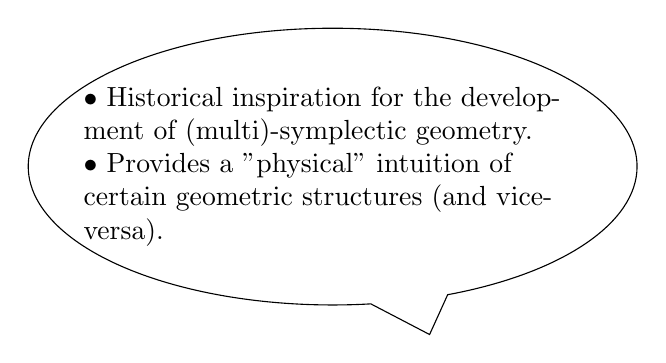
\begin{tikzpicture}
				\node [draw,ellipse callout, minimum height=10em,minimum width=22em] (L1) {};
				\node [text width=18em] (L2) 
					{
						$\bullet$ Historical inspiration for the development of (multi)-symplectic geometry.
						\\
						$\bullet$ Provides a "physical" intuition of certain geometric structures (and vice-versa).
					};
			\end{tikzpicture}
		}
	\end{column}
	\end{columns}



\end{frame}
\note[itemize]{
	\item
}
%-------------------------------------------------------------------------------------------------------------------------------------------------

\outline

\subsection{Geometry \& Physics}
%-------------------------------------------------------------------------------------------------------------------------------------------------
\begin{frame}[t,fragile]{What is... mechanics?}
	\begin{center}
		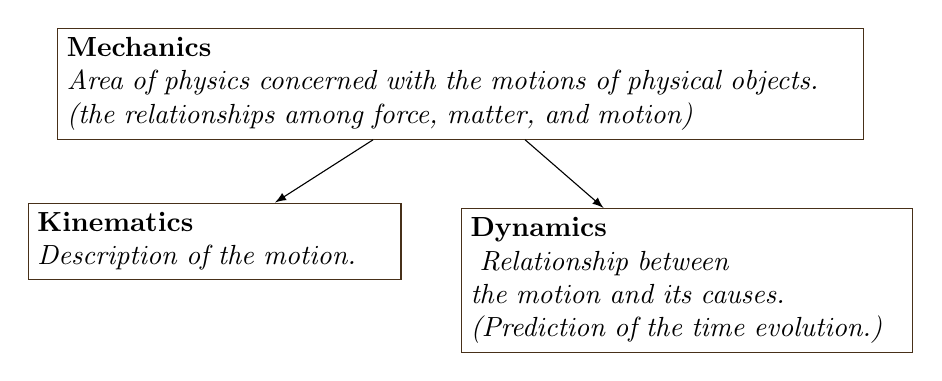
\begin{tikzpicture}
		 	\node[draw=orange!20!black!90,right,text width=10cm] (s1) at (0,0)
		    {
				{\bf Mechanics} \\
				\emph{Area of physics concerned with the motions of physical objects.\\
				(the relationships among force, matter, and motion)}		            
		     }; 
 			\node[draw=orange!20!black!90,text width=4.5cm] (t1) at (2cm,-2cm)
    		{
		   		{\bf Kinematics}
		   		\\ \emph{Description of the motion.}
	        };	
 			\node[draw=orange!20!black!90,text width=5.5cm] (t2) at (8cm,-2.5cm)
    			{
		    		{\bf Dynamics} \\
		   			\emph{ Relationship between\\ the motion and its causes.\\ (Prediction of the time evolution.)}
	        };
	        \draw[-latex] (s1) -- (t1);
        	\draw[-latex] (s1) -- (t2);
		\end{tikzpicture}
	\end{center}

	\vfill
	\begin{columns}
    	\begin{column}{.33\textwidth}
	   		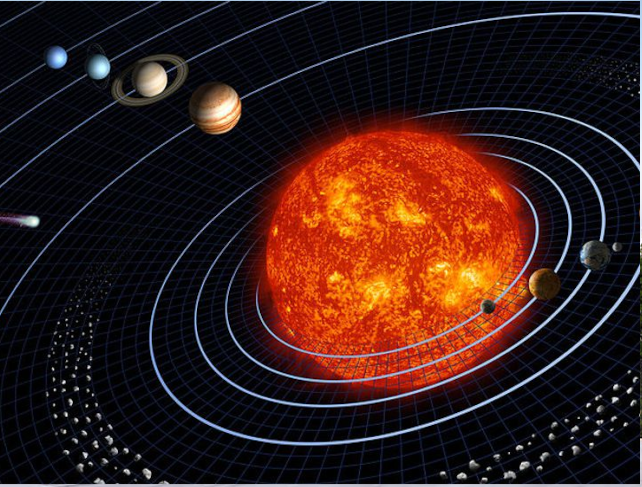
\includegraphics[width=\textwidth]{Pictures/solar} 	
		\end{column}
    	\begin{column}{.33\textwidth}
	   		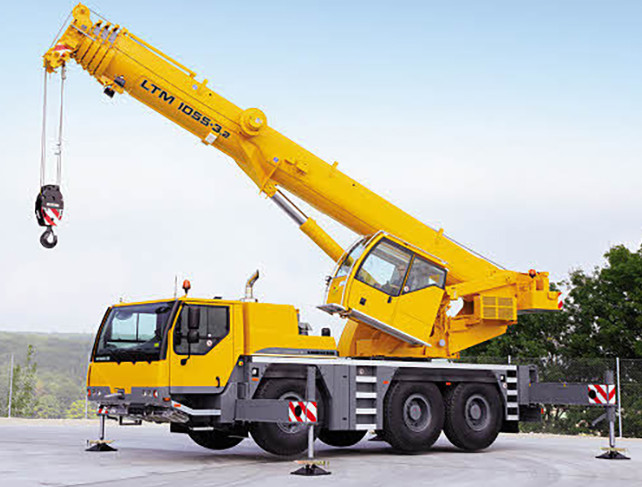
\includegraphics[width=\textwidth]{Pictures/autogru-liebherr} 	
		\end{column}
    	\begin{column}{.33\textwidth}
	   		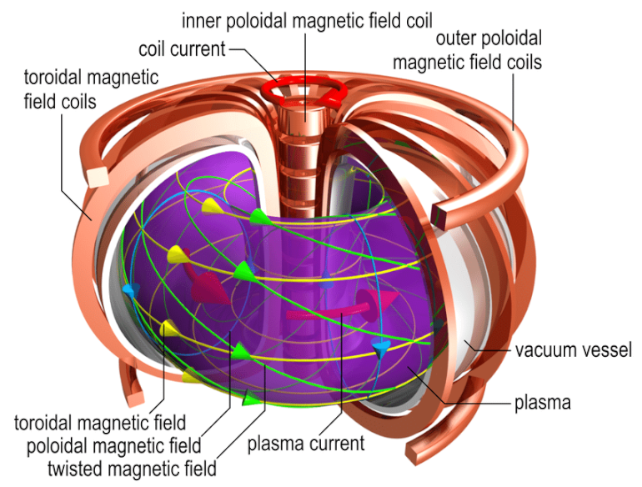
\includegraphics[width=\textwidth]{Pictures/plasma} 	
		\end{column}
	\end{columns}
\end{frame}
\note[itemize]{
	\item
}
%-------------------------------------------------------------------------------------------------------------------------------------------------

%-------------------------------------------------------------------------------------------------------------------------------------------------
\begin{frame}[t]{How does Geometry gets into Physics?}
	%
	\begin{block}{Trivial answer:}
		It appears in describing the "physical space" in which all "physical systems" are embedded.
	\end{block}
	\vfill

  	\begin{columns}<2->
  		\hfill
    	\begin{column}{.6\textwidth}
    		\begin{block}{Historical fact:}
				Measuring "Earth" is one of the oldest problem in mathematics.
			\end{block}
    	\end{column}
    	\begin{column}{.3\textwidth}
			\center
			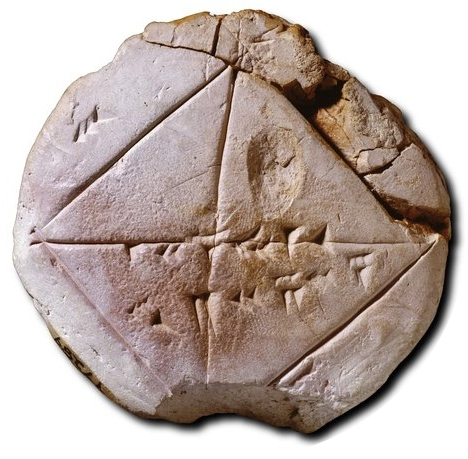
\includegraphics[width=0.5\textwidth]{Pictures/babylon-tablet} 		
    	\end{column}
    \end{columns}
    %
    \vspace*{-.5em}    
  	\begin{columns}<3->
  		\hfill
    	\begin{column}{.3\textwidth}
    		\center
			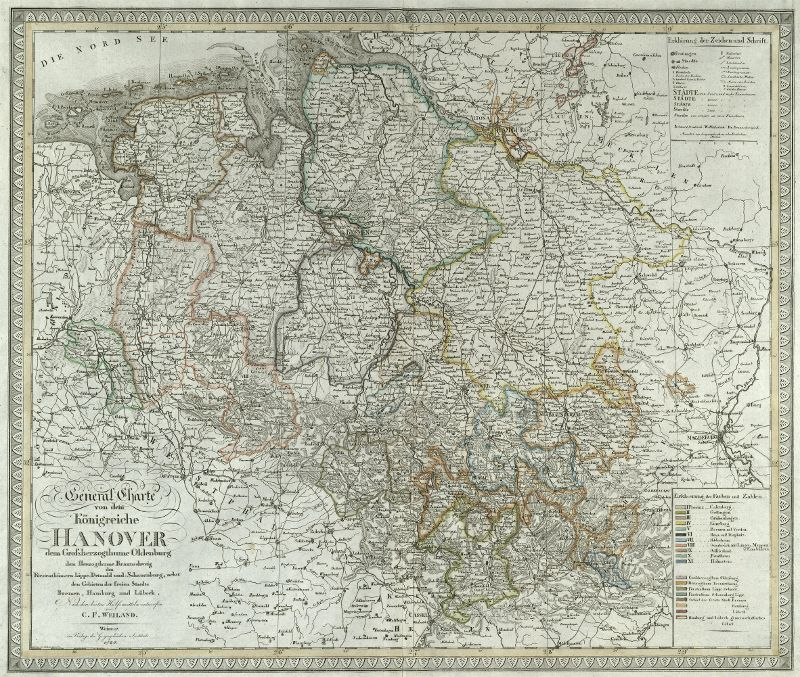
\includegraphics[width=0.8\textwidth]{Pictures/hannover-map} 		
    	\end{column}
    	\begin{column}{.6\textwidth}
				Also modern (intrinsic) differential geometry stemmed from cartography!
				\\
				\small (a cartographic survey of the Kingdom of Hanover commissioned to Carl Friederich Gauss in 1828.)	    			
		\end{column}
    \end{columns}    
    
    
	\vfill
	\begin{alertblock}<4->{There is much more!}
		Geometry provides a powerful language to encode deep properties of physics encompassing a huge variety of mechanical systems.
	\end{alertblock}
\end{frame}
\note[itemize]{
	\item Three fundamentals concepts: Space, Body (system), Displacement.
	\item Nevertheless, the problem of measuring "Earth" is one of the oldest problem in mathematics (see \url{https://en.wikipedia.org/wiki/YBC_7289})
	\item YBC 7289 is a Babylonian clay tablet notable for containing an accurate sexagesimal approximation to the square root of 2, the length of the diagonal of a unit square. 
	\item Nel 1818 fu chiesto a Gauss di compiere la rilevazione geodetica del Regno di Hannover, associandola ai precedenti rilevamenti effettuati in Danimarca.
La cartografia dell'Hannover portò Gauss a sviluppare la geometria differenziale insieme alle potenzialità della geometria non euclidea.
}
%-------------------------------------------------------------------------------------------------------------------------------------------------

%-------------------------------------------------------------------------------------------------------------------------------------------------
\subsection{Geometric mechanics in a nutshell}
\begin{frame}{What we mean by: \emph{Geometric mechanics}? (1)}
	\alert{"Geometric mechanics" is not a completely standard (widely accepted) term.} \\
	It needs some clarification...
	\vfill
	\pause
	The idea of intermarrying geometry with mechanics has a noble father...
	\begin{columns}[T]
		\begin{column}{.4\textwidth}
			\center
			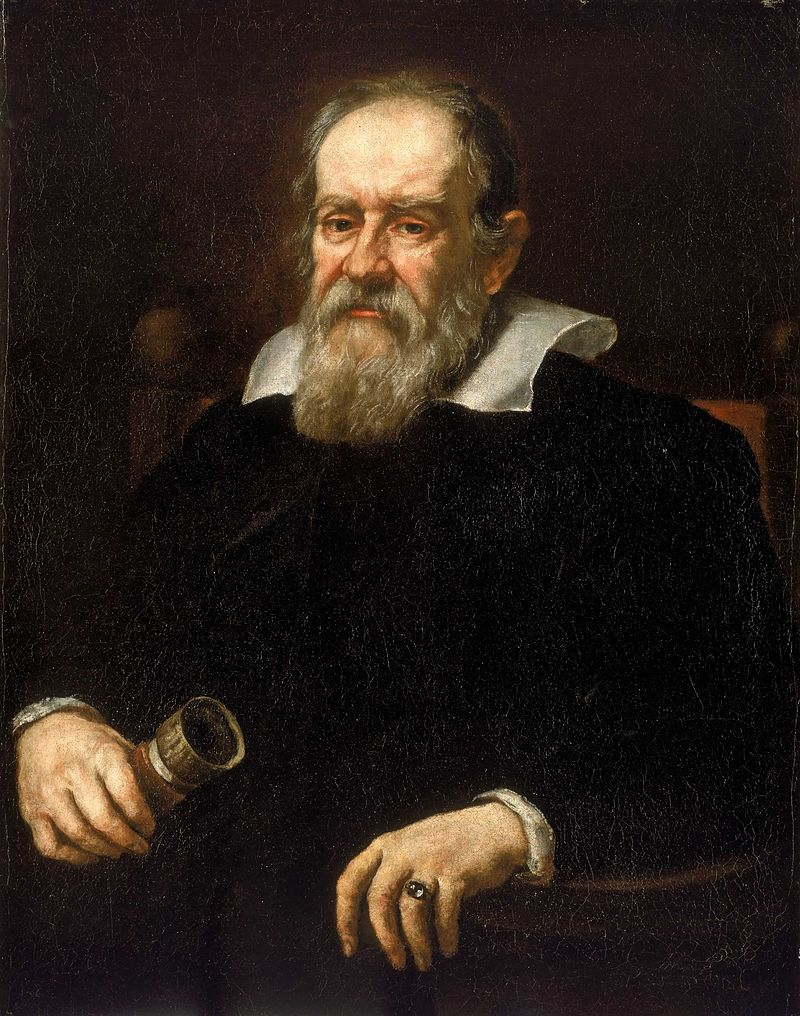
\includegraphics[width=0.8\textwidth]{Pictures/FFat/Galileo} 
		\end{column}
		\begin{column}{.6\textwidth}
			\only<2>{
			\begin{quotation}
			{\footnotesize 
				«La filosofia è scritta in questo grandissimo libro che continuamente ci sta aperto innanzi a gli occhi (io dico {\bf l'universo}), ma non si può intendere se prima non s'impara a intender la lingua, e conoscer i caratteri, ne' quali è scritto. 
				Egli {\bf è scritto in lingua matematica, e i caratteri son triangoli, cerchi, ed altre figure geometriche}, senza i quali mezzi è impossibile a intenderne umanamente parola; senza questi è un aggirarsi vanamente per un oscuro laberinto.»
			}
			\end{quotation}
			}
			\only<3->{		
			\begin{quotation}
			{\footnotesize 
				«Philosophy {\bf [nature]} is written in that great book which ever is before our eyes -- I mean the universe -- but we cannot understand it if we do not first learn the language and grasp the symbols in which it is written. 
				The book {\bf is written in mathematical language, and the symbols are triangles, circles and other geometrical figures}, without whose help it is impossible to comprehend a single word of it; without which one wanders in vain through a dark labyrinth.»		
			}
			\end{quotation}	
			}
			(Galileo Galilei, Il Saggiatore, 1623)	
		\end{column}	
	\end{columns}	
\end{frame}
\note[itemize]{
	\item Praticamente l'idea è vecchia quanto la scienza.f
}
%-------------------------------------------------------------------------------------------------------------------------------------------------


%-------------------------------------------------------------------------------------------------------------------------------------------------
\begin{frame}{What we mean by: \emph{Geometric mechanics}? (2)}
	What we mean \underline{here} is:
	\\
	the modern discipline originated in the 60s by the work of these mathematicians%gentlemen
	
	\vfill
	\begin{columns}[T]
		\begin{column}{.2\textwidth}
			\center
			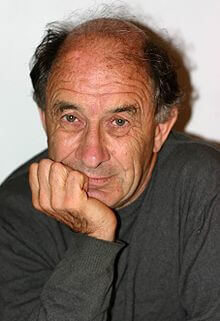
\includegraphics[width=0.8\textwidth]{Pictures/FFat/arnold}
			Vladimir \\ 
			Arnold
		\end{column}
		\begin{column}{.2\textwidth}
			\center
			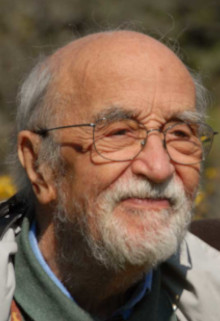
\includegraphics[width=0.8\textwidth]{Pictures/FFat/souriau} 
			Jean-Marie \\			
			Souriau
		\end{column}
		\begin{column}{.2\textwidth}
			\center
			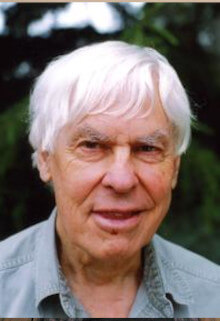
\includegraphics[width=0.8\textwidth]{Pictures/FFat/smale}
			Stephen \\
			Smale
		\end{column}
		\begin{column}{.2\textwidth}
			\center
			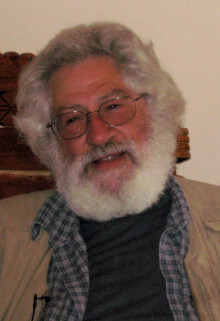
\includegraphics[width=0.8\textwidth]{Pictures/FFat/abraham} 
			Ralph \\			
			Abraham
		\end{column}
		\begin{column}{.2\textwidth}
			\center
			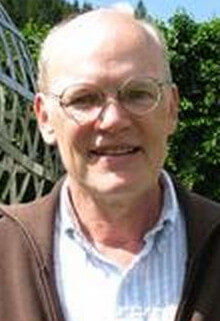
\includegraphics[width=0.8\textwidth]{Pictures/FFat/marsden} 
			Jerrold \\
			Marsden
		\end{column}		
	\end{columns}	

	\pause
	\vfill
	\begin{block}<1->{Introduced as a branch of \emph{(applied) Mathematics}}
			Employs modern (differential) geometry to the description of dynamical systems.	
	\end{block}


\end{frame}
\note[itemize]{
	\item %\href{https://en.wikipedia.org/wiki/Geometric_mechanics#History}{wiki}
		Arnold's fundamental work showed that Euler's equations for the free rigid body are the equations for geodesic flow on the rotation group SO(3) and carried this geometric insight over to the dynamics of ideal fluids, where the rotation group is replaced by the group of volume-preserving diffeomorphisms. 
	\item Smale's paper on Topology and Mechanics investigates the conserved quantities arising from Noether's theorem when a Lie group of symmetries acts on a mechanical system, and defines what is now called the momentum map (which Smale calls angular momentum), and he raises questions about the topology of the energy-momentum level surfaces and the effect on the dynamics. 
	\item Souriau also considered the conserved quantities arising from the action of a group of symmetries, but he concentrates more on the geometric structures involved (for example the equivariance properties of this momentum for a wide class of symmetries), and less on questions of dynamics.
	\item These ideas leads to the seminal book: \emph{Foundations of Mechanics} by Abraham and Marsden (1978).
	\item 		{physical è un po' restrittivo, diciamo sistemi che evolvono?}	
		{dynamical systems: non solo meccanica classica non relativistica non quantistica!}

}
%-------------------------------------------------------------------------------------------------------------------------------------------------

%-------------------------------------------------------------------------------------------------------------------------------------------------
\begin{frame}[t]{What is... \emph{Geometric Mechanics?}}
		\begin{block}{As an approach to \emph{Rational Mechanics}:}
			\begin{itemize}
				\item \textbf{Key idea:} make use of geometry to completely encode a physical system's mechanical properties regardless of the coordinate system employed.
				\item \textbf{The goal:} reconstruction of the physical observable quantities of interest from this abstract mathematical setting.
				\item \textbf{Advantages:} formalize the system's relevant structure in order to:
					\begin{itemize}
						\item[-] simplify the analytical or numerical solution of motion equations;
						\item[-] derive its quantum or relativistic counterpart.		
					\end{itemize}									
			\end{itemize}
		\end{block}
		%
		\vfill
		\pause
		\begin{block}{Some direct applications:}
			\vspace{-0.5em}
			\begin{columns}
		    	\begin{column}{.45\textwidth}
					\begin{itemize}
						\item[-] Theoretical chemistry
						\item[-] Control theory
						\item[-] Image processing
					\end{itemize}
				\end{column}
		    	\begin{column}{.45\textwidth}
					\begin{itemize}
						\item[-] Mathematical finance
						\item[-] Earth sciences
						\item[-] Robotics
					\end{itemize}
				\end{column}
			\end{columns}
		\end{block}
		\vfill
		\pause
		\begin{block}{Three cornerstones of geometric mechanics}
	\begin{center}
		%\scalebox{.8}{%
		{
		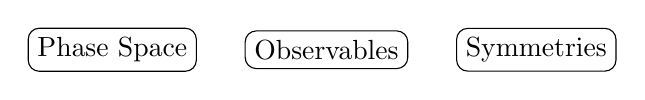
\begin{tikzpicture}[>=stealth,every node/.style={shape=rectangle,draw,rounded corners},node distance=0.05\linewidth,]
	    % create the nodes
		    \node (a1) {Phase Space};
		    \node (a2)[right =of a1] {Observables};
		    \node (a3)[right =of a2] {Symmetries};
		\end{tikzpicture}
%				\node [text width=0.6\linewidth, rectangle,draw,right of=lhs] (rhs) {Lie subgroup \\$G \subset Diff(M)$};
		}			
	\end{center}		
		\end{block}


		%https://en.wikipedia.org/wiki/Geometric_mechanics

		%http://www10.mathematik.uni-wuerzburg.de/index.php?path=research/maphy
	\end{frame}
	\note[itemize]{
		\item the geometric language permits to formalize the evolution of system composed of both quantum and classical degree of freedom (mesoscopic scale)
		\item Lessig: 
		In our discussion we only considered classical mechanical systems. However,
the theory applies to a diverse array of fields and disciplines ranging from quantum mechanics at the smallest scales to relativistic astrophysics at the largest, and applications can be found in areas such as image processing, space mission design, marine animal propulsion, mathematical finance, rising eggs, oceanography, plasma physics, falling cat phenomena, and many more. In its contemporary formulation using the rich toolbox of modern geometry, geometric mechanics provides thereby a surprisingly unified perspective on all these systems.
		\item Manifolds arise naturally in the description of classical mechanical systems.
		\item Geometrization of mechanics yields an inherent intuition to differential geometry structures (manifolds, charts, vectors ...).
		\item Encoding a classical mechanical system via a precise mathematical framework allows  to the relevant structures of our physical theories to emerge.
		\item A sound mathematical foundation provides a solid ground where to perform axiomatization of physical theories, quantization and "relativization".
		\item With a slight refinement of the mathematical language, also systems with continuous degrees of freedom (fluid and fields) can be accommodated within this geometrical framework as well.
		\item This framework could be adapted directly to ordinary quantum mechanical systems (e.g. Bloch sphere).
		\item There are also  direct applications!!! (if you are that kind of person .... :P )
				(if aiming to a complete mathematical foundation it's not enough for you...)
	}
%-------------------------------------------------------------------------------------------------------------------------------------------------


\end{document}



%-------------------------------------------------------------------------------------------------------------------------------------------------

%-------------------------------------------------------------------------------------------------------------------------------------------------
\section{Phase Space}
\checkpoint	
%-------------------------------------------------------------------------------------------------------------------------------------------------
\subsection{Space of Configurations}
%-------------------------------------------------------------------------------------------------------------------------------------------------
	%- HandOut Flag -----------------------------------------------------------------------------------------
\newif\ifHandout

%- D0cum3nt ----------------------------------------------------------------------------------------------
\documentclass[beamer,10pt]{standalone}   
%\documentclass[beamer,10pt,handout]{standalone}  \Handouttrue  

%- HandOut Flag -----------------------------------------------------------------------------------------
\ifHandout
	\setbeameroption{show notes} %print notes   
\fi

	
%- Packages ----------------------------------------------------------------------------------------------
\usepackage{custom-style}
\usetikzlibrary{positioning}
\usepackage{multicol}


%--Beamer Style-----------------------------------------------------------------------------------------------
\usetheme{toninus}
\usepackage{animate}
\usetikzlibrary{positioning, arrows}
\usetikzlibrary{shapes}

\begin{document}
%-------------------------------------------------------------------------------------------------------------------------------------------------
\begin{frame}{Phase Space via Configuration Space}
	\begin{itemize}
	\item To introduce the notion of {\bf phase space} it is useful to start from the auxiliary concept of {\bf configuration space}.
	\end{itemize}

	\vfill
	\begin{itemize}
		\item<2-> this notion is based on three \emph{primitive concepts}:
	\end{itemize}
	\onslide<2->{
		\begin{center}
			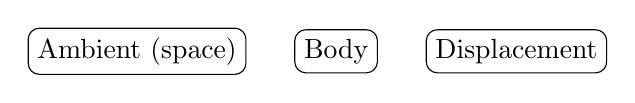
\begin{tikzpicture}[>=stealth,every node/.style={shape=rectangle,draw,rounded corners},node distance=0.05\linewidth,]
		    % create the nodes
			    \node[] (a1) {Ambient (space)}; %Physical space
			    \node[] (a2)[right =of a1] {Body}; %(Physical) system
			    \node[] (a3)[right =of a2] {Displacement}; %configuration
			\end{tikzpicture}
		\end{center}
	}
\end{frame}
\note[itemize]{
	\item In molte presentazioni di nozioni matematiche per concetto primitivo o nozione primitiva si intende un concetto che, per la propria semplicità ed intuitività, si rinuncia a definire mediante termini e concetti già definiti all'interno di un sistema formale, e che al contrario si sceglie di sfruttare per formulare la definizione di altri concetti; pertanto un concetto primitivo si accetta senza spiegazioni perché il suo significato è ovvio.
}
%-------------------------------------------------------------------------------------------------------------------------------------------------


%-------------------------------------------------------------------------------------------------------------------------------------------------
\begin{frame}[t]{Configuration Space: the Ambient}
	\begin{center}
		
\begin{tikzpicture}[>=stealth,every node/.style={shape=rectangle,draw,rounded corners},node distance=0.05\linewidth,]
	    % create the nodes
		    \node[red] (a1) {Ambient (space)}; %Physical space
		    \node[gray] (a2)[right =of a1] {Body}; %(Physical) system
		    \node[gray] (a3)[right =of a2] {Displacement}; %configuration
		\end{tikzpicture}	
	\end{center}
	\begin{columns}
		\begin{column}[T]{0.5\textwidth}
			\begin{itemize}
				\item The physical space, our universe.
				\item It is the stage on which the act of dynamics takes place.
			\end{itemize}
			\vspace{1em}
			\onslide<2->{					
				\begin{exblock}
					Consider a laboratory.
				\end{exblock}
			}
			\vspace{1em}
			\onslide<3->{
				\begin{mathblock}
					is the Euclidean space $E=\mathbb{R}^3$.
					\\				
					(fixed a \emph{Galilean observer}) 
				\end{mathblock}
			}		
		\end{column}
		\begin{column}[T]{0.5\textwidth}
			\onslide<2->{
				\begin{center}
					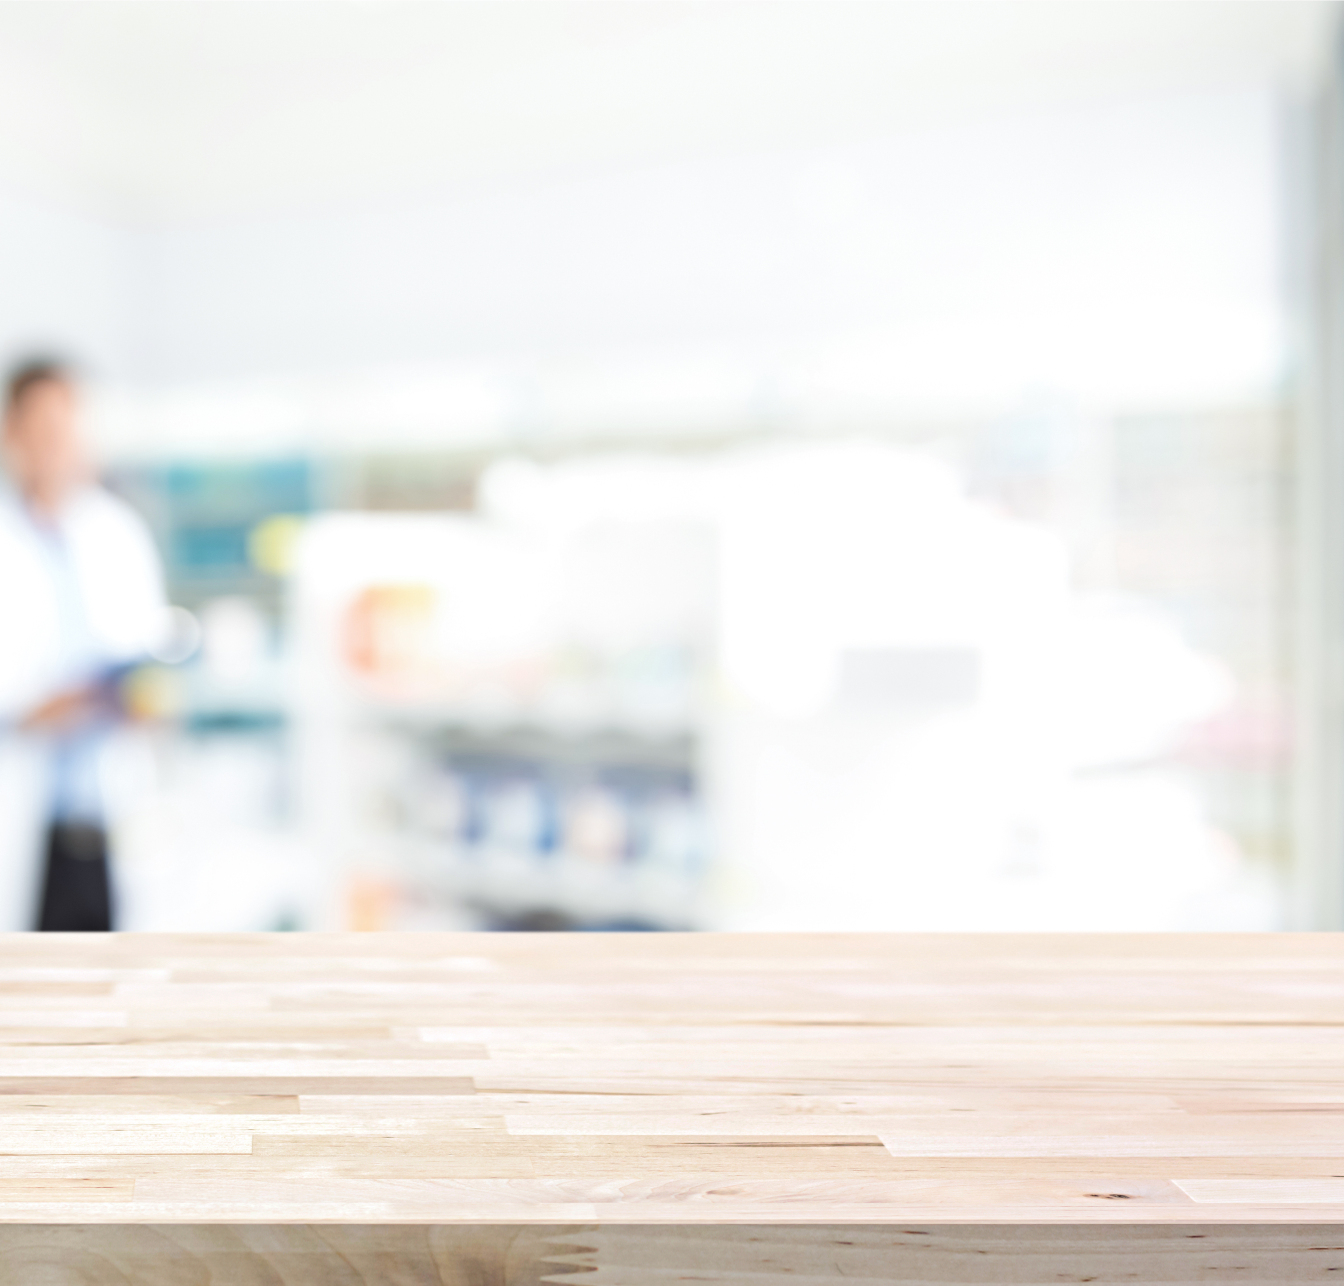
\includegraphics[width=\textwidth]{Pictures/emptylab}
				\end{center}
			}
		\end{column}
	\end{columns}
\end{frame}
\note[itemize]{
	\item
}
%-------------------------------------------------------------------------------------------------------------------------------------------------


%-------------------------------------------------------------------------------------------------------------------------------------------------
\begin{frame}[t]{Configuration Space: the Body}
	\begin{center}
		
\begin{tikzpicture}[>=stealth,every node/.style={shape=rectangle,draw,rounded corners},node distance=0.05\linewidth,]
	    % create the nodes
		    \node[gray] (a1) {Ambient (space)}; %Physical space
		    \node[red] (a2)[right =of a1] {Body}; %(Physical) system
		    \node[gray] (a3)[right =of a2] {Displacement}; %configuration
		\end{tikzpicture}
	\end{center}

	\begin{columns}
		\begin{column}[T]{0.5\textwidth}
			\begin{itemize}
				\item it is a bulk of matter, a portion of the ambient, we wish to study.
			\end{itemize}
								
			\vspace{1em}
			\only<2->{			
				\begin{exblock}
					Consider the bob of a rigid pendulum.
				\end{exblock}
			}

			\vspace{1em}
			\only<3->{
				\begin{mathblock}
					\begin{columns}
						\begin{column}{0.025\textwidth}
						\end{column}
						\begin{column}[T]{0.5\textwidth}
							is a submanifold $B\hookrightarrow E$ with boundary
							\vspace{-.5em}
							\begin{center}
								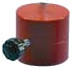
\includegraphics[width=.25\textwidth]{Pictures/bob}
							\end{center}
						\end{column}					
						\begin{column}[T]{0.45\textwidth}
							is a point in $B\in E$ (the center of mass).
							\begin{center}
								\tikz[] \node[scale=0.5,coordinate,fill=red,circle] (n1) {};	
							\end{center}						
						\end{column}							
					\end{columns}
					\begin{column}{0.025\textwidth}
					\end{column}
				\end{mathblock}
			}
			\vfill
%			\only<4->{
%				\begin{bracketbox}%{Key point:}
%					\small
%					Remind:
%					The ambient acts on the body via \emph{forces} and \emph{constraints}.
%				\end{bracketbox}
%			}	
		\end{column}
		\begin{column}[T]{0.5\textwidth}
				\begin{center}
					\includegraphics<1>[width=\textwidth]{Pictures/emptylab}
					\includegraphics<2->[width=\textwidth]{Pictures/Pendolab}					
				\end{center}
		\end{column}
	\end{columns}
\end{frame}
\note[itemize]{
	\item "è il protagonista della recita"
	\item remind the implied idea: 	The ambient acts on the body via \emph{forces} and \emph{constraints}.
}	
%-------------------------------------------------------------------------------------------------------------------------------------------------


%-------------------------------------------------------------------------------------------------------------------------------------------------
\begin{frame}[t]{Configuration Space: the displacement}
	\begin{center}
		
\begin{tikzpicture}[>=stealth,every node/.style={shape=rectangle,draw,rounded corners},node distance=0.05\linewidth,]
	    % create the nodes
		    \node[gray] (a1) {Ambient (space)}; %Physical space
		    \node[gray] (a2)[right =of a1] {Body}; %(Physical) system
		    \node[red] (a3)[right =of a2] {Displacement}; %configuration
		\end{tikzpicture}
	\end{center}

	\begin{columns}
		\begin{column}[T]{0.5\textwidth}
			\begin{itemize}
				\item is how the body is placed inside the space.
				\item configuration (spatial displacement) of the physical system admissible by the constraints.
			\end{itemize}
			\vspace{1em}
			\only<2->{
				\begin{exblock}[Pendulum]
					one of the possible positions where the bob can be placed allowed by the rod.		
				\end{exblock}
			}	
			\vspace{1em}
			\only<3->{
				\begin{mathblock}
					is a (smooth) function $B \to E$.				
				\end{mathblock}
			}					
			
		\end{column}
		\begin{column}[T]{0.5\textwidth}
			\begin{center}
				\includegraphics<1>[width=\textwidth]{Pictures/Pendolab}
				\only<2->{	
					\animategraphics[autoplay,palindrome,width=\textwidth]{5}{Pictures/pendolum-frame/pendo}{1}{9}
				}
			\end{center}
		\end{column}
	\end{columns}
\end{frame}
\note[itemize]{
	\item
}

%-------------------------------------------------------------------------------------------------------------------------------------------------

%-------------------------------------------------------------------------------------------------------------------------------------------------
\begin{frame}[t]{Configuration Space}
	%	
	\center
	\begin{zigzagbox}
		Neglect the fluff $\quad\rightsquigarrow\quad$ abstract (synthetic) mathematical setting
	\end{zigzagbox}
	
	\begin{columns}
		\begin{column}[T]{0.5\textwidth}
			\begin{itemize}
				\item<2-> Consider the set $Q$  of all the possible displacements (spatial configurations).
			\end{itemize}
			%			
			\vspace{1em}
			\onslide<3->{
				\begin{exblock}[Pendulum]
					$Q$ = 
						the locus of points on the plane with fixed distance from the pivot (the circle $S^1$).	
				\end{exblock}
			
			}			
			%			
			\vspace{1em}
			\onslide<4->{
				\alert{Upshot: $Q$ is a smooth manifold}
							
			\begin{defblock}[Configuration Space]
				Smooth manifold of all the system configurations admissible by the constraints.
			\end{defblock}			
			}
		\end{column}


		\begin{column}[T]{0.5\textwidth}
			\begin{center}
			\only<1>{				
				\resizebox{\textwidth}{!}{		
				    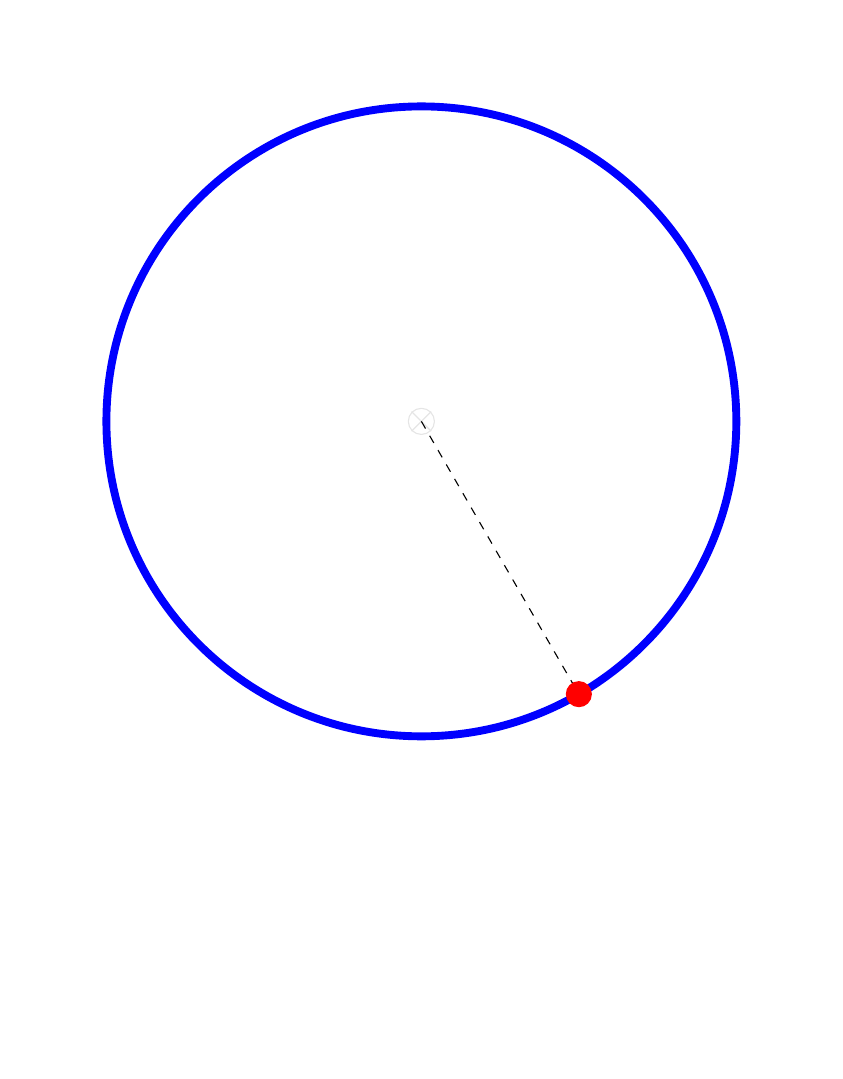
\begin{tikzpicture}
					    %frame
					    \draw[draw=none] (-5,-8) rectangle (5,5);
						% Support
						\coordinate (o) at (0,0);
						\node[cross out,draw,black!10] (0,0){};
						\node[circle,draw,black!10] (0,0){};
						% Bob's trajectory
						\draw[blue,line width=1mm,] (0,0) circle (4);
						% Rod + Bob
						\draw[dashed] (0,0) -- (-60:4) node[fill,circle,red](m){};
				    \end{tikzpicture}
				}
			}
			\only<2->{				
				\resizebox{\textwidth}{!}{		
					\pgfmathtruncatemacro\steps{50}
					\pgfmathtruncatemacro\maxtheta{30}
					\pgfmathtruncatemacro\pi{3.14}
					\begin{animateinline}[autoplay,loop]{10} % 5 fps, same as 0.2 s transduration
					  \multiframe{\steps}{i=0+1}{
					    \begin{tikzpicture}
					    \pgfmathsetmacro\fraction{\i/(\steps-1)}
						\pgfmathsetmacro\theta{\maxtheta*cos(360*\fraction)-90}
					    %frame
					    \draw[draw=none] (-5,-8) rectangle (5,5);
						% Support
						\coordinate (o) at (0,0);
						\node[cross out,draw,black!10] (0,0){};
						\node[circle,draw,black!10] (0,0){};
						% Bob's trajectory
						\draw[blue,line width=1mm] (0,0) circle (4);
						% Rod + Bob
						\draw[dashed] (0,0) -- (\theta:4) node[fill,circle,red](m){};
					    \end{tikzpicture}
					  }
					\end{animateinline}
				}
			}
			\end{center}
		\end{column}
	\end{columns}
\end{frame}
\note[itemize]{
	\item
}
%-------------------------------------------------------------------------------------------------------------------------------------------------

%-------------------------------------------------------------------------------------------------------------------------------------------------
\begin{frame}{Quick reminder: Smooth manifolds}
	\tcbset{colback=white,
	colbacktitle=white,
	colframe=red!70!black,
	boxrule=1pt,
	colupper=red!70!black,
	arc=15pt,
	}
		\begin{columns}[]
		\begin{column}{0.475\textwidth}
			\begin{tcolorbox}[enhanced,frame hidden,borderline={0.5pt}{0pt}{red!70!black}]
			Extrinsically:\\
			\color{black} 
			\emph{higher dimensional} surface 
			\\ smoothly embedded in $\mathbb{R}^N$.
			\\
			\small (for a suitably large $N$).		
			\end{tcolorbox}
	
			\center
			\onslide<2->{
				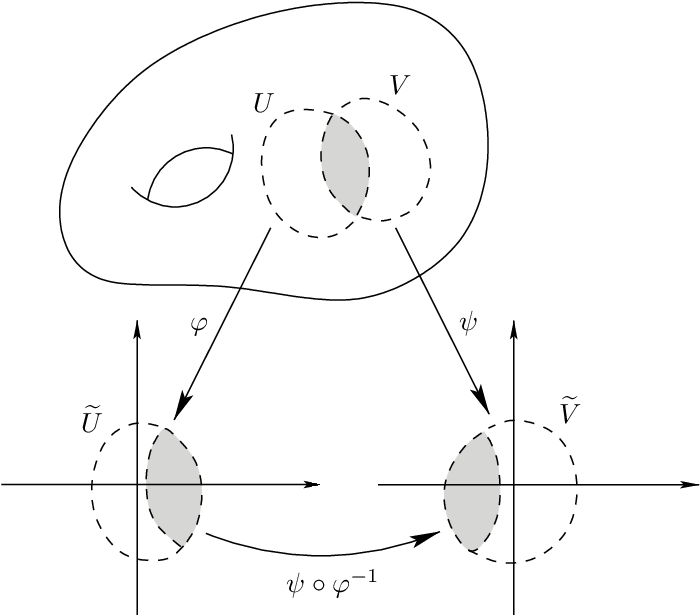
\includegraphics[width=.9\textwidth, height = 10em]{Pictures/smooth-mfd-Lee} 	
				%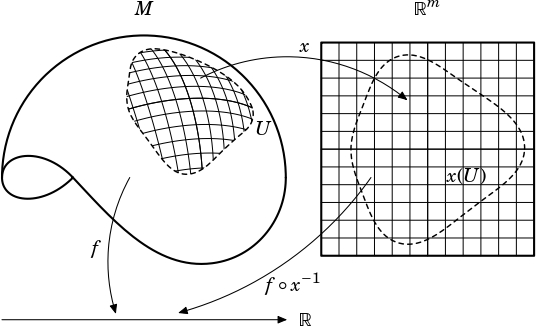
\includegraphics[width=.7\textwidth]{Pictures/LocalChart} 		
			}
		\end{column}
		\begin{column}{0.52\textwidth}
			\center
			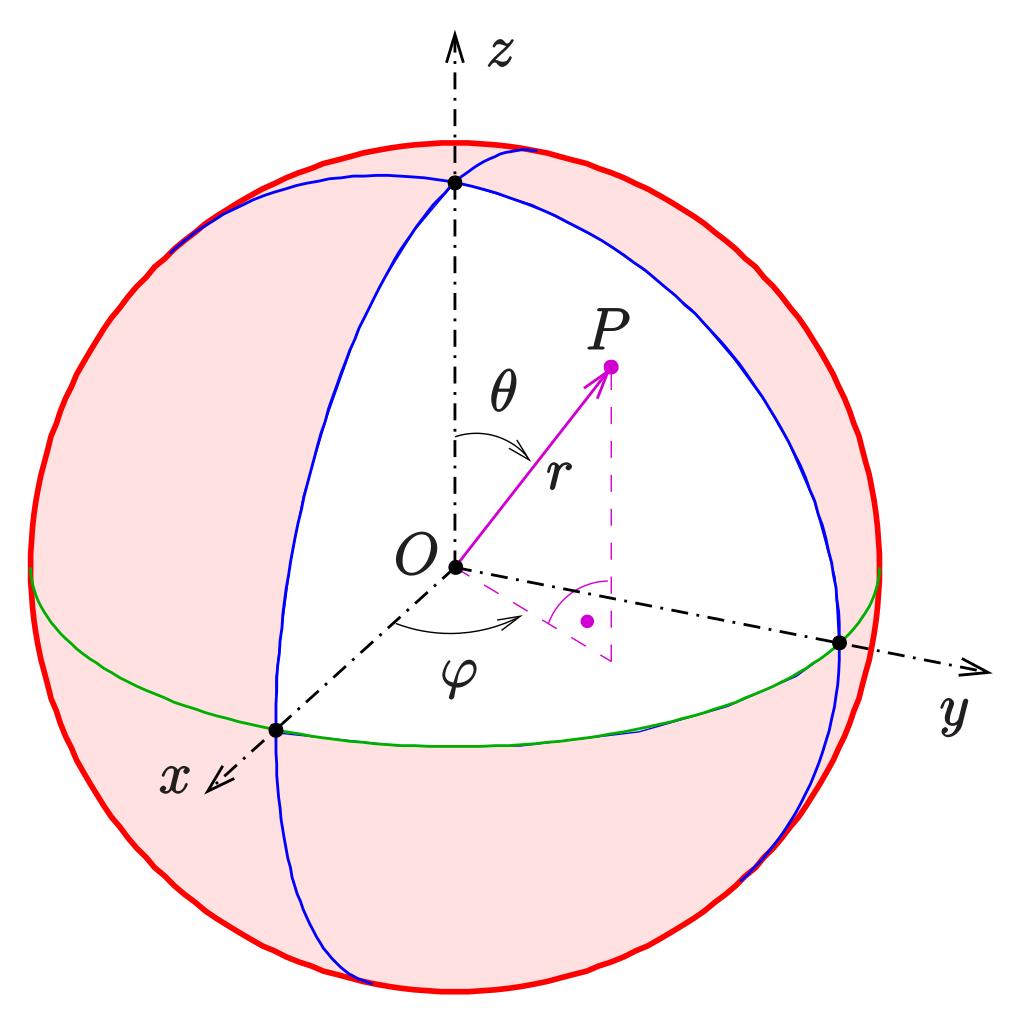
\includegraphics[width=.5\textwidth]{Pictures/embedded_sphere} 	
			
			\onslide<2->{
				\begin{tcolorbox}[enhanced,frame hidden,borderline={0.5pt}{0pt}{red!70!black}]
					Intrinsically:\\
					\color{black} 
					A topological spaces equipped with 
					\\ (a maximal atlas of compatible) 
					\\
					charts.
				\end{tcolorbox}			
			}			
		\end{column}
		\end{columns}
		
		\vfill
		\begin{columns}[]
			\begin{column}{0.1\textwidth}\end{column}
			\begin{column}{0.6\textwidth}
				\onslide<3->{
			\begin{tcolorbox}[enhanced,frame hidden,borderline={0.5pt}{0pt}{brown!70!black}]
				A reasonably general setting for defining:
				\begin{itemize}
					\item[•] Reference frames / coordinates (observers);
					\item[•] Smoothness.
				\end{itemize}
			\end{tcolorbox}
				}
			\end{column}
			\begin{column}{0.1\textwidth}\end{column}
		\end{columns}






\end{frame}
\note[itemize]{
	\item
}
%-------------------------------------------------------------------------------------------------------------------------------------------------


%-------------------------------------------------------------------------------------------------------------------------------------------------
\begin{frame}[t]{Configuration Space: a slightly more difficult example}
		\center
	\begin{bracketbox}
		Double pendulum.
	\end{bracketbox}
	

	\vfill
	\only<1-3>{
		\begin{columns}[T]
			\begin{column}{0.5\textwidth}
				\begin{center}
					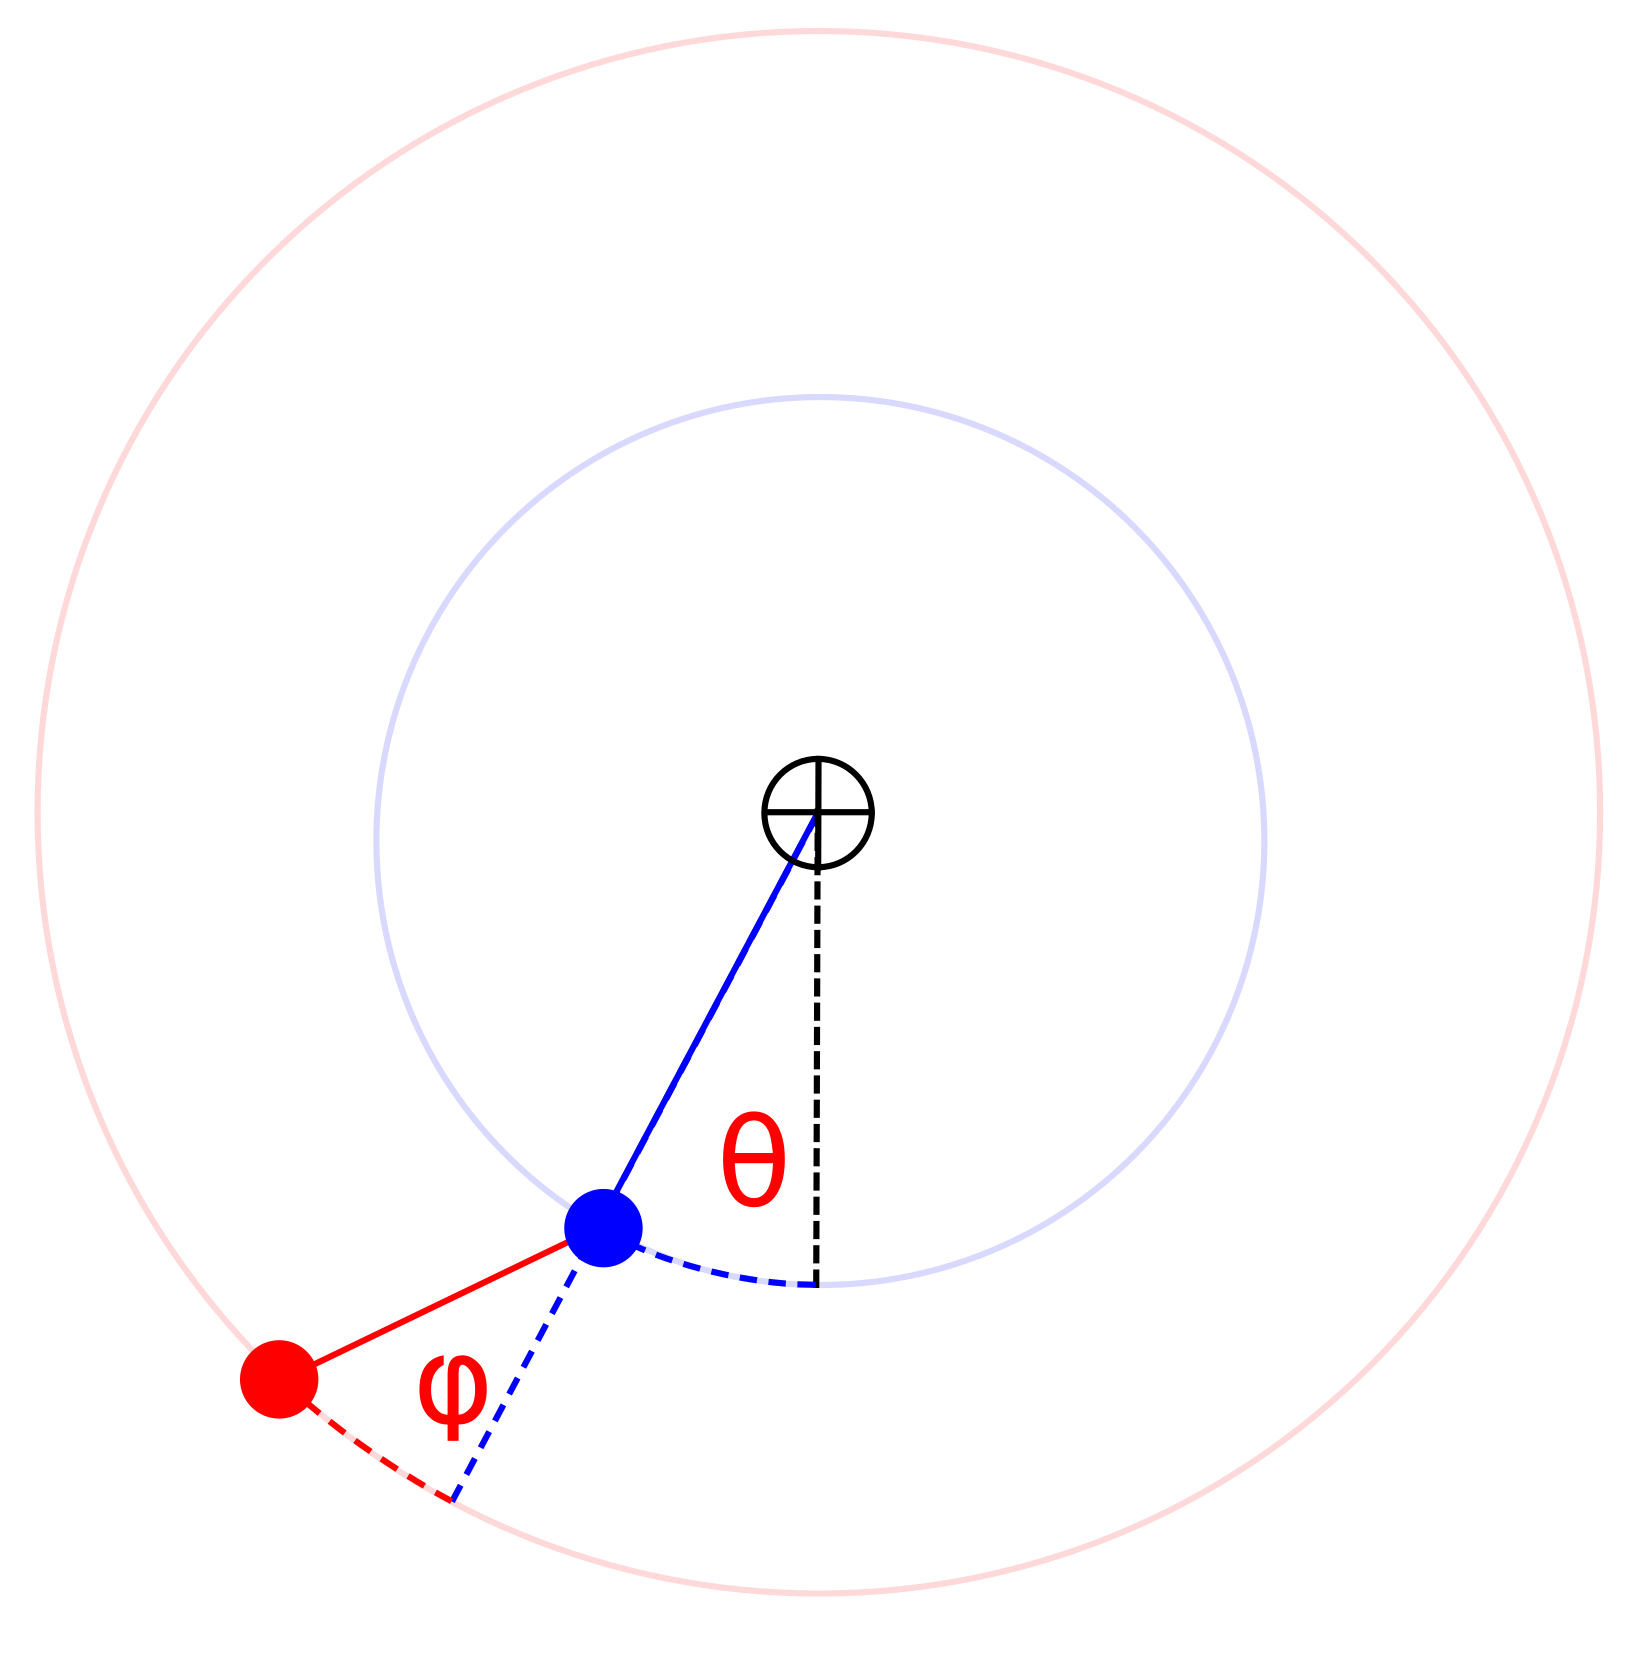
\includegraphics[width=.75\textwidth]{Pictures/bipend-abstract}	
				\end{center}
			\end{column}
			\begin{column}{0.5\textwidth}
				\begin{center}
					\only<1>{
						\noindent Toy model for:
						\begin{center}
							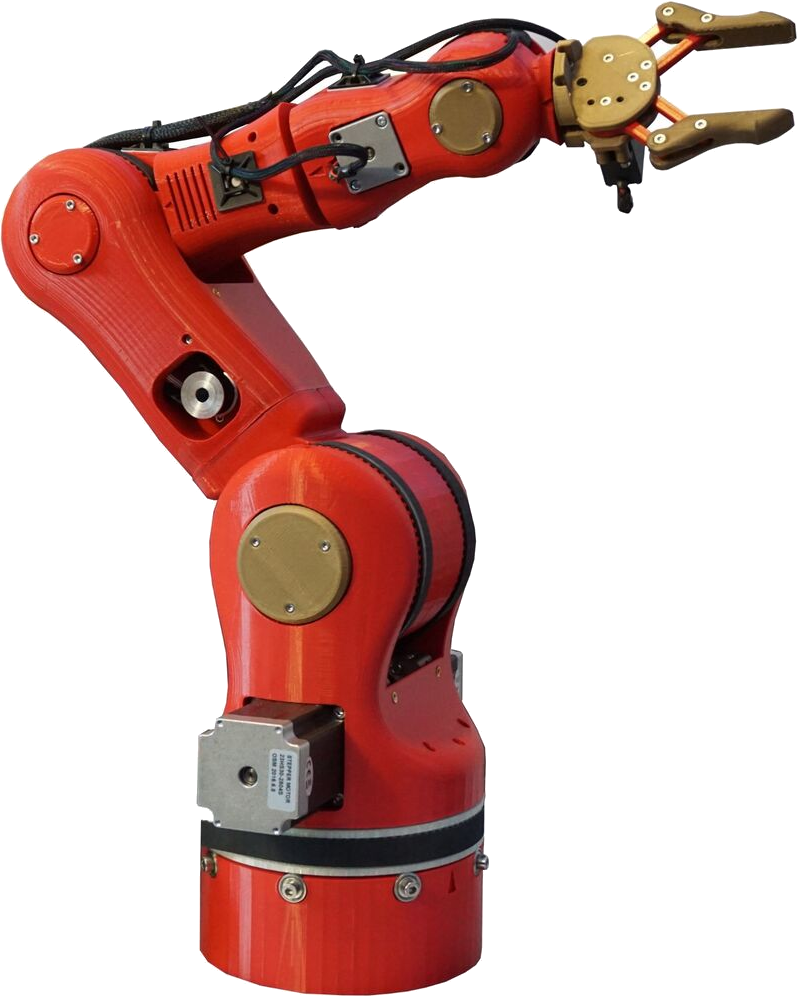
\includegraphics[width=.55\textwidth]{Pictures/robo_arm}
						\end{center}
						mechanical arms.
					}
					\only<2>{
						\noindent Toy model for:
						\begin{center}
							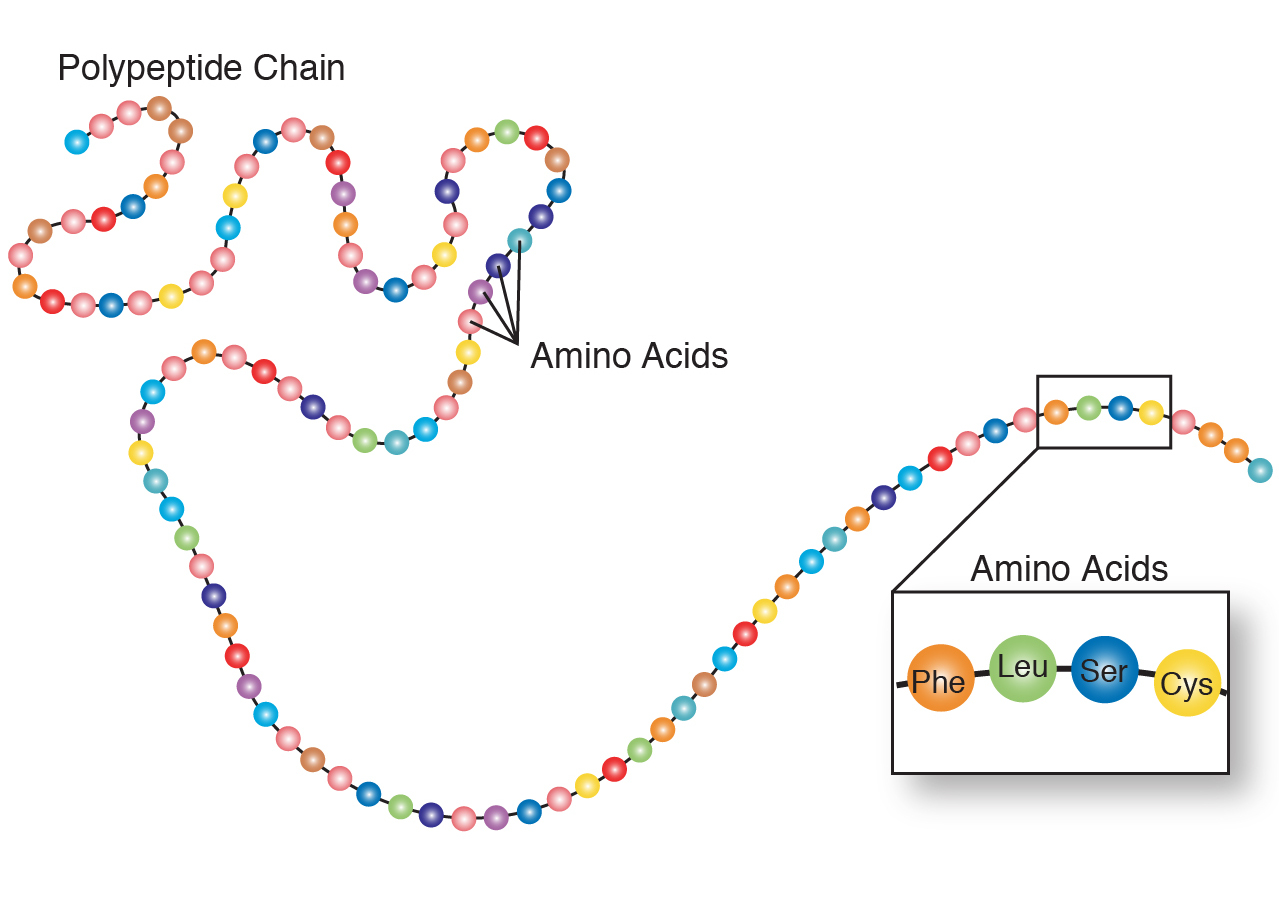
\includegraphics[width=.65\textwidth]{Pictures/amino_acids}
						\end{center}
						Proteins (amino acid chains).	
					
					}
					\only<3>{
						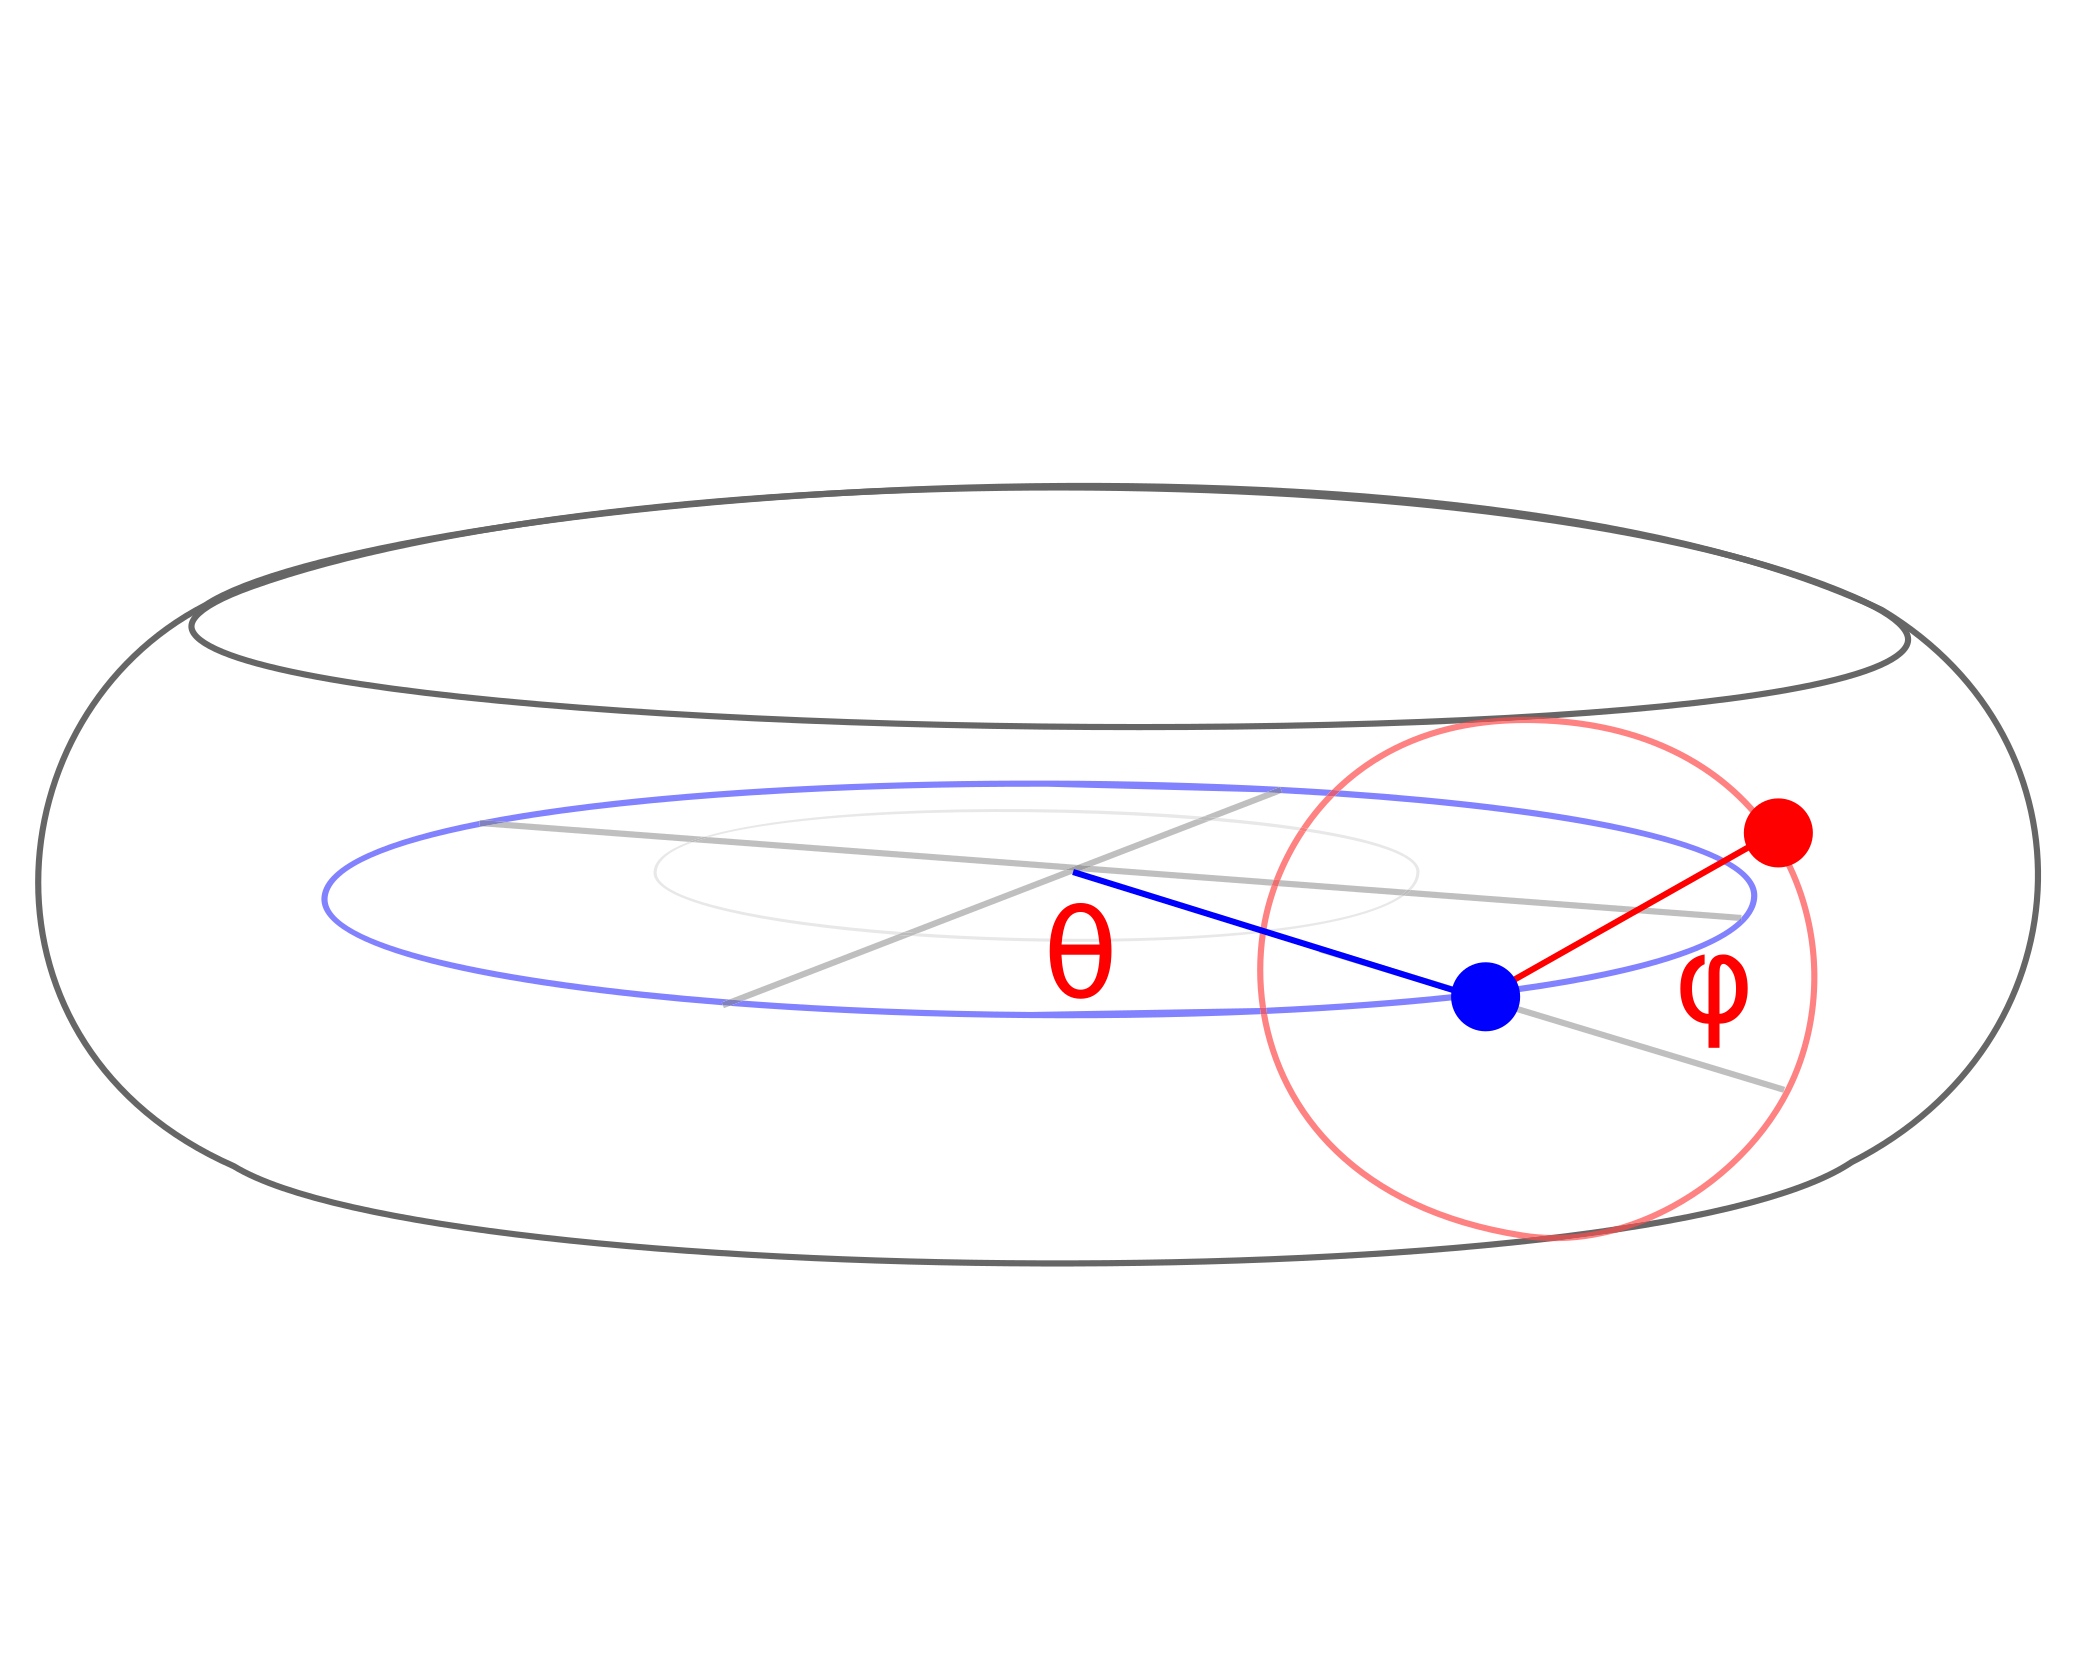
\includegraphics[width=.75\textwidth]{Pictures/bipend-phase}	
					}
				\end{center}
			\end{column}
		\end{columns}	
	}
	\only<4->{
		\animategraphics[autoplay,palindrome,width=\textwidth]{5}{Pictures/lessig-pibend-frame/bipend-}{2}{6}
	}
	\vfill
	\onslide<3->{\center\alert{Configuration space is a Torus}}


\end{frame}
\note[itemize]{
	\item per quanto sia un toy model è il primo passo per modellizzare una proteina. (Catena di amminoacidi posti a distanza pressochè costante fra di loro)
	\item This case (bi-pendulum) examplify how constraints can be enforced intrinsically choosing an appropriate geometric framework. (2-coordinates instead of the 4 x-y coordinates needed to fix the two endopoints.

}
%-------------------------------------------------------------------------------------------------------------------------------------------------

\end{document}

%-------------------------------------------------------------------------------------------------------------------------------------------------
\subsection{Space of States}
%-------------------------------------------------------------------------------------------------------------------------------------------------
	%- HandOut Flag -----------------------------------------------------------------------------------------
\newif\ifHandout

%- D0cum3nt ----------------------------------------------------------------------------------------------
\documentclass[beamer,10pt]{standalone}   
%\documentclass[beamer,10pt,handout]{standalone}  \Handouttrue  

%- HandOut Flag -----------------------------------------------------------------------------------------
\ifHandout
	\setbeameroption{show notes} %print notes   
\fi

	
%- Packages ----------------------------------------------------------------------------------------------
\usepackage{custom-style}
\usetikzlibrary{positioning}
\usepackage{multicol}


%--Beamer Style-----------------------------------------------------------------------------------------------
\usetheme{toninus}
\usepackage{animate}
\usetikzlibrary{positioning, arrows}
\usetikzlibrary{shapes}
\usepackage{ifthen}

\begin{document}
%-------------------------------------------------------------------------------------------------------------------------------------------------
\begin{frame}{From \emph{configurations} to \emph{states}}
\begin{columns}[T]
	\begin{column}{0.5\textwidth}
		\begin{center}
			\resizebox{\textwidth}{!}{		
				\pgfmathtruncatemacro\steps{50}
				\pgfmathtruncatemacro\maxtheta{30}
				\pgfmathtruncatemacro\pi{3.14}
				\begin{animateinline}[autoplay,loop]{10} % 5 fps, same as 0.2 s transduration
				  \multiframe{\steps}{i=0+1}{
				    \begin{tikzpicture}
				    \pgfmathsetmacro\fraction{\i/(\steps-1)}
					\pgfmathsetmacro\theta{\maxtheta*cos(360*\fraction)-90}
					\pgfmathsetmacro\v{-1*sin(360*\fraction)}
				
				    %frame
				    \draw[draw=none] (-6,-8) rectangle (6,6);		
					% Support
					\coordinate (o) at (0,0);
					\node[cross out,draw,black!10] (0,0){};
					\node[circle,draw,black!10] (0,0){};
					% Bob's trajectory
					\draw[blue,line width=1mm] (0,0) circle (4);
					% Rod + Bob
					\draw[dashed] (0,0) -- (\theta:4) node[fill,circle,red](m){};

					% Velocity
					\ifthenelse{\equal{\i}{0}}
           			{}
           			{\draw[-latex,green!80!black,line width=1mm] (m) -- node[green!80!black,below right]{$\vec{v}$}($(m)!\v!-90:(o)$);}
				    \end{tikzpicture}
				  }
				\end{animateinline}
			}
		\end{center}
	\end{column}
	\begin{column}{0.5\textwidth}
		\begin{itemize}
			\item Knowing the position is not sufficient to determine the evolution of the system.
			\item (Displacement encode statics, one must know how configurations evolves in time)
			\item One needs to know also the velocity (or better, the momentum).
		\end{itemize}

		\vspace{1em}
		\onslide<2->{
			\begin{upshotblocksimp}
				Upshot:
				Configurations $\neq$ \emph{States}
			\end{upshotblocksimp}			
		}
	\end{column}
\end{columns}
\end{frame}
\note[itemize]{
	\item
}
%-------------------------------------------------------------------------------------------------------------------------------------------------

%-------------------------------------------------------------------------------------------------------------------------------------------------
\begin{frame}{Quick reminder: Trajectories, velocities, Tangent spaces}



	\begin{columns}
			\begin{column}{.6\linewidth}
				\only<1>{\includegraphics[width=\textwidth]{Pictures/Vector1} }
				\only<2>{\includegraphics[width=\textwidth]{Pictures/Vector2} }
				\only<3->{\includegraphics[width=\textwidth]{Pictures/Vector3} }
			\end{column}
			\begin{column}{.4\linewidth}
				\begin{itemize}
					\item Well defined notion of smooth curves $C^\infty(\mathbb{R},M)$ on smooth manifolds.
					\item<2-> Velocity of curves can be computed through charts.
				\end{itemize}
			\end{column}				
	\end{columns}
		\vfill
		\begin{itemize}
			\item<3-> Comparing velocities in local chars yields an equivalence relations of curves passing through a point $p \in M$
		\end{itemize}
		
		\vfill
		\onslide<4->{
		\begin{defblock}[Tangent space at $p\in M$]
			\begin{displaymath}
				T_p M \coloneqq
   				\left\{
				\parbox{.55\linewidth}{Vector space of equivalence classes of curves \\with equal local velocity at $p\in M$.}
				 \right\}.
			\end{displaymath}
		\end{defblock}
		}
\end{frame}
\note[itemize]{
	\item
}
%-------------------------------------------------------------------------------------------------------------------------------------------------

%-------------------------------------------------------------------------------------------------------------------------------------------------
\begin{frame}{Phase Space (I)}
\begin{columns}[T]
	\begin{column}{0.5\textwidth}
		\begin{center}
			\resizebox{\textwidth}{!}{
				\begin{tikzpicture}
					\node[draw=none] (o) at (0, 0) {o};
				    %frame
				    \draw[draw=none] (-6,-8) rectangle (6,6);				
					\draw[draw=none](0,0)--(-90:4)node[circle, fill, minimum size=5pt,
				              inner sep=0pt, outer sep=0pt](p){};
					\draw[green,line width=1mm] ($ (p)!3.5cm!90:(o) $) -- ($ (p)!3.5cm!270:(o) $);
					\draw[green,dashed,line width=1mm] ($ (p)!4.5cm!90:(o) $) -- ($ (p)!4.5cm!270:(o) $);
					\draw[blue,line width=1mm] (0,0) circle (4);
				\end{tikzpicture}
			}
			%
		\end{center}
	\end{column}
	\begin{column}{0.5\textwidth}
 		\begin{itemize}
 			\item consider {\bf a} configuration.
 			\item all possible velocities are encoded by points on the tangent line at the given configuration \\(\emph{Tangent space}).
 		\end{itemize}
	\end{column}
\end{columns}
\end{frame}
\note[itemize]{
	\item
}
%-------------------------------------------------------------------------------------------------------------------------------------------------



%-------------------------------------------------------------------------------------------------------------------------------------------------
\begin{frame}{Phase Space (II)}
\begin{columns}[T]
	\begin{column}{0.5\textwidth}
		\begin{center}
			\only<1>{
			\resizebox{\textwidth}{!}{
				\begin{tikzpicture}
					\node[draw=none] (o) at (0, 0) {o};
				    %frame
				    \draw[draw=none] (-6,-8) rectangle (6,6);						
					\foreach \x in {0,30,...,360}{
						\draw[draw=none](0,0)--(\x:4)node[circle, fill, minimum size=5pt,
					              inner sep=0pt, outer sep=0pt](p){};
					\draw[green,line width=1mm] ($ (p)!3.5cm!90:(o) $) -- ($ (p)!3.5cm!270:(o) $);
					\draw[green,dashed,line width=1mm] ($ (p)!4.5cm!90:(o) $) -- ($ (p)!4.5cm!270:(o) $);
					}
						\draw[blue,line width=1mm] (0,0) circle (4);
				\end{tikzpicture}
			}}
			%
			\only<2->{
			\resizebox{.7\textwidth}{!}{
				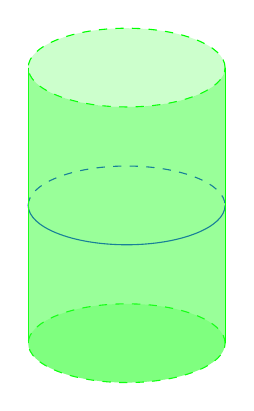
\begin{tikzpicture}
					\draw[green,dashed,fill=green!20] (0,0) ellipse (1.25 and 0.5);
					\draw [blue](-1.25,-1.75) arc (180:360:1.25 and 0.5);
					%\draw [blue,dashed] (-1.25,-3.5) arc (180:360:1.25 and -0.5);
					\draw[green,dashed,fill=green!20] (0,-3.5) ellipse (1.25 and 0.5);
					\draw [blue,dashed] (-1.25,-1.75) arc (180:360:1.25 and -0.5);
					\draw [green](-1.25,0) -- (-1.25,-3.5);
					\draw [green](1.25,-3.5) -- (1.25,0);  
					\fill [green!80,opacity=0.5] (-1.25,0) -- (-1.25,-3.5) arc (180:360:1.25 and 0.5) -- (1.25,0) arc (0:180:1.25 and -0.5);
				\end{tikzpicture}		
%				\begin{tikzpicture}
%				  \node[cylinder,draw=black,thick,aspect=0.7,minimum height=4cm,minimum width=2.5cm,shape border rotate=90,cylinder uses custom fill, cylinder body fill=green!30,cylinder end fill=green!10] (A) {\phantom{A}};
%				  \draw[dashed]
%				    let \p1 = ($ (A.after bottom) - (A.before bottom) $),
%				        \n1 = {0.5*veclen(\x1,\y1)-\pgflinewidth},
%				        \p2 = ($ (A.bottom) - (A.after bottom)!.5!(A.before bottom) $),
%				        \n2 = {veclen(\x2,\y2)-\pgflinewidth}
%				  in
%				    ([xshift=-\pgflinewidth] A.before bottom) arc [start angle=0, end angle=180,
%				    x radius=\n1, y radius=\n2];
%				\end{tikzpicture}	
}
			}
		\end{center}
	\end{column}
	\begin{column}{0.5\textwidth}
		\vspace{1.5em}
 		\begin{itemize}
 			\item Consider {\bf all possible} configurations.
 			\item Collect all possible pairs of position/momentum.
 			%\item points on the \emph{Tangent space}
 		\end{itemize}
		\vspace{1.5em} 		
 		\begin{itemize}
 			\item<2-> joining together all "tangent" space in a smooth and non-overlapping manner...
 		\end{itemize}
		\onslide<3->{
			\begin{upshotblocksimp}
				Upshot:
				\color{black}
					Collectively, all the possible tangent vector constitute another manifold called the \emph{Tangent Bundle}
					\begin{displaymath}
						TQ = \coprod_{q \in Q} T_q Q
						~.
					\end{displaymath}
				(\emph{Space of generalized velocities})		
			\end{upshotblocksimp}					
		} 		
	\end{column}
\end{columns}
\end{frame}
\note[itemize]{
	\item  		
 		Collect all possible pair of position and momentum
 		
 		Informally, the tangent bundle of a manifold (which in this case is a circle) is obtained by considering all the tangent spaces (top), and joining them together in a smooth and non-overlapping manner (bottom).

}
%-------------------------------------------------------------------------------------------------------------------------------------------------

%-------------------------------------------------------------------------------------------------------------------------------------------------
\begin{frame}{Phase Space}
\begin{columns}[T]
	\begin{column}{0.5\textwidth}
		\begin{center}
			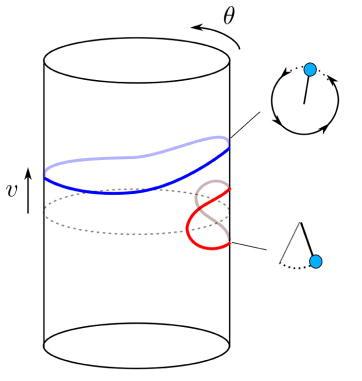
\includegraphics[width=\textwidth]{Pictures/pendo-phasespace}
		\end{center}
	\end{column}
	\begin{column}{0.5\textwidth}
 		\begin{itemize}
 			\item Consider {\bf all possible} configurations.
 			\item Collect all possible pairs of position/momentum.
 		\end{itemize}
		
		\vspace{1em}		
		\begin{defblock}[Phase Space]
			\begin{itemize}
				\item[=] collection of all \emph{states}
				\item[=] set of every possible "initial datas" (sufficient to reconstruct the motion).
			\end{itemize}
		\end{defblock}

		\vspace{1em}				
		\begin{mathblock}
			The Phase space is a \underline{symplectic} smooth manifold $(M)$.
		\end{mathblock}		
		
	\end{column}
\end{columns}
\end{frame}
\note[itemize]{
	\item You get an infinite cylinder (in the case of bipendulum I cannot picture it because we go directly into more than 2 dimensions.
	\item ho disegnato due traiettori sul fase space per mostrare come due natural motions si possono rappresentare bene qui sopra.
	\item per capire il significato di dell'aggettivo simplettico dobbiamo introdurre qualche altro interprete.

}
%-------------------------------------------------------------------------------------------------------------------------------------------------

%-------------------------------------------------------------------------------------------------------------------------------------------------
\begin{frame}{A little clarification on velocities vs momenta}
	\begin{itemize}
		\item In most cases: fixing configuration and velocity fix the state of the system.
		\item However, we consider the dual bundle $T^\ast Q$ as the phase space of the system.
	\end{itemize}
	\pause
	\vfill
	Reasoning: (understand elements in $T^\ast_q Q$ as \emph{mechanical momenta})
	\begin{itemize}
		\item $v\in T_q Q$ measures the rate of change of the displacement $q$ of the system.
		\item $p \in T^\ast_q Q$ measures the rate of change of the kinetic energy of the system w.r.t. a certain variation $\delta v$ of the velocity
		\vspace{-.5em}
		  \begin{alignat*}{2}
			  p: T_q Q &\longrightarrow& \mathbb{R} \\
		  	\delta v &\longmapsto& \delta T
		  \end{alignat*}		
	\end{itemize}

	\pause
	\begin{exblock}[Point-particle in $2D$ space \qquad {\small ( $Q=\mathbb{R}^2$)}]
		\begin{columns}[T]
			\begin{column}{.25\linewidth}
				\resizebox{\textwidth}{!}{
					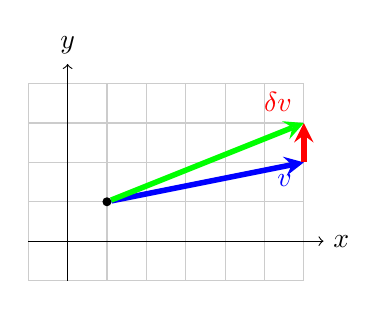
\begin{tikzpicture}
					  \draw[step=.5,thin,gray!40] (-.5,-.5) grid (3,2);
					  \draw[->] (-.5,0)--(3.25,0) node[right]{$x$};
					  \draw[->] (0,-.5)--(0,2.25) node[above]{$y$};
					  \node[draw,circle,fill,inner sep=1pt,] at (.5,.5) (q) {};
					  \draw[line width=2pt,blue,-stealth](q)--(3,1) node[anchor=north east]{$\boldsymbol{v}$};
					  \draw[line width=2pt,red,-stealth](3,1)--(3,1.5) node[anchor=south east]{$\boldsymbol{\delta v}$};
					  \draw[line width=2pt,green,-stealth](q)--(3,1.5) node[anchor=south west]{};
					\end{tikzpicture}
				}			
			\end{column}
			\begin{column}{.80\linewidth}
				Recall from bachelor courses: \quad $
					T = \dfrac{1}{2} m \boldsymbol{v}\cdot \boldsymbol{v} $
				
				Add a perturbation $\boldsymbol \delta v$ to the velocity $\boldsymbol v $.
				{\tiny (Neglecting II-order variations)} :
				\vspace{-.5em}				
				$$ \delta T = m~ \boldsymbol{v}\cdot \boldsymbol{\delta v} = p ( \boldsymbol{\delta v})$$
			\end{column}		
		\end{columns}
	\end{exblock}
	\vfill
	\pause
		\begin{upshotblocksimp}
			Motivation (a posteriori): 
			\color{blue}
			$T^\ast Q$ is naturally symplectic.
		\end{upshotblocksimp}	

\end{frame}
\note[itemize]{
	\item In most cases: fixing configuration adn velocity fix the state of the system.It is customary to consider the dual bundle $T^\ast Q$ as the phase space of the system.
	\item Although fixing a point in $TQ$ fixes the state of the system. In the context of geo. mech. is customary to  understand $T^\ast Q$ as the phase space of the system.
	\item idea: elements of $T_q Q$ measure the rate of change in the displacement of the system, elements of $T_q^\ast Q$ measure the change in kinetic energy of the system (encompassing somewhat the energy encoded by the motion and the system inertia).
	\item Formally, generalized momenta are $P: T_q Q \to \mathbb{R}$ such that, given a state of configuration $q$ and momenta $p$, for any variation $\delta \vec{v}\in T_q Q$, $P(\delta \vec{v})$ measure the variation $\delta T$ in the kinetic energy of the system.
	\item Per completezza: questa caratterizzazione del momento meccanico ha origine dal formalismo Lagrangiano.	
	
	\item What about the definition of linear momentum $\boldsymbol{p} = m \boldsymbol{v}$ learnt in high-school?
				\\
				It's still good since $p = m \boldsymbol{p} \cdot - $ but a little misleading because  based on the existence of an inner product on $Q=\mathbb{R}^3$ which does not exists in general.	
	\item a more precise justification for the fact that "momenta are covector" follows from  the Lagrangian formalism\url{https://math.stackexchange.com/questions/1235015/momentum-a-cotangent-vector}.
}
%-------------------------------------------------------------------------------------------------------------------------------------------------



\end{document}


%-------------------------------------------------------------------------------------------------------------------------------------------------
\section{Observables and time evolution}
\checkpoint	
%-------------------------------------------------------------------------------------------------------------------------------------------------
\subsection{Measurable quantities}
\subsection{Hamiltonian evolutions}
	%+----------------------------------------------------------------------------+
%| SLIDES: 
%| Chapter: Observables - Hamiltonians - Symplectic structure
%| Author: Antonio miti
%| Event: Phd Colloquium - What is ... Geometric mechanics?
%+----------------------------------------------------------------------------+

%- HandOut Flag -----------------------------------------------------------------------------------------
\makeatletter
\@ifundefined{ifHandout}{%
  \expandafter\newif\csname ifHandout\endcsname
}{}
\makeatother

%- D0cum3nt ----------------------------------------------------------------------------------------------
\documentclass[beamer,10pt]{standalone}   
%\documentclass[beamer,10pt,handout]{standalone}  \Handouttrue  

\ifHandout
	\setbeameroption{show notes} %print notes   
\fi

	
%- Packages ----------------------------------------------------------------------------------------------
\usepackage{custom-style}
\usetikzlibrary{positioning}
\usepackage{multicol}
\usepackage[thinlines]{easytable}

%--Beamer Style-----------------------------------------------------------------------------------------------
\usetheme{toninus}
\usepackage{animate}
\usetikzlibrary{positioning, arrows}
\usetikzlibrary{shapes,shapes.callouts}

\begin{document}

%-------------------------------------------------------------------------------------------------------------------------------------------------
\begin{frame}{Observables}
	An observables is:
	\vfill
	\begin{columns}[T]
		\begin{column}{0.5\textwidth}
			\begin{itemize}
				\item a procedure to read a certain quantity (a number) out of any state of the system
				\item<2-> a quantity that can be measured with a device. 
			\end{itemize}				
			%
			\vspace{.5em}
			\onslide<3->{
				\begin{exblock}[Pendulum inclination]
					Measure the inclination of the rod with a goniometer.
				\end{exblock}			
			}
			%
			\vspace{.5em}
			\onslide<4->{
				\begin{mathblock}
					Observables are given by smooth functions on the phase space $M$:
					\begin{displaymath}
						\mathcal{O}=C^{\infty}(M)~.
					\end{displaymath}
				\end{mathblock}
			}
		\end{column}
		\begin{column}{0.5\textwidth}
			\begin{center}
				\ifHandout 
					\includegraphics<3>[width=.7\textwidth]{Pictures/observo}				
				\else
					\includegraphics<1>[width=.9\textwidth]{Pictures/pendo60-nogonio}
					\includegraphics<2>[width=.9\textwidth]{Pictures/pendo60}
					\includegraphics<3>[width=.9\textwidth]{Pictures/observo}
				\fi
				
				\only<3>{
					\tikz[overlay,remember picture]
					{
						\node[ellipse callout,fill=white!50,
			               draw=black,
			               anchor=base]            
			            	 (base) at ($(current page.east)+(-5,3)$) [rotate=-0,text width=1.5cm,align=center,callout relative pointer={(-.3,-.8)}] 
			            	 {Measure: \\$\theta=\pi/3$\\$\phantom{\theta}\cong 1.05$};
					}	
				}
				\only<4>{
					\resizebox{.9\textwidth}{!}{				
						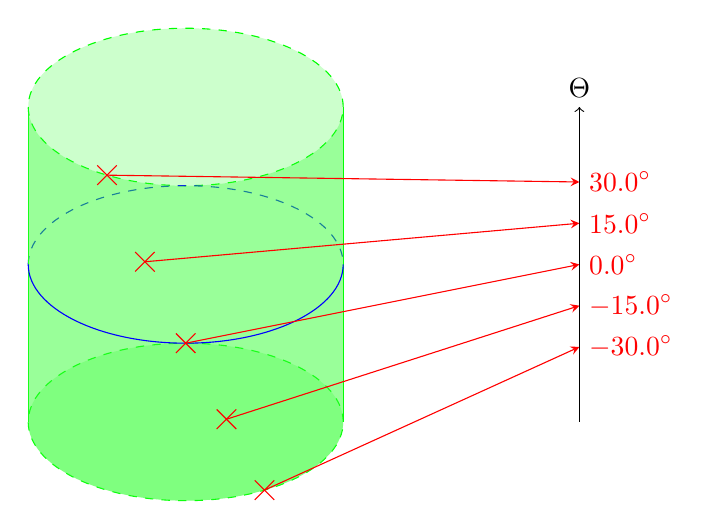
\begin{tikzpicture}
							\pgfmathtruncatemacro\steps{4}
							\pgfmathtruncatemacro\mintheta{-120}
							\pgfmathtruncatemacro\maxtheta{-60}
							\pgfmathsetmacro\deltatheta{(\maxtheta-\mintheta)/(\steps)}
							\pgfmathsetmacro\viewpitch{30}
							\pgfmathsetmacro\diam{2}
							\pgfmathsetmacro\H{4}
							\pgfmathsetmacro\deltaH{(\H)/(\steps)}
							\pgfmathsetmacro\X{\diam}
							\pgfmathsetmacro\Y{\diam*sin(\viewpitch)}	
							\pgfmathsetmacro\vel{\diam/4}	
		
							\draw[green,dashed,fill=green!20] (0,0) ellipse ({\X} and {\Y});
							%\draw [blue,dashed] (-1.25,-3.5) arc (180:360:1.25 and -0.5);
							\draw[green,dashed,fill=green!20] (0,-{\H}) ellipse ({\X} and {\Y});
							\draw [blue,dashed] (-{\X},-{.5*\H}) arc (180:360:{\X} and -{\Y});
							\draw [green](-{\X},0) -- (-{\X},-{\H});
							\draw [green]({\X},-{\H}) -- ({\X},0);  
							\fill [green!80,opacity=0.5] (-{\X},0) -- (-{\X},-{\H}) arc (180:360:{\X} and {\Y}) -- ({\X},0) arc (0:180:{\X} and -{\Y});
							\draw [blue](-\X,-{.5*\H}) arc (180:360:{\X} and {\Y});

							\foreach \i in {0,1,...,\steps}{
								\pgfmathsetmacro\h{-\i*\deltaH}
								\pgfmathsetmacro\theta{\mintheta + \i*\deltatheta}	
								\pgfmathsetmacro\thetalabel{-\theta -90}	
									
								\draw[red,-stealth] (0,\h)++({cos(\theta)*\X},{sin(\theta)*\Y}) node[draw,cross out]{}  -- (5,{pi*2*(\thetalabel)/180-\H/2})node[right] {${\thetalabel}^\circ$};
							}
							\draw[->] (5,-{\H})--(5,0) node[above] {${\Theta}$}; % ordinate
						\end{tikzpicture}	
					}
				}
			\end{center}
		\end{column}
	\end{columns}
\end{frame}
\note[itemize]{
	\item Observation /Measure, procedure to extract a number from a physical system.	E.g. a measure with a device	

}
%-------------------------------------------------------------------------------------------------------------------------------------------------

%-------------------------------------------------------------------------------------------------------------------------------------------------
\begin{frame}[t]{Hamiltonian: Energy observable}
	A certain observable takes a central role:
	\vfill
	\begin{columns}[T]
		\begin{column}{0.5\textwidth}
			\begin{defblock}[Hamiltonian observable]
				Observable measuring the total energy of the system.
				\begin{displaymath}
					H = \text{Kinetic} + \text{Potential}
				\end{displaymath}
			\end{defblock}		
			\vspace{1em}
			\onslide<2->{
				\begin{exblock}[Pendulum]
					In practical terms: $H$ is a device measuring the battery charge dissipated by a motor to lift the bob to a certain height.	
				\end{exblock}
			}			
			%
		\end{column}
		\begin{column}{0.5\textwidth}
			\begin{center}
				\onslide<2->{	
					\animategraphics[autoplay,palindrome,width=\textwidth]{1}{Pictures/pendolabenergy-}{0}{1}
				}			
			\end{center}
		\end{column}
	\end{columns}
	\vfill
	\onslide<3->{
		\begin{upshotblocksimp}
			Upshot: $H$	embodies how the ambient acts on the system and the system's inertia to respond to the external forces.
		\end{upshotblocksimp}		
	}


\end{frame}
\note[itemize]{
	\item among all possible observables "Energy" has a pivotal role:
	\item Without being too philosophica. Consider our pendulum system.
	\item \emph{potential energy} account the interaction of the "ambient" with the "body".
	\item \emph{kinetic energy} is the energy of the motion.
}
%-------------------------------------------------------------------------------------------------------------------------------------------------

%-------------------------------------------------------------------------------------------------------------------------------------------------
\begin{frame}{Symplectic structure - an intuition -}
	\center
	\alert{Phase spaces has a canonical \underline{symplectic structure}}
	\vfill
	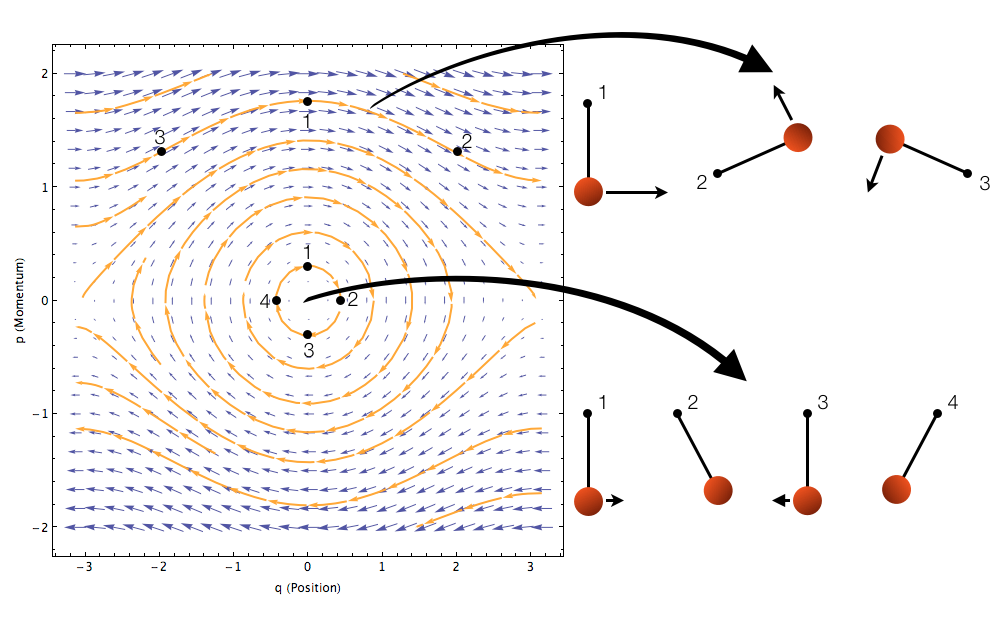
\includegraphics[width=.85\textwidth]{Pictures/pendo-hamiltonianfield}	
	\vfill
	\begin{itemize}
		\item Is  a prescription of an \emph{Hamiltonian field} $v_f$ to any observable $f$.
		\item The flow gives the evolution of the system when taking $f$ as the Hamiltonian.
		\item The Hamiltonian generates the \emph{time evolution}.
	\end{itemize}


\end{frame}
\note[itemize]{
	\item canonical i.e independent from arbitrary choices.
	\item the symplectic structure prescribes a tangent vector field to any observable quantity.
	\item integrate the flow implies to solve an ODE (a PDE if $M$ is $\infty$-dimensional).
		\begin{equation}
			\dot{q} = \dfrac{\partial H}{\partial p}
			~,\qquad 
			\dot{p} = - \dfrac{\partial H}{\partial q}
			\tag{Hamilton equations}	
		\end{equation}
	 \item Computing these solutions is where the analytical side of mechanics kicks in.
}
%-------------------------------------------------------------------------------------------------------------------------------------------------

%-------------------------------------------------------------------------------------------------------------------------------------------------
\begin{frame}{Quick reminder: Vector fields and differential forms}
\begin{TAB}(r,1cm,2cm)[5pt]{|c|c|c|}{|c|c|c|c|}% (rows,min,max)[tabcolsep]{columns}{rows}
 & Vector fields & Differential forms   \\
Informally & 
\parbox[t][][t]{4.25cm}{Smooth association of a vector $v\in T_p M$ for any $p\in M$} & 
\parbox[t][][t]{4.25cm}{Smooth association of a $k$-linear form on $T_p M$ for any $p \in M$} \\
Notation & 
\parbox[t][][t]{4.25cm}{$\mathfrak{X}(M)$} &
\parbox[t][][t]{4.25cm}{$\Omega^k(M)$} \\
Formal Definition& 
\parbox[t][][t]{4.25cm}{$\mathfrak{X}(M) = Der(C^\infty(M))$\\(Module of derivations on the algebra $C^\infty(M)$) } &
\parbox[t][][t]{4.25cm}{$Hom(\mathfrak{X}^{\otimes k}(M),C^\infty(M))$} \\
\end{TAB}


\end{frame}
\note[itemize]{
	\item 	Def symplectic structure 
	\item 	Canonical symplectic structure.	
}
%-------------------------------------------------------------------------------------------------------------------------------------------------


%-------------------------------------------------------------------------------------------------------------------------------------------------
\begin{frame}{Symplectic geometry in a nutshell}
\begin{columns}[T]
	\begin{column}{.50\linewidth}
		\centering
		\textit{ "geometric approach" to mechanics \dots}
		%
		\begin{columns}
			\begin{column}{.50\linewidth}
				\begin{center}
					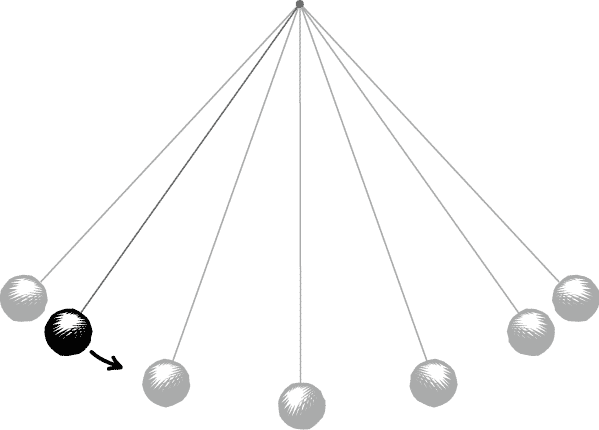
\includegraphics[width=0.8\linewidth]{Pictures/pendulum13}			
				\end{center}
			\end{column}	
			\begin{column}{.50\linewidth}
				\begin{center}
					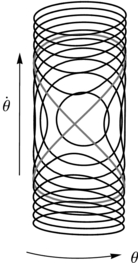
\includegraphics[width=0.45\linewidth]{Pictures/pendulum-phase-space}			
				\end{center}
			\end{column}	
		\end{columns}
		%
		\begin{defblock}[Symplectic Manifold]
			\includestandalone[width=0.95\textwidth]{Pictures/Figure_sym}	
		\end{defblock}
		%
		\begin{exblock}[$M = T^\ast Q$ is symplectic]
			$\omega = d \theta $ with
			$$ \left.\theta\right\vert_{(q,p)} (v) = p (\pi_\ast v) ~.$$
		\end{exblock}
	\end{column}
	\vrule{}
	\pause
	\begin{column}{.50\linewidth}
		\centering
		\textit{ "algebraic approach" to mechanics \dots}
		\vspace{1em}	
		\begin{defblock}[Classical Observables]
			Unital, associative, commutative algebra $C^\infty(M)$.
		\end{defblock}
		%
		\vspace{1em}
		\pause
		\begin{defblock}[Hamiltonian vector fields]
			$v_f \in \mathfrak{X}(M)$ such that:
			$$\iota_{v_f} \omega = -df \quad \text{(exact)}$$ %$\in B^1(M)$
			\small$v_f$ = \emph{Ham.v.f. pertaining to $f\in C^\infty(M)$}.
		\end{defblock}
		%
		\begin{defblock}[Poisson Algebra of Observables]
			$C^\infty(M)$ is a Poisson algebra with
			$$\{f,g\} = \iota_{v_g} \iota_{v_f} \omega = \omega(v_f,v_g) ~.$$
		\end{defblock}
	\end{column}
\end{columns}
\end{frame}
\note[itemize]{
	\footnotesize

	\item We work in the framework of multisymplectic geometry which is one of the possible generalizations of the well-established field of symplectic geometry.
	
	\item To recall what symplectic geometry is let me assume a particular point of view: mechanics.
	\\
	Idea:"
	Symplectic geometry is a branch of differential geometry studying symplectic manifolds; it originated as a formalization of the mathematical apparatus of classical mechanics and geometric optics."{\href{https://ncatlab.org/nlab/show/symplectic+geometry}{nlab}}
	
	Namely, a sym. mfd. is the geometric structure encoding the phase space of conservative, ordinary, classical, mechanical systems.
	
	\item $\theta$ = \emph{tautological 1-form}.
		$\theta$ evaluated at $p\in T^*Q$ in the fibre of $q\in Q$ and contracted with $v$ coincides with the form $p$ evaluated at $q$ and contracted with the push forward of $v$.
	
	\item We identify a special class of vector fields.
		Out of them one can define a Lie bracket.
	
	\item Poisson is a Lie algebra with the extra property of compatibility with the associative product (Leibniz rule)
}
%-------------------------------------------------------------------------------------------------------------------------------------------------

%------------------------------------------------------------------------------------------------
\begin{frame}{Syplectic geometry of the pendulum}\label{frame:symgeompendu}
  \begin{columns}[T]
   	\begin{column}{.35\textwidth}
   		\center
   		\vspace{-1em}
		\resizebox{.9\textwidth}{!}{
			\pgfmathtruncatemacro\steps{7}
			\pgfmathtruncatemacro\mintheta{-170}
			\pgfmathtruncatemacro\maxtheta{-30}
			\pgfmathsetmacro\deltatheta{(\maxtheta-\mintheta)/(\steps-1)}
			\pgfmathsetmacro\viewpitch{15}
			\pgfmathsetmacro\diam{2}
			\pgfmathsetmacro\H{2}
			\pgfmathsetmacro\deltaH{.5}
			\pgfmathsetmacro\X{\diam}
			\pgfmathsetmacro\Y{\diam*sin(\viewpitch)}	
			\pgfmathsetmacro\vel{\diam/4}	
					\begin{tikzpicture}
						\draw[green,dashed,fill=green!20] (0,0) ellipse ({\X} and {\Y});
						%\draw [blue,dashed] (-1.25,-3.5) arc (180:360:1.25 and -0.5);
						\draw[green,dashed,fill=green!20] (0,-{\H}) ellipse ({\X} and {\Y});
						\draw [blue,dashed] (-{\X},-{.5*\H}) arc (180:360:{\X} and -{\Y});
						\draw [green](-{\X},0) -- (-{\X},-{\H});
						\draw [green]({\X},-{\H}) -- ({\X},0);  
						\fill [green!80,opacity=0.5] (-{\X},0) -- (-{\X},-{\H}) arc (180:360:{\X} and {\Y}) -- ({\X},0) arc (0:180:{\X} and -{\Y});
						\draw [blue](-\X,-{.5*\H}) arc (180:360:{\X} and {\Y});

			\draw [black,-Latex](-\X,-{1.25*\H}) arc (180:355:{\X} and {\Y}) node[midway,below]{$\theta$};
			\draw [black,-Latex](-{1.25*\X},-{\H}) -- 
			node[left] {$p$}	 (-{1.25*\X},0);
					\end{tikzpicture}	
		}   	   	
   	
   	
   	
    \end{column}
    \begin{column}{.65\textwidth}	
		\begin{itemize}
			\item $M=T^\ast S^1\cong S^1\times \mathbb{R} \sim (\theta, p_\theta)$
			\item two coordinates charts
				\begin{itemize}
					\item[•] $\theta: M \to \mathbb{R}$\quad \emph{"configuration coordinate"}
					\item[•] $p: M \to \mathbb{R}$\quad \emph{"conjugate momentum"}
				\end{itemize}
			\item symplectic structure: $\omega = d \theta \wedge d p$.
		\end{itemize}
  	\end{column}
	\end{columns}			
	%
	\pause
	
	\begin{exblock}[Momentum observable]
  	\begin{columns}[T]
   	\begin{column}{.35\textwidth}
		\center
		\resizebox{.9\textwidth}{!}{
			\pgfmathtruncatemacro\steps{7}
			\pgfmathtruncatemacro\mintheta{-170}
			\pgfmathtruncatemacro\maxtheta{-30}
			\pgfmathsetmacro\deltatheta{(\maxtheta-\mintheta)/(\steps-1)}
			\pgfmathsetmacro\viewpitch{5}
			\pgfmathsetmacro\diam{4}
			\pgfmathsetmacro\H{4}
			\pgfmathsetmacro\deltaH{.5}
			\pgfmathsetmacro\X{\diam}
			\pgfmathsetmacro\Y{\diam*sin(\viewpitch)}	
			\pgfmathsetmacro\vel{\diam/4}	
					\begin{tikzpicture}
						\draw[green,dashed,fill=green!20] (0,0) ellipse ({\X} and {\Y});
						%\draw [blue,dashed] (-1.25,-3.5) arc (180:360:1.25 and -0.5);
						\draw[green,dashed,fill=green!20] (0,-{\H}) ellipse ({\X} and {\Y});
						\draw [blue,dashed] (-{\X},-{.5*\H}) arc (180:360:{\X} and -{\Y});
						\draw [green](-{\X},0) -- (-{\X},-{\H});
						\draw [green]({\X},-{\H}) -- ({\X},0);  
						\fill [green!80,opacity=0.5] (-{\X},0) -- (-{\X},-{\H}) arc (180:360:{\X} and {\Y}) -- ({\X},0) arc (0:180:{\X} and -{\Y});
						\draw [blue](-\X,-{.5*\H}) arc (180:360:{\X} and {\Y});

									\foreach \i in {0,1,...,\steps}{
								\pgfmathsetmacro\theta{\mintheta + \i*\deltatheta}
								\foreach \h in {0,-\deltaH,...,-\H}{
									\draw[red,-stealth] (0,\h)++({cos(\theta)*\X},{sin(\theta)*\Y}) --++({-\vel*sin(\theta)},{\vel*cos(\theta)*sin(\viewpitch)});

									}
						}							
					\end{tikzpicture}	
		}   	
    \end{column}
    \begin{column}{.65\textwidth}	
		\begin{itemize}
			\item The corresponding Ham. vector field $X_{p}= a ~\partial_\theta + b ~\partial_p$ satisfies
				\vspace{-1em}
				$$ d p = \iota_{X_p} \omega = a ~d p - b ~d \theta$$
			\item Flow of $X_p = \partial \theta$ are free rotations around the pivot
		\end{itemize}
  	\end{column}
	\end{columns}			
	\end{exblock}

	\pause

	\begin{exblock}[Energy observable]
  	\begin{columns}[T]
   	\begin{column}{.35\textwidth}
		\center
			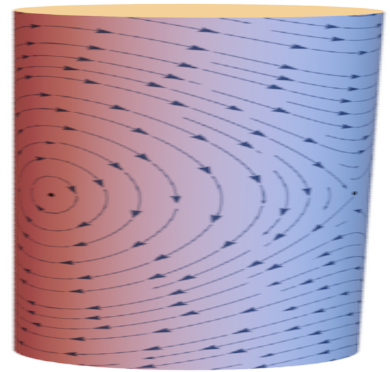
\includegraphics[width=.5\textwidth]{Pictures/pendulum_ham_PhaseSpace} 
		%https://mathematica.stackexchange.com/questions/64407/phase-portrait-on-a-cylinder
    \end{column}
    \begin{column}{.65\textwidth}	
		\begin{itemize}
			\item Interaction with the gravitational pull gives
				\vspace{-1em}			
				$$ H = \dfrac{p^2}{2 m \ell^2} + m	g \ell ( 1- \cos(\theta))$$
			\item 
				The corresponding Ham. v. f. results
				\vspace{-1em}				
				$$ X_H = - m g \ell \sin(\theta) \partial_p + \dfrac{p}{m \ell^2} \partial_\theta$$		
		\end{itemize}
  	\end{column}
	\end{columns}			
	\end{exblock}
	

\end{frame}
\note[itemize]{
	\item 	Recall: angular momentum $ p = m \ell \dot{\theta}$.
	\item Computing the flow of the Ham v.f. is where the analisys (exact solutions) or the numerics (approximate solutions) kicks in.
	\item why one should introduce all this machinery instead of going straight to the solution of the differential equations of motions?
		\begin{itemize}
			\item in quantization the global geometry of the system is more important then the local description of the classical motion
			\item efficient numerical schemes take in account the preservation of the symplectic form (do not solve the pde blindly but consider its geo-mech origin).
		\end{itemize}
}
%------------------------------------------------------------------------------------------------



\end{document}

%-------------------------------------------------------------------------------------------------------------------------------------------------
\section{Symmetries}
\checkpoint	
%-------------------------------------------------------------------------------------------------------------------------------------------------
\subsection{Hamiltonian action}
%\subsection{reduction}
	%+----------------------------------------------------------------------------+
%| SLIDES: 
%| Chapter: Hamiltonian symmetries
%| Author: Antonio miti
%| Event: Phd Colloquium - What is ... Geometric mechanics?
%+----------------------------------------------------------------------------+

%- HandOut Flag -----------------------------------------------------------------------------------------
\makeatletter
\@ifundefined{ifHandout}{%
  \expandafter\newif\csname ifHandout\endcsname
}{}
\makeatother

%- D0cum3nt ----------------------------------------------------------------------------------------------
\documentclass[beamer,10pt]{standalone}   
%\documentclass[beamer,10pt,handout]{standalone}  \Handouttrue  

\ifHandout
	\setbeameroption{show notes} %print notes   
\fi

	
%- Packages ----------------------------------------------------------------------------------------------
\usepackage{custom-style}
\usetikzlibrary{positioning}
\usepackage{multicol}


%--Beamer Style-----------------------------------------------------------------------------------------------
\usetheme{toninus}
\usepackage{animate}
\usetikzlibrary{positioning, arrows}
\usetikzlibrary{shapes}
\usetikzlibrary{calc}
\usetikzlibrary{backgrounds}
  \tikzset{
    invisible/.style={opacity=0},
    visible on/.style={alt=#1{}{invisible}},
    alt/.code args={<#1>#2#3}{%
      \alt<#1>{\pgfkeysalso{#2}}{\pgfkeysalso{#3}} % \pgfkeysalso doesn't change the path
    },
  }
 \usetikzlibrary{shapes.misc} 

  
  
\begin{document}

%-------------------------------------------------------------------------------------------------------------------------------------------------
\begin{frame}[t]{Symmetries: intuition}
	\begin{itemize}
		\item (elementary) symmetry: property of a geometric figure (shape) to be invariant under certain transformations.
	\end{itemize}
	\vfill
	\begin{center}
		\resizebox{\textwidth}{!}{			
			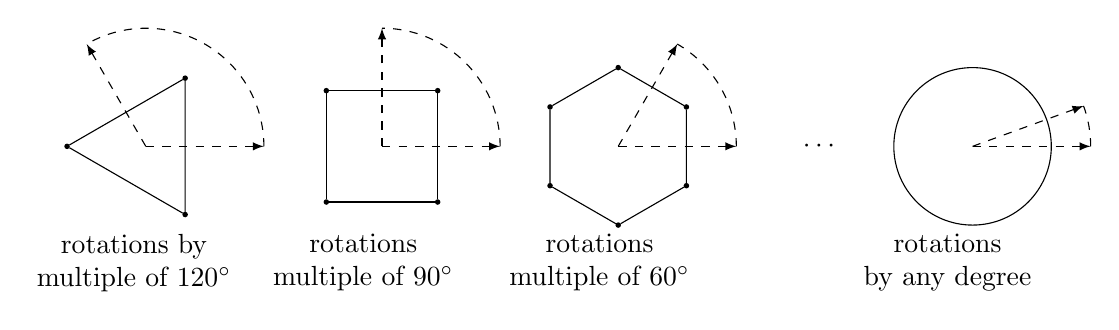
\begin{tikzpicture}
				\pgfmathtruncatemacro\R{1};
				\pgfmathsetmacro\Rext{1.5};
				\pgfmathsetmacro\dist{2*\Rext};
			    \draw[draw=none] (-\Rext,-1) rectangle (\Rext,\Rext);
		
				% Triangle
				\coordinate (o1) at (0,0);
				\draw[draw=none] (o1) -- (60:\R) node[circle, fill, minimum size=2pt,inner sep=0pt, outer sep=0pt](t1){};
				\draw[draw=none] (o1) -- (180:\R) node[circle, fill, minimum size=2pt,inner sep=0pt, outer sep=0pt](t2){};
				\draw[draw=none] (o1) -- (-60:\R) node[circle, fill, minimum size=2pt,inner sep=0pt, outer sep=0pt](t3){};
					
				\draw[dashed,-latex] (o1) -- (0:\Rext);
				\draw[dashed,-latex] (o1) -- (120:\Rext);
				\draw[dashed] (0:\Rext) arc(0:120:\Rext);
								
				\draw (t1) -- (t2) -- (t3) -- (t1);
				
				\node[below right,align=center,thick,outer sep=0pt,visible on=<2->] at (-\Rext,-1)
       				{rotations by\\ multiple of $120^\circ$};


				% Square	
				\coordinate (o2) at (\dist,0);
				\draw[draw=none] (o2) -- ++ (45:\R) node[circle, fill, minimum size=2pt,inner sep=0pt, outer sep=0pt](s1){};
				\draw[draw=none] (o2) -- ++ (135:\R) node[circle, fill, minimum size=2pt,inner sep=0pt, outer sep=0pt](s2){};
				\draw[draw=none] (o2) -- ++ (225:\R) node[circle, fill, minimum size=2pt,inner sep=0pt, outer sep=0pt](s3){};
				\draw[draw=none] (o2) -- ++ (315:\R) node[circle, fill, minimum size=2pt,inner sep=0pt, outer sep=0pt](s4){};
		
					
				\draw[dashed,-latex] (o2) -- ++ (0:\Rext);
				\draw[dashed,-latex] (o2) -- ++ (90:\Rext);
				\draw[dashed] (o2)++(0:\Rext) arc (0:90:\Rext);
								
				\draw (s1) -- (s2) -- (s3) -- (s4) -- (s1);	

				\node[below right,align=center,thick,outer sep=0pt,visible on=<2->] at (-\Rext+\dist,-1)
       				{rotations \\ multiple of $90^\circ$};

				%pentagon
				\coordinate (o3) at (2*\dist,0);
				\draw[draw=none] (o3) -- ++ (30:\R) node[circle, fill, minimum size=2pt,inner sep=0pt, outer sep=0pt](h1){};
				\draw[draw=none] (o3) -- ++ (90:\R) node[circle, fill, minimum size=2pt,inner sep=0pt, outer sep=0pt](h2){};
				\draw[draw=none] (o3) -- ++ (150:\R) node[circle, fill, minimum size=2pt,inner sep=0pt, outer sep=0pt](h3){};
				\draw[draw=none] (o3) -- ++ (210:\R) node[circle, fill, minimum size=2pt,inner sep=0pt, outer sep=0pt](h4){};
				\draw[draw=none] (o3) -- ++ (270:\R) node[circle, fill, minimum size=2pt,inner sep=0pt, outer sep=0pt](h5){};
				\draw[draw=none] (o3) -- ++ (330:\R) node[circle, fill, minimum size=2pt,inner sep=0pt, outer sep=0pt](h6){};
		
		
				\draw[dashed,-latex] (o3) -- ++ (0:\Rext);
				\draw[dashed,-latex] (o3) -- ++ (60:\Rext);
				\draw[dashed] (o3)++(0:\Rext) arc (0:60:\Rext);
								
				\draw (h1) -- (h2) -- (h3) -- (h4)-- (h5) -- (h6) -- (h1);				
				
				\node[below right,align=center,thick,outer sep=0pt,visible on=<2->] at (-\Rext+2*\dist,-1)
       				{rotations \\ multiple of $60^\circ$};
       				
       			\node[] at (2.85*\dist,0) {$\cdots$};				

				\coordinate (o4) at (3.5*\dist,0);			
				\draw[,visible on=<3->] (o4) circle (1);
				\draw[dashed,-latex,visible on=<3->] (o4) -- ++ (0:\Rext);
				\draw[dashed,-latex,visible on=<3->] (o4) -- ++ (20:\Rext);
				\draw[dashed,visible on=<3->] (o4)++(0:\Rext) arc(0:20:\Rext);
				\node[below right,align=center,thick,outer sep=0pt,visible on=<3->] at (-\Rext+3.5*\dist,-1)
       				{rotations \\ by any degree};				
			
			\end{tikzpicture}	
		}
	\end{center}
	\vfill
	\begin{itemize}
		\item<2-> 	Intuitive notion of symmetry is discrete.
		\item<3-> 	Mechanical systems possess "continuous" symmetries.
					\vfill
					\alert{ Keyword: Lie Groups.}
	\end{itemize}
	
\end{frame}
\note[itemize]{
\item Up to now we showed how basic mechanics structures can be encoded by geometry.
\item There is another complementary geometrical property naturally appearing in physics: symmetry.
	\item in contrast to the intuitive notion of symmetries that might come to one's mind (discrete) - like the mirror symmetry of a butterfly or the radial symmetry of flowers- mechanical systems has continuous symmetries.
	\item e.g. pendulum has rotation symmetries.
}
%-------------------------------------------------------------------------------------------------------------------------------------------------

%-------------------------------------------------------------------------------------------------------------------------------------------------
\begin{frame}[t]{Symmetries: Geometric mechanics}
	\begin{itemize}
		\item Consider a phase space $M$ (symplectic manifold) e.g. a Torus.
	\end{itemize}
	%
	\vfill
	\begin{columns}
    	\begin{column}{.5\textwidth}
			\center
			\ifHandout \else
				\includegraphics<1>[width=.75\textwidth]{Pictures/torus2}
				\includegraphics<2>[width=.75\textwidth]{Pictures/arnoldcat-frame/arnoldclown-0.png}
			\fi
				\only<3->{	
					\animategraphics[autoplay,palindrome,width=.75\textwidth]{2}{Pictures/arnoldcat-frame/arnoldclown-}{0}{3}
				}
		\end{column}
    	\begin{column}{.5\textwidth}
    		\only<2>{
	    		\emph{For the sake of representation,\\
	    		label each state with a color.
	    		\\
	    		e.g. glue a picture on the surface}
	    		\center
				
\includegraphics[width=.5\textwidth]{Pictures/clown.png}
			}
			\only<3->{
				Arnold's cat map
				\\
				\tiny
				\url{https://faculty.math.illinois.edu/~palmore/math351-n1/catmap.htm} 
			}
		\end{column}
	\end{columns}
	\vfill
	\onslide<3->{
	\begin{defblock}[Transformation]
		Smooth family of mappings from $M$ into itself.\\
		(Lie group smoothly acting on $M$)
	\end{defblock}
	}
	\vfill
	\onslide<4->{
	\begin{defblock}[Symmetry]
		Is a transformation preserving the symplectic structure of $M$.
	\end{defblock}	
	}

\end{frame}
\note[itemize]{
	\item Let's consider a symplectic manifold, e.g the torus (it is orientable and 2 dimensional, therefore a volume form is also symplectic)
	\item Observe: A transformation acts (transform) observables (via pullback) and hamiltonian vector field (via push forward)
	\item loosely speaking a "symmetry" is a transformation such that:
		given an observable $o$ with Ham. vec. field $x$, the Ham. vec. field $\bar{x}$ of the transformed observable $o'$ coincides with the transformation $x'$ of $x$.
	\item questo è un po' improrio, di solito si definisco trasformazioni canoniche le trasformazioni che preservano la struttura simplettica e simmetrie le trasformazioni canoniche che preservano anche la fissata hamiltoniana.
	\item formally symmetries are described by Lie group actions on configuration spaces or phase spaces.
	\item their importance lies in the associated conserved quantities and the reduced description that arise from them.

		
}
%-------------------------------------------------------------------------------------------------------------------------------------------------

%-------------------------------------------------------------------------------------------------------------------------------------------------
\begin{frame}[t]{Hamiltonian Symmetries: comomentum maps}
	\begin{block}{Recall: gist of the symplectic structure}
			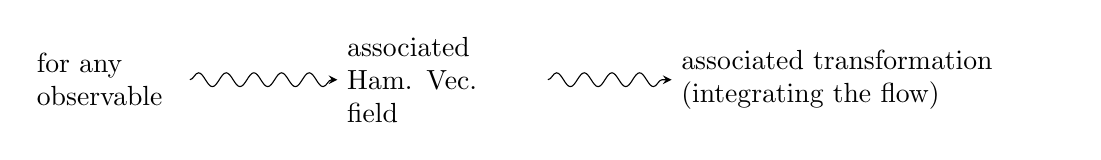
\begin{tikzpicture}[
				node distance=0.35\linewidth,
				]
				\node [text width=0.15\linewidth,rectangle] (lhs) {for any \\ observable};
				\node [text width=0.2\linewidth, rectangle,right of=lhs] (chs) {associated \\ Ham. Vec. field};
				\node [text width=0.4\linewidth, rectangle,right of=chs,node distance=.45\linewidth] (rhs) {associated transformation\\ (integrating the flow)};
				\draw[-stealth,decorate,decoration={snake}] (lhs) -- (chs);
				\draw[-stealth,decorate,decoration={snake}] (chs) -- (rhs);
			\end{tikzpicture}
	\end{block}
	%
	\vfill
	\onslide<2->{
		\begin{defblock}[Hamiltonian symmetry]
			Transformation obtainable as a flow of a certain observable quantity ("generalized momentum").
			\\
			Mathematically, existence of a certain function called \emph{comomentum map}.
		\end{defblock}
	}
	\vspace{-.5em}
	\begin{columns}
    	\begin{column}[t]{.5\textwidth}
			\only<3->{
			\begin{exblock}[Angular momentum $L$]
					\center
					\resizebox{.9\textwidth}{!}{
						\pgfmathtruncatemacro\steps{8}
						\pgfmathtruncatemacro\mintheta{-170}
						\pgfmathtruncatemacro\maxtheta{-90}
						\pgfmathsetmacro\deltatheta{(\maxtheta-\mintheta)/(\steps-1)}
						\pgfmathsetmacro\viewpitch{30}
						\pgfmathsetmacro\diam{2}
						\pgfmathsetmacro\H{4}
						\pgfmathsetmacro\deltaH{.5}
						\pgfmathsetmacro\X{\diam}
						\pgfmathsetmacro\Y{\diam*sin(\viewpitch)}	
						\pgfmathsetmacro\vel{\diam/4}	
						\begin{animateinline}[autoplay,loop]{6} % 5 fps, same as 0.2 s transduration
							\multiframe{\steps}{i=0+1}{
								\begin{tikzpicture}
									\pgfmathsetmacro\theta{\mintheta + \i*\deltatheta}
									\draw[green,dashed,fill=green!20] (0,0) ellipse ({\X} and {\Y});
									%\draw [blue,dashed] (-1.25,-3.5) arc (180:360:1.25 and -0.5);
									\draw[green,dashed,fill=green!20] (0,-{\H}) ellipse ({\X} and {\Y});
									\draw [blue,dashed] (-{\X},-{.5*\H}) arc (180:360:{\X} and -{\Y});
									\draw [green](-{\X},0) -- (-{\X},-{\H});
									\draw [green]({\X},-{\H}) -- ({\X},0);  
									\fill [green!80,opacity=0.5] (-{\X},0) -- (-{\X},-{\H}) arc (180:360:{\X} and {\Y}) -- ({\X},0) arc (0:180:{\X} and -{\Y});
									\draw [blue](-\X,-{.5*\H}) arc (180:360:{\X} and {\Y});
									\foreach \h in {0,-\deltaH,...,-\H}{
										\draw[red,-stealth] (0,\h)++({cos(\theta)*\X},{sin(\theta)*\Y}) --++({-\vel*sin(\theta)},{\vel*cos(\theta)*sin(\viewpitch)});
										\draw[red] ({cos(\theta)*\X},{sin(\theta)*\Y}) -- ({cos(\theta)*\X},{sin(\theta)*\Y-\H});
				
										
										\draw[red,-stealth] (0,\h)++({cos(\theta+90)*\X},{sin(\theta+90)*\Y}) --++({-\vel*sin(\theta+90)},{\vel*cos(\theta+90)*sin(\viewpitch)});
										\draw[red] ({cos(\theta+90)*\X},{sin(\theta+90)*\Y}) -- ({cos(\theta+90)*\X},{sin(\theta+90)*\Y-\H});
									}
								    \draw[->] (5,-{\H})--(5,0) node[above] {$\dot{\Theta}$}; % ordinate
								    \draw[->] (4,-{.5*\H})--(6,-{.5*\H})node[right] {$L$};%angular momentum; % ascisse
								    \draw[-,red] (4,-{\H})--(6,0); % l'axe des abscisses
								\end{tikzpicture}	
							}
						\end{animateinline}
					}
			\end{exblock}
			}
		\end{column}
		\pause		
    	\begin{column}[t]{.5\textwidth}
    		\onslide<4->{
				\begin{upshotblocktitle}[Crucial tool in Geo. Mec.]
					\center
					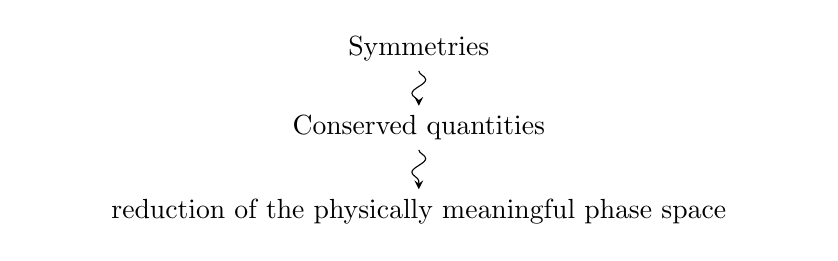
\begin{tikzpicture}[]
						\node [text width=0.8\linewidth,rectangle,align=center] (lhs) {Symmetries};
						\node [text width=0.8\linewidth, rectangle,below of=lhs,align=center] (chs) {Conserved quantities};
						\node [text width=0.8\linewidth, rectangle,below= 0.5 of chs,align=center] (rhs) {reduction of the physically meaningful phase space};
						\draw[-stealth,decorate,decoration={snake}] (lhs) -- (chs);
						\draw[-stealth,decorate,decoration={snake}] (chs) -- (rhs);
					\end{tikzpicture}						
				\end{upshotblocktitle}    	
			}
		\end{column}	
	
	\end{columns}




\end{frame}
\note[itemize]{
	\item among all possible symmetries there's a special class
	\item slogan:		Hamiltonian symmetry $\Leftrightarrow$ Admits a comoment map
	\item comomentum maps are one of the most powerful tools in the geometric mechanics toolbox
	
}
%-------------------------------------------------------------------------------------------------------------------------------------------------

%
%\begin{frame}
%						\begin{tikzpicture}
%							\pgfmathsetmacro\theta{-120}
%							\pgfmathsetmacro\viewpitch{30}
%							\pgfmathsetmacro\diam{2}
%							\pgfmathsetmacro\H{4}
%							\pgfmathsetmacro\deltaH{.5}
%							\pgfmathsetmacro\X{\diam}
%							\pgfmathsetmacro\Y{\diam*sin(\viewpitch)}	
%							\pgfmathsetmacro\vel{\diam/4}	
%													
%							
%							\draw[green,dashed,fill=green!20] (0,0) ellipse ({\X} and {\Y});
%							%\draw [blue,dashed] (-1.25,-3.5) arc (180:360:1.25 and -0.5);
%							\draw[green,dashed,fill=green!20] (0,-{\H}) ellipse ({\X} and {\Y});
%							\draw [blue,dashed] (-{\X},-{.5*\H}) arc (180:360:{\X} and -{\Y});
%		
%							\draw [green](-{\X},0) -- (-{\X},-{\H});
%							\draw [green]({\X},-{\H}) -- ({\X},0);  
%							\fill [green!80,opacity=0.5] (-{\X},0) -- (-{\X},-{\H}) arc (180:360:{\X} and {\Y}) -- ({\X},0) arc (0:180:{\X} and -{\Y});
%		
%							\draw [blue](-\X,-{.5*\H}) arc (180:360:{\X} and {\Y});
%		
%							\foreach \h in {0,-\deltaH,...,-\H}{
%								\coordinate (p) at (0,\h)++({cos(\theta)*\X},{sin(\theta)*\Y});
%								%\fill[blue] (0,\h)++({cos(\theta)*\X},{sin(\theta)*\Y}) circle(2pt);
%								\draw[red,-stealth] (0,\h)++({cos(\theta)*\X},{sin(\theta)*\Y}) --++({-\vel*sin(\theta)},{\vel*cos(\theta)*sin(\viewpitch)});
%								\draw[red] ({cos(\theta)*\X},{sin(\theta)*\Y}) -- ({cos(\theta)*\X},{sin(\theta)*\Y-\H});
%		
%						}
%		
%					    \draw[->] (5,-{\H})--(5,0) node[above] {$\dot{\Theta}$}; % ordinate
%					    \draw[->] (4,-{.5*\H})--(6,-{.5*\H})node[right] {$L$}; % ascisse
%					    \draw[-,red] (4,-{\H})--(6,0); % l'axe des abscisses
%		
%					\end{tikzpicture}		
%
%\end{frame}

%------------------------------------------------------------------------------------------------
% Frame inspired by Leonid: passing from moment maps to comoment maps
\begin{frame}[fragile]{Details: Moment maps in symplectic geometry}
	Let $(M,\omega)$ be a symplectic manifold, $\vartheta: G\times M \to M$ a Lie group action preserving $\omega$ and $v:\mathfrak{g}\to \mathfrak{X}(M)$ the corresponding infinitesimal action
	%
		\begin{defblock}[Moment map pertaining to $\vartheta$]
			Smooth map $ \mu: M \to \mathfrak{g}^\ast$ such that: \stackunder{$d \langle\mu , \xi \rangle = \iota_{v_\xi}\omega \scriptstyle\quad \forall \xi \in \mathfrak{g}$}{$f (\vartheta_g(x)) = Ad^\ast_g (f(x)) \scriptstyle\quad \forall g \in G, x \in M$}
		\end{defblock}
	%
	\vfill
	\pause
	\emph{... from a dual perspective (assuming $G$ connected) ...}
	\vspace*{-.5em}
			\begin{defblock}[Comoment map pertaining to $v$]
				\begin{columns}
					\begin{column}{.5\linewidth}	
			Lie algebra morphism \qquad $ f: \mathfrak{g} \to C^\infty(M) $
			\\
			such that \qquad $ d~f (x) = -\iota_{v_x} \omega \qquad \forall x \in \mathfrak{g}~.$
					\end{column}
					\begin{column}{.4\linewidth}	
						\begin{displaymath}
							\begin{tikzcd}
								& C^{\infty}(M,\omega) \ar[d]
								\\
								\mathfrak{g} \ar[ur,dashed,"(f)"]\ar[r,"v"']& \mathfrak{X}(M)
							\end{tikzcd}	
						\end{displaymath}
					\end{column}
				\end{columns}
		\end{defblock}		
	%
	\vfill
	\pause
	\emph{... a tool encoding conserved quantities ...}
	\vspace*{-.5em}
	\begin{propblock}[Noether Theorem]
		\small Fixed $H\in C^\infty_{\text{Ham}}(M)$ ($\mathfrak{g}$-invariant) ,
				\qquad
				$\mathcal{L}_{v_H} f(x) = 0 \qquad \forall x \in \mathfrak{g}~.$
	\end{propblock}
\end{frame}
\note[itemize]{
	\item comoment map is a Lie algebra morphism projecting to $v$. (Triangle diagram in Lie algebra category).
}
%------------------------------------------------------------------------------------------------


\end{document}



%-------------------------------------------------------------------------------------------------------------------------------------------------
\section{Going Higher}
\checkpoint	
%-------------------------------------------------------------------------------------------------------------------------------------------------
	%+----------------------------------------------------------------------------+
%| SLIDES: 
%| Chapter: Brief introduction to multisymplectic geometry and Homotopy momap
%| Author: Antonio miti
%| Event: PHD preliminary Defence
%+----------------------------------------------------------------------------+

%- HandOut Flag -----------------------------------------------------------------------------------------
\newif\ifHandout

%- D0cum3nt ----------------------------------------------------------------------------------------------
\documentclass[beamer,10pt]{standalone}   
%\documentclass[beamer,10pt,handout]{standalone}  \Handouttrue  

%- HandOut Flag -----------------------------------------------------------------------------------------
\ifHandout
	\setbeameroption{show notes} %print notes   
\fi

	
%- Packages ----------------------------------------------------------------------------------------------
\usepackage{custom-style}




%--Beamer Style-----------------------------------------------------------------------------------------------
\usetheme{toninus}
\usetikzlibrary{positioning}




%---------------------------------------------------------------------------------------------------------------------------------------------------
%- D0cum3nt ----------------------------------------------------------------------------------------------------------------------------------
\begin{document}
%------------------------------------------------------------------------------------------------


%-------------------------------------------------------------------------------------------------------------------------------------------------
\begin{frame}[t]{Geometric Mechanics: Take Away Message}
	\begin{itemize}
		\item[•] \alert{States} are encoded by a \alert{symplectic manifold}.
		\begin{itemize}
			\item[-] Smooth manifolds arise naturally in the description of mechanical systems.
			\item[-] Constraints can be enforced intrinsically
			\item[-] Geo. Mech. yields an inherent intuition of diff. geom. structures.
		\end{itemize}
		\item<2->[•] \alert{Observables} quantities are encoded by \alert{smooth functions}.
		\begin{itemize}
			\item[-] The symplectic structure prescribe how to associate a vec. field to any observable.
			\item[-] Time evolution is obtained by integrating the flow along an Ham. v.f.
		\end{itemize}				
		\item<3->[•] \alert{Continuous symmetries} are encoded by \alert{symplectic Lie group actions}.
		\begin{itemize}
			\item[-] A relevant class of symmetries can be reconstructed from observables quantities via \emph{comomentum maps}.
			\item[-] Their importance lies in the existence of corresponding conserved quantities and the reduced description arising from them.
		\end{itemize}				
	\end{itemize}
	%Symplectic geometry is central
	\vfill
	%
	\onslide<4->{
		\begin{disclaimerbox}[we glossed on some technical details]
			\resizebox{.85\textwidth}{!}{
				\begin{columns}
					\begin{column}[T]{0.65\textwidth}
						\begin{itemize}
							\item[-] \color{black!80!white} Galilean / Special / General relativity (observer)
							\item[-] Holonomics / Non-holonomics constraints
							\item[-] Conservative / Dissipative system
							\item[-] Discrete / \alert{Continuous} degrees of freedom.
						\end{itemize}
					\end{column}					
					\begin{column}[T]{0.5\textwidth}
						\begin{itemize}
							\item[-] \color{black!80!white} Classical / Quantum observability
							\item[-] Lagrangian / Hamiltonian dynamics
							\item[-] Velocities $\neq$ Momenta
							\item[-] Local / Global flow integrability
						\end{itemize}
					\end{column}							
				\end{columns}
			}				
		\end{disclaimerbox}	
	}

\end{frame}
\note[itemize]{
	\item è centrale nel senso che è l'arena  in cui descrivere molti sistemi ideali
	\item richiede estensioni e generalizzazioni per codificare casi di studio piu' realistici e/o generali

	\item geometry is an intrisic part of mechanics. 
	The set of configurations has a natural geometric structure, constraints are automatically satisfied by this choice.
	\item {\bf descibing states as points of a manifold is the principal premise of geometric mechanics.}
	\item Conf. space and Phase space are manifolds (higher dimensional generalization of surfaces)
	\item A large class of constraints can be enforced intrinsically by the topology (shape) of the manifold.


	\item an important trait of geometric mechanics is its intuitive nature: structures and time evolution of mechanical systems can be illustrated by visualizing configuration and phase space.
	Practilly working in Geo. Mech. often means to exploit the inherent geometric intuition.
	
	\item an important characteristic is its emphasis on laying a rigourous mathematical foundation on which one can build upon mechanics. 
	While Newtonian mechanics is highly desciptive it does not reveal the underlying structure.
	In geo. mech. computations are structural arguments which provide insight into the frabic they represent. 

	\item Huge disclaimer, in the above presentation we glossed out on many details...

}

%-------------------------------------------------------------------------------------------------------------------------------------------------




%-------------------------------------------------------------------------------------------------------------------------------------------------
\begin{frame}[t,fragile]{Going higher: multisymplectic geometry}
	\begin{block}{Historical motivation}
		Mechanics: geometrical foundations of \textit{(first-order)} field theories.
	\end{block}
	\vfill	
	\begin{table}
		\only<2->{
		\begin{tabular}{|p{0.2\textwidth}|p{0.3\textwidth}|p{0.35\textwidth}|} 
            \hline
            \parbox[][20pt][c]{0.2\textwidth}{mechanics} & \multicolumn{2}{c|}{geometry} \\
            \hline
            \parbox[][20pt][c]{0.2\textwidth}{phase space} & symplectic manifold & \only<3->{multisymplectic manifold} \\[.25em]
            \parbox[][20pt][c]{0.2\textwidth}{classical \\ observables} & Poisson algebra & \only<3->{$L_\infty$-algebra} \\[.25em]
            \parbox[][20pt][c]{0.2\textwidth}{symmetries} &  group actions admitting comoment map & 
            \only<3->{group actions admitting 
				\tikz[baseline,remember picture]{\node[rounded corners,
	                        fill=orange!10,draw=orange!30,anchor=base]            
	            			(target) {homotopy comomentum map};
	            }
            }
            \\
            \hline
  \multicolumn{1}{c}{}
            &  
            \multicolumn{1}{@{}c@{}}{$\underbrace{\hspace*{.3\textwidth}}_{\text{point-like particles systems}}$} 
            &
            \multicolumn{1}{@{}c@{}}{\only<4->{$\underbrace{\hspace*{.3\textwidth}}_{\text{field-theoretic systems}}$}} 
		\end{tabular}
		}
	\end{table}		
	\vfill
	\onslide<4->{
		\begin{block}{Scope of the thesis}
			\begin{itemize}
				\item[$\bullet$] Develop theory of 
					\tikz[baseline,remember picture]{\node[rounded corners,
	                        fill=orange!10,draw=orange!30,anchor=base]            
	            			(base) {homotopy comomentum maps};
	            	}
	            \item[$\bullet$] produce new meaningful examples.
			\end{itemize}
		\end{block}
		%
        \begin{tikzpicture}[overlay,remember picture]
			\path[->]<4-> (base.east) edge[bend right](target.south east);
		\end{tikzpicture}
	}
	%
\end{frame}
\note[itemize]{
	\item Historically, the interest in multisymplectic manifolds, has been motivated by the need for understanding the geometrical foundations of first-order classical field theories.
	The key point is that, just as one can associate a symplectic manifold to an ordinary classical mechanical system (e.g. a single
point-like particle constrained to some manifold), it is possible to associate a multisymplectic
manifold to any classical field system (e.g. a continuous medium like a filament or a fluid). See frame Extra-\ref{Frame:Ms-Field-Mechanics} 
	
	\item General ideas basic parallelisms with caveats
	\item caveat: points in multiphase spaces are not states
	\item the table hides the duality between geometric and algebraic approaches to the problem.
	\item 
}
%-------------------------------------------------------------------------------------------------------------------------------------------------












%----------------------------------------------------------------------------------------------------------------------------------
\end{document}
%----------------------------------------------------------------------------------------------------------------------------------











	\thankyouslide

%------------------------------------------------------------------------------------------------

%------------------------------------------------------------------------------------------------




%------------------------------------------------------------------------------------------------
% APPENDIX
%------------------------------------------------------------------------------------------------
\appendix
%-------------------------------------------------------------------------------------------------------------------------------------------------
\section{Complementary Material}
	%+----------------------------------------------------------------------------+
%| SLIDES: 
%| Chapter: Complementary material - details on eventual questions
%| Author: Antonio miti
%| Event: PHD preliminary Defence
%+----------------------------------------------------------------------------+
%- HandOut Flag -----------------------------------------------------------------------------------------
\makeatletter
\@ifundefined{ifHandout}{%
  \expandafter\newif\csname ifHandout\endcsname
}{}
\makeatother

%- D0cum3nt ----------------------------------------------------------------------------------------------
\documentclass[beamer,10pt]{standalone}   
%\documentclass[beamer,10pt,handout]{standalone}  \Handouttrue  

\ifHandout
	\setbeameroption{show notes} %print notes   
\fi

	
%- Packages ----------------------------------------------------------------------------------------------
\usepackage{custom-style}

%--Beamer Style-----------------------------------------------------------------------------------------------
\usetheme{toninus}



\providecommand{\blank}{\text{\textvisiblespace}}


\newcommand{\subsectiontitle}{
  \begin{frame}
  \vfill
  \centering
  \begin{beamercolorbox}[sep=8pt,center,shadow=true,rounded=true]{title}
    \usebeamerfont{title}\insertsectionhead\par%
    \usebeamerfont{title}\insertsubsectionhead\par%
  \end{beamercolorbox}
  \vfill
  \end{frame}
}

\providecommand{\blank}{\text{\textvisiblespace}}




%---------------------------------------------------------------------------------------------------------------------------------------------------
%- D0cum3nt ----------------------------------------------------------------------------------------------------------------------------------
\begin{document}
%------------------------------------------------------------------------------------------------

%##################################################################################
\begin{frame}
	\begin{center}
	\Huge\emph{Supplementary Material}
	\end{center}
\end{frame}
\note[itemize]{
	\item
}
\addtocounter{framenumber}{-1}
%##################################################################################





%===================================================================================
\section{Background}
%===================================================================================



%-------------------------------------------------------------------------------------------------------------------------------------------------
\subsection{Symplectic Manifolds}
%-------------------------------------------------------------------------------------------------------------------------------------------------


%------------------------------------------------------------------------------------------------
\begin{frame}{Geometry of symmetries}\label{frame:geometrysymmetries}
	Basic mechanical structures are encoded in geometry. but there is another complementary geometrical property that's natural in physics: symmetry!
	\begin{alertblock}{Upshot}
		Continous symmetries are described by actions of a Lie group on $M$.
	\end{alertblock}
	\begin{block}{Noether}
		Presence of symmetries $\quad \Rightarrow \quad$ existence of conserved quantities.
	\end{block}	
	\begin{block}{Key concept:}
		Noether current are encoded in a \emph{moment map}  $\mu :M \rightarrow \mathfrak{g}^*$ (the dual of the comoment map $f$. 
	\end{block}
  \begin{columns}[T]
   	\begin{column}{.6\textwidth}
			\begin{block}{Symplectic reduction:}
			\begin{itemize}
				\item System dynamics should be restricted to level set of conserved observables in order to efficiently store dynamical properties.
				\item Under certain assumptions, $\mu^{-1}( 0 )/G$ is a symplectic manifold with an "induced" symplectic structure.
			\end{itemize}
			\end{block}
    \end{column}
    \begin{column}{.4\textwidth}	
			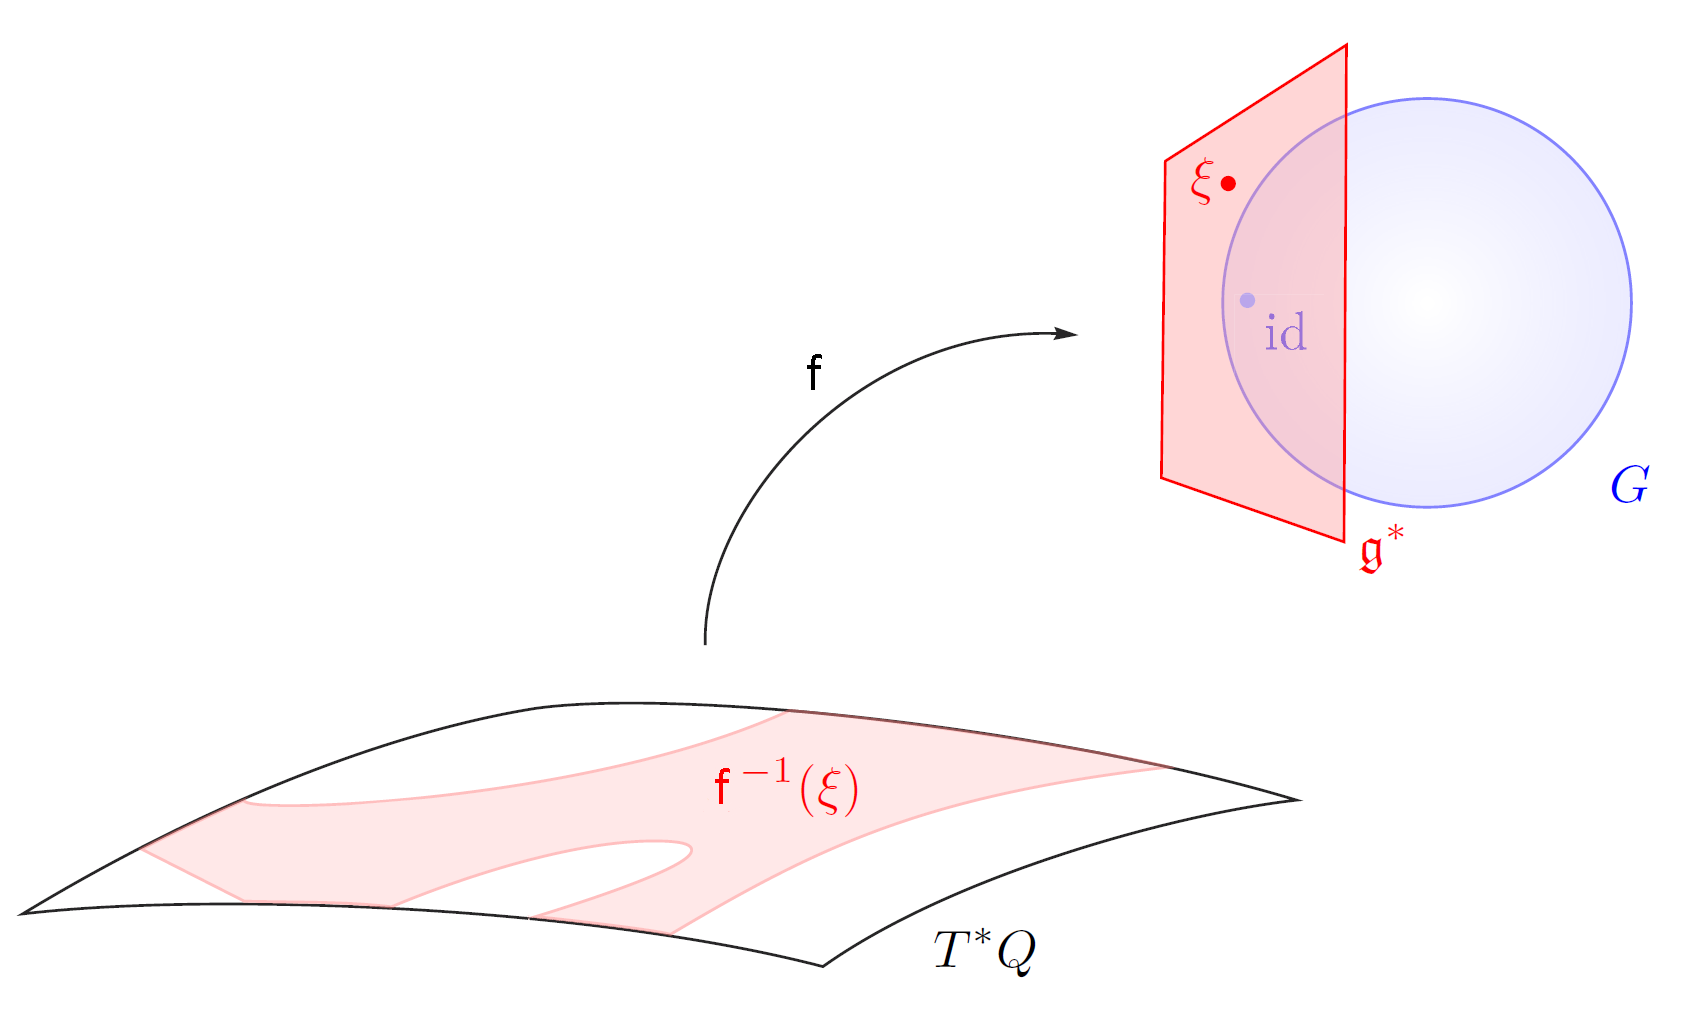
\includegraphics[width=\textwidth]{Pictures/Reduction} 
  	\end{column}
	\end{columns}			
\end{frame}
\note[itemize]{
	\item
}
%------------------------------------------------------------------------------------------------

%----------------------------------------------------------------------------------------------------------------------------------
\begin{frame}[fragile]{Configuration Space}
  	\begin{columns}[T]
    	\begin{column}{.5\textwidth}		
			\includegraphics<1>[width=\textwidth]{Pictures/GeoMec}
			\includegraphics<2->[width=\textwidth]{Pictures/GeoMec_noted}
    	\end{column}
    	\begin{column}{.5\textwidth}
			\begin{displaymath}				
   				Q \coloneqq
   				\left\{
				\parbox{45mm}{All possible admissible spatial displacements of a system.}
				 \right\}.
			\end{displaymath}

			\begin{block}<2->{Assumption 1:}
				For point particle $Q$ is a submanifold of $\mathbb{R}^n$.
			\end{block}

			\begin{block}<3->{Assumption 2:}
				Constraints are intrinsically encoded in the geometric structure of $Q$.
			\end{block}

			\vfill
			\begin{alertblock}<4->{Upshot:}
				$Q$ is a \emph{smooth manifold}. 
				Configuration of a system are naturally described by points on it. Configuration coordinates are charts.
			\end{alertblock}
    	\end{column}
  	\end{columns}	
\end{frame}
\note[itemize]{
	\item Consider the set of all possible admissible spatial displacements of a system.
}
%----------------------------------------------------------------------------------------------------------------------------------



%----------------------------------------------------------------------------------------------------------------------------------
\begin{frame}[t]{Symplectic Geometry}
	\begin{exampleblock}{Key point}
		$T^\ast Q$ it's naturally symplectic (i.e. endowed with a closed, bilinear, skew-symmetric form).
		\\
		\underline{Abstraction}: Mechanical systems $\quad \mapsto \quad$ symplectic manifold $(M,\omega)$.
	\end{exampleblock}
	%
	\vfill
  	\begin{columns}[T]
    	\begin{column}{.5\textwidth}	
			\includegraphics<1>[width=1.1\textwidth]{Pictures/Fig7} 
			\includegraphics<2->[width=1.1\textwidth]{Pictures/Fig8} 		
    	\end{column}
    	\begin{column}{.5\textwidth}
			\begin{itemize}
				\item<1-> Classical observables are elements in $C^\infty(M,\mathbb{R})$
				\item<2-> Observable yields hamiltonian fields $\textrm{d} H = \omega(X_H, \cdot)$
				\item<3-> Trajectories are integral flows of $X_H$
			\end{itemize}
    	\end{column}
  	\end{columns}				
	%
\end{frame}
\note[itemize]{
	\item

}
%----------------------------------------------------------------------------------------------------------------------------------

	\begin{frame}{Trajectories}
  	\begin{columns}[T]
    	\begin{column}{.5\textwidth}		
				\begin{center}
					Double Pendulum:
  	  				\includegraphics<1->[width=\textwidth]{Pics/Fig4} 
    				\vspace{3em}
    				General system:
					\includegraphics<1->[width=\textwidth]{Pics/Fig2} 	
				\end{center}
    	\end{column}
    	\begin{column}{.5\textwidth}


 				\begin{alertblock}<2->{Upshot}
 					 Trajectories of the system can be described by smooth parametrized curves on $Q$
 					\begin{displaymath}
 						Conf = C^\infty(\mathbb{R},Q)
 					\end{displaymath}
 				\end{alertblock}
 					\vspace{1em}

					
    	\end{column}
  	\end{columns}	
	\end{frame}

	\begin{frame}{Velocities}
  	\begin{columns}[T]
    	\begin{column}{.5\textwidth}		
				\begin{center}
					Double Pendulum:
  	  				\includegraphics<1->[width=\textwidth]{Pics/Fig5} 
    				\vspace{3em}
    				General system:
					\includegraphics<1->[width=\textwidth]{Pics/Fig3} 	
				\end{center}
    	\end{column}
    	\begin{column}{.5\textwidth}


 				\begin{alertblock}<2->{Upshot}
 					Instant velocities along a trajectory are \emph{tangent vectors} to the manifold $Q$
 					\begin{displaymath}
 						\dot{\gamma}(t) = V_{\gamma(t)} \in T_{\gamma(t)} Q
 					\end{displaymath}
 				\end{alertblock}
 				\begin{alertblock}<3->{Upshot}
					Collectively, all the possible tangent vector constitute another manifold called the \emph{Tangent Bundle}
					\begin{displaymath}
						TQ = \coprod_{q \in Q} T_q Q
					\end{displaymath}
 				\end{alertblock}
 					%\vspace{1em}
				\begin{center} 				
 					%\includegraphics<2->[width=\textwidth]{Pics/KinematicalConfig}		
 				\end{center}
    	\end{column}
  	\end{columns}	
	\end{frame}



%-------------------------------------------------------------------------------------------------------------------------------------------------
\subsection{MultiSymplectic Manifolds}
%-------------------------------------------------------------------------------------------------------------------------------------------------


%------------------------------------------------------------------------------------------------
\begin{frame}[fragile]{MS geometry and classical field mechanics}
		Consider a smooth manifold $Y$,
		\begin{columns}
			\hfill
			\begin{column}{.5\linewidth}
				\emph{Multicotangent bundle} $\bigwedge = \bigwedge^n T^\ast Y$\\
				is naturally $n$-plectic
			\end{column}
			\begin{column}{.4\linewidth}
				\[
				\begin{tikzcd}
					\Lambda \ar[d,"\pi"'] & T \Lambda \ar[d,"T \pi"] \ar[l] \\
					Y								& T Y \ar[l]
				\end{tikzcd}	
				\]
			\end{column}
		\end{columns}
	\pause
	\begin{defblock}[Tautological $n$-form]
		$\theta \in \Omega^n(\Lambda)$ such that:
		\begin{displaymath}
		\begin{split}
			\left[ \iota_{u_1 \wedge \ldots \wedge u_n} \theta \right]_\eta 
			&= \iota_{(T \pi)_\ast u_1 \wedge \ldots \wedge (T \pi)_\ast u_n} \eta \\
			&= \iota_{u_1 \wedge \ldots \wedge u_n} \pi^\ast \eta 
			\qquad \qquad \forall \eta \in \Lambda \, , \: \forall u_i \in T_\eta \Lambda 		
		\end{split}
		\end{displaymath}
	\end{defblock}
	\vfill
	\begin{columns}
		\begin{column}{.6\linewidth}
			\begin{defblock}[Tautological (multisymplectic) (n+1)-form]
				$$\omega := d \theta$$
			\end{defblock}
		\end{column}
		\begin{column}{.4\linewidth}
		 	\begin{claimblock}$\omega$ is not degenerate.\end{claimblock}	
		\end{column}
	\end{columns}	
	\pause
	\begin{keywordblock}
		\begin{tabular}{|c|c|c|}
			\hline 
			point-particles mechanics & $\rightsquigarrow$ & classical fields mechanics \\
			%(finite discrete DOF) & & (finite dimensional continuous DOF) \\
			\hline 
			symplectic & $\rightsquigarrow$ & multisymplectic \\ 
			\hline 
			Observables (Poisson) algebra & $\rightsquigarrow$ & Observables $L-\infty$ algebra
			 \\ 
			\hline 
			Co-moment map & $\rightsquigarrow$ & Homotopy co-momentum map \\ 
			\hline 
		\end{tabular} 
	\end{keywordblock}

	
\end{frame}
\note[itemize]{
	\item This example is significant from the perspective of geometric classical field theory:
		\begin{displaymath}
			\frac{\text{classical mechanics}}{\text{symplectic geo.}} =
			\frac{\text{classical field mechanics}}{\text{multisymplectic geo.}}
		\end{displaymath}
	\item Multicotangent bundle is the \emph{Higher analogue} of the cotangent bundle.
	(but it is not yet the analogue of a \emph{phase space}.)
\item The multiphase space is the sub-bundle of $n$-forms vanishing when contracted with 2 vertical fields.
  	\item The reason why this sub-bundle has a particular role is that it can be proved to be isomorphic to a suitable dual of the first Jet bundle.
  	\item For further details see Gotay et al. \href{https://arxiv.org/abs/physics/9801019}{arXiv:physics/9801019}. For a pictorial representation of all the structures involved in the geometric mechanics of I order classical field theories see appendix, pag: \ref{frame:Gimmsy}.
}
%------------------------------------------------------------------------------------------------

%------------------------------------------------------------------------------------------------
  \begin{frame}[fragile]{GIMMSY construction} \label{frame:Gimmsy}
  		\includestandalone[width=0.90\textwidth]{Pictures/Figure_ms_landscape}  	
  \end{frame}
  \note{}
%------------------------------------------------------------------------------------------------

	
	
	
%------------------------------------------------------------------------------------------------
\begin{frame}{Special classes of smooth objects} 
  	\begin{columns}
		\begin{column}[t]{.42\linewidth}		
			\begin{defblock}[Hamiltonian v.f.]
				$\mathfrak{X}_{ham} =  \left\lbrace X \in  \mathfrak{X} \right\vert \left. \iota_x \omega \textrm{ exact}  \right\rbrace$ 			
			\end{defblock}
			\begin{defblock}[Multisymplectic v.f.]
				$\mathfrak{X}_{ms} =  \left\lbrace X \in  \mathfrak{X} \right\vert \left. \mathcal{L}_X \omega = 0  \right\rbrace$ 	
			\end{defblock}
		\end{column}
		\begin{column}[t]{.58\linewidth}		
			\begin{defblock}[Hamiltonian $(n$-$1)-$forms]
				\begin{displaymath}
					\Omega^{n-1}_{ham} 	:=
					\biggr\{ H \in  \Omega^{n-1} \; \left\vert \; 
					\stackanchor{$\exists X \in \mathfrak{X}_{ham}$}{: $d H = -\iota_X \omega$} \right\} 
			\end{displaymath}
			\end{defblock}		
		\end{column}
  	\end{columns}
  	%
  	\vspace{0.5em}
  	%
  	\onslide<2->{
  	\begin{columns}
		\begin{column}[t]{.5\linewidth}	
			\centering\emph{Global symmetries}
			\begin{defblock}[Multisymplectic (Lie group) action]
				$\Phi: G \circlearrowright (M, \omega)$ \emph{right action} s.t. \\
				$$\hat{\Phi}(g)_\ast \omega = \omega \quad \forall g \in G$$
			\end{defblock}
		\end{column}
		\begin{column}[t]{.5\linewidth}			
			\centering\emph{Infinitesimal symmetries}
			\begin{defblock}[Multisymplectic (Lie algebra) action]
				$V: \mathfrak{g} \rightarrow \mathfrak{X} (M)$ \emph{Lie algebra morphism} s.t. \\
				$$\mathcal{L}_{V_\xi} \omega = 0 \quad \forall \xi \in \mathfrak{g}$$	
			\end{defblock}
		\end{column}
  	\end{columns}
  	}
  	%
  	\onslide<3->{		
	  	\begin{asideblock}[Hierarchy of conserved quantities]%Shades of...
	  		\begin{table}[] % http://tablesgenerator.com/
			\begin{tabular}{lllll}
					& strictly conserved & & & $\mathcal{L}_X \alpha= 0$ \\
				$\alpha \in \Omega^\bullet$ & globally conserved & along $X \in \mathfrak{X}$ & $\Leftrightarrow$ & $\mathcal{L}_X \alpha\in B $ (exact) \\
				  & locally conserved  & & & $\mathcal{L}_X \alpha\in Z $ (closed)                                
			\end{tabular}
			\end{table}
	  	\end{asideblock}
  	}
  	
  \end{frame}
  \note[itemize]{
  	\item Exactly as it happens in symplectic geometry, fixing a smooth form $\omega$ on $M$ yields a criterion for classifying vector fields and differential forms.
  	\\(Pay attention to the sign convention in defining the Hamiltonian vector fields)
  	\item Also, we can naturally select a special class of symmetries (global and infinitesimal) which preserve the fixed multisymplectic form.
  	\item Aside, we can start to see that, in this setting, measurable quantities are not only smooth functions but also differential forms with degree greater then zero.
  	For such objects can be defined weaker notions of conservation along a flow.
  	\item The idea to consider forms of various degree as observables do not fall out of the sky. 
  		For instance in a string there will be two kind of measurable quantities: extensive observable (1-forms), like the density, and intensive observables (0-forms), like the tension. 
 		%\href{https://en.wikipedia.org/wiki/Intensive_and_extensive_properties#Intensive_properties}{(wiki link on this terminology)}
  	\item Starting from this observation we can define the space of all possible observables (see next slide).
  }
%---------------------------------------------------------------------------------------------------------------------------------------------------


%-------------------------------------------------------------------------------------------------------------------------------------------------
\subsection{$L_\infty$-algebras}
%-------------------------------------------------------------------------------------------------------------------------------------------------

%---------------------------------------------------------------------------------------------------------------------------------------------------
\begin{frame}[fragile,shrink]{Unwrapping the \emph{higher Jacobi equations}}\label{Frame:unwapping-Jacobi}
\underline{Slogan:} \emph{Jacobi identity satisfied up to an higher coherent homotopy}
		%
		\vspace{1.5em}
		\begin{columns}[c]
			\hfill
			\begin{column}{0.5\linewidth}
				Higher Jacobi implies:
				\begin{itemize}  \setlength\itemsep{1em}
					\item Underlying chain-complex $(L,\mu_1)$ with differential $d=\mu_1$;
					\item \color{red} $\mu_2 = [\cdot,\cdot]$ is a chain map $L^{\otimes 2} \to L$;
					\item \color{green!20!black}$\mu_3=j(\cdot,\cdot,\cdot)$ is a chain homotopy 
						$\mu_2\circ\mu_2 \Rightarrow 0$;
						\\ i.e. between the usual Jacobiator ${[[\cdot,\cdot],\cdot]} \circ P_{\text{unsh}}$ and the $0$ map 
					\item \color{purple}higher analogues...	
					\\ e.g. $\mu_4$, is a second order chain-homotopy between the two chain homotopies  ${[j(\cdot,\cdot ,\cdot]),\cdot]}\circ P_{\text{unsh}}$ and ${j([\cdot , \cdot],\cdot,\cdot)}\circ P_{\text{unsh}}$
				\end{itemize}
			\end{column}
			\begin{column}{0.45\linewidth}
				\includestandalone[width=0.9\linewidth]{Pictures/Figure_Linfinity_diagram}
			\end{column}	
		\end{columns}	
		\vspace{1.5em}
		Notation: $P_{\text{unsh}}$ = sum on all the possibile unshuffled permutation.

\end{frame}
\note[itemize]{
  \item Regarding any $l_k$ as a tree with $k$ entries and 1 output, the $k$-th generalized Jacobi equation is produced summing all the possible way to obtain a $k+1$-ary tree by composing two other trees (not more then two!).
  \item Can be regarded as
  	\begin{displaymath}
  		\sum_{i+j = k} l_j \circ ( l_j \otimes \mathbb{I}) \circ P_{\text{unsh}}
  	\end{displaymath}
  	Where $P_{\text{unsh}} : L^{\otimes(k-1)} \rightarrow L^{\otimes(k-1)} $ is the $(i,j)$-unshuffolator.
  	\\(you consider only unshuffles to avoid the redundancies given by the fact that any $l_i$ has fixed symmetry.
  \item Examples of unshuffles: \\
  \begin{displaymath}
  \begin{split}
  	(12)(3)\quad(13)(2)\quad(23)(1)\\
  	(123)(4)\quad(234)(1)\quad(134)(2)\quad(124)(3)\\
  	(12)(34)\quad(23)(14)\quad(13)(24)\quad(14)(23)\quad(24)(13)
  \end{split}
  \end{displaymath}
	\item When regarding the L$\infty$ structure as a chain complex with homotopies you get a neat intepretation of the Jacobi identity at the price that \emph{graded skew-symmetry} definition is more obscure than in the presentation with graded vector spaces.
}
%------------------------------------------------------------------------------------------------



%-------------------------------------------------------------------------------------------------------------------------------------------------
\subsection{Observables $L_\infty$-algebra}
%-------------------------------------------------------------------------------------------------------------------------------------------------

%------------------------------------------------------------------------------------------------
\begin{frame}{Lie $\infty$-algebra of Observables \emph{(Rogers)}}
	\begin{defblock}[$L_\infty$-algebra \emph{(Lada, Stasheff) \cite{Lada1993}}]
		\includestandalone{Pictures/Figure_Linfinitydef}
	\end{defblock}	
	%
	\pause
	\vfill
	\begin{thmblock}[Rogers \cite{Rogers2010}]
		The \emph{higher observable algebra} $L_{\infty}(M,\omega)$ 	forms an honest $L_\infty$ algebra.
		\footnotetext{Take $[\cdot]_1$ equal to the deRham differential.}
	\end{thmblock}
\end{frame}
\note[itemize]{
	\item $L_\infty$-algebra is the notion obtained from a Lie algebra requiring that the Jacobi identity is satisfied only up to a higher coherent chain homotopy.
	\item The Lie-n algebra mentioned before is a $L_\infty$ algebra with underlying graded vector space concentrated in degrees $0,1...n$.
	
	\item Definition. We say that a permutation $\sigma \in S_n$ is a $(j,n-j)$-unshuffle, $0\leq j \le1 n$  if $\sigma(1)< \dots < \sigma(j)$ and $\sigma(j+1)<\dots<\sigma(n)$.
	\\
	You can also say that $\sigma$ is a $(j,n-j)$-unshuffle if $\sigma(i)< \sigma(i+1)$ when $i\neq j$.

	\item 	Alternatively, the Jacobiators can be also denoted as $$\displaystyle J_m=\sum_{i+j=m+1}(-)^{i(j+1)} 	\mu_i \circ \mu_j = 0$$
	employing the so-called \emph{ Richardson-Nijenhuis product}
		 $\mu_i\circ \mu_j := \frac{1}{j!(i-1)!}\mu_i\cdot\mu_j \cdot \mathcal{A}~, \qquad \mathcal{A} =$ (graded) total skew-symmetrizator.
		 
	\item see frame extra-\ref{Frame:unwapping-Jacobi} for a slightly demystification of the higher Jacobi equations.

	\item more precisely this statement is a proposition/definition

}
%------------------------------------------------------------------------------------------------


%------------------------------------------------------------------------------------------------
%Slide by Leonid
\begin{frame}[fragile]{Why the $L_\infty$ algebra of observable is so "simple"}
	\textit{(in the sense that the higher brackets are defined only on $L^0$, i.e. "grounded")}
	 \\
	 \vfill
	Extend the underlying cochain complex
	\begin{displaymath}
		\begin{tikzcd}
			C^{\infty}(M) \ar[r,"d"] &
			\cdots \ar[r,"d"] &
			\Omega^{n-2}(M) \ar[r,"d"] &
			\Omega^{n-1}_{Ham}(M,\omega) \ar[r,dashed] &
			\mathfrak{X}_{Ham}(M,\omega)
		\end{tikzcd}
	\end{displaymath}
	Consider 
	\begin{displaymath}
		\begin{tikzcd}[column sep= small,row sep=0ex]
			\{\cdot,\cdot\}_2 ~\colon&[-1em] \left(\Omega^{n-1}_{\textrm{Ham}}(M,\omega)\right)^{\otimes 2} 	\arrow[r]& 				\Omega^{n-1}(M) \\[-1ex]
			& \sigma_1\otimes\sigma_1 	\ar[r, mapsto]& 	-
			\iota_{\mathscr{v}_{\sigma_1}}\iota_{\mathscr{v}_{\sigma_2}}\omega 
		\end{tikzcd}
	\end{displaymath}
	%
	\vfill
	\begin{thmblock}[Barnich, Fulp, Lada, Stasheff \cite{Barnich1998}]
		 Let $L^\bullet = (\cdots \rightarrow L^{-1} \rightarrow L^0 \rightarrow \mathfrak{g})$ be a resolution of the Lie
		algebra $\mathfrak{g}$.
		\begin{itemize}
			\item a skew symmetric $\ell_2:L^0\times L^0 \to L^0$ covering the Lie bracket of $\mathfrak{g}$ can extended to a $L_\infty$-algebra structure $\{\ell_k\}$ on $L_\bullet$.
			\item If $\ell_2$ is zero on boundaries, then the structure can be chosen such that $\ell_i$, for $i\geq 2$, are non-zero only on $L^0$.
		\end{itemize}
	\end{thmblock}


\end{frame}
\note[itemize]{
	\item resolution in the sense that the $0$-th homology group is isomorphic to $\mathfrak{g}$ and all other cohomology groups are trivial (\cite[\S 2.1]{Barnich1998})
	\item the extended complex is a resolution only if $M$ is contractible. In other terms, such a resolution exists locally on any multisymplectic smooth manifold.

}



%------------------------------------------------------------------------------------------------


%-------------------------------------------------------------------------------------------------------------------------------------------------
\subsection{Homotopy comoment maps}
%-------------------------------------------------------------------------------------------------------------------------------------------------


\begin{frame}{Comoment maps}
	Consider a Lie algebra action $v:\mathfrak{g} \to \mathfrak{X}(M)$  preserving the $n$-plectic form $\omega$,
	\vfill
	\begin{columns}
		\begin{column}{.5\linewidth}	
	\textbf{Symplectic case $(n=1)$}
		\begin{defblock}[Comoment map pertaining to $v$]
			Lie algebra morphism
			$$ f: \mathfrak{g} \to C^\infty(M) $$
			such that
			$$ d~f (x) = -\iota_{v_x} \omega \qquad \forall x \in \mathfrak{g}~.$$
		\end{defblock}		
		\end{column}
		\begin{column}{.5\linewidth}	
	\textbf{Multi-symplectic case $(n\geq 1)$}
		\begin{defblock}[Homotopy comoment map \tiny (HCMM)]
			$L_\infty$-morphism 
			$$ (f_k) : \mathfrak{g} \to L_\infty (M,\omega)$$
			such that
			$$ d~f_1(x) = -\iota_{v_x} \omega \qquad \forall x \in \mathfrak{g}~.$$
		\end{defblock}		
		\end{column}
	\end{columns}	
	%
	\pause
	\centering \textbf{-- Conserved quantities --}
	%
	\begin{columns}
		\begin{column}{.5\linewidth}		
			\begin{propblock}[Noether Theorem]
				\small Fixed $H\in C^\infty_{\text{Ham}}(M)$ ($\mathfrak{g}$-invariant) ,
				$$\mathcal{L}_{v_H} f(x) = 0 \qquad \forall x \in \mathfrak{g}$$
			\end{propblock}
		\end{column}
		\begin{column}{.5\linewidth}			
			\begin{propblock}[RWZ16 Theorem]
				\small Fixed $H\in \Omega^{n-1}_{\text{Ham}}(M)$ ($\mathfrak{g}$-invariant),
				$$\mathcal{L}_{v_H} f_k(p) \in B^k(M) \qquad \forall p \in Z_k(\mathfrak{g})$$			
			\end{propblock}
		\end{column}
	\end{columns}



\end{frame}
\note[itemize]{
	\item  An infinitesimal symmetry is a lie algebra morphism such that $\mathcal{L}_{v_x} \omega = 0 ~ \forall x \in \mathfrak{g}$.
	\\ (It is also call an infinitesimal multisymplectic action and $v_x$ is the infinitesimal generator of the action, corresponding to $x \in \mathfrak g$.) 
	\item Essentially, admitting a comoment maps mean that $v$ acts via Hamiltonian vector fields.
	\item In mechanical terms, a moment map is a tool associated with a Hamiltonian action of a Lie group on a symplectic manifold, used to construct conserved quantities for the action.
	\item The name derives from the special case given by angular momentum in the dynamics of rigid bodies, 
	\item Notation [RWZ16]: H is called \emph{strictly invariant} and $f_k(p)$ are \emph{globally invariant}.
	\\
	$B^k(M)$ are exact differential k-forms and $Z_k(\mathfrak{g}$ are Eilenberg Chevalley homology k-cycles.
	
	\item Details about Reduction in frame \ref{frame:geometrysymmetries} of the  appendix.
	
}
%-------------------------------------------------------------------------------------------------------------------------------------------------

%------------------------------------------------------------------------------------------------
  \begin{frame}[fragile,t]{Chevalley-Eilenberg Complex \hfill\hyperlink{frame:hcmm-main}{\beamerreturnbutton{}}}\label{frame:CE-complex}
  	Consider $\mathfrak{g}$, Lie Algebra.
  	\begin{defblock}[Eilenberg-Chevalley Complex]
  		Chain Complex
			\begin{center}
				\begin{tikzcd}[column sep= small,row sep=0.25ex]
					\ldots \ar[r,"\partial"] & \wedge^k \mathfrak{g} \ar[r,"\partial"] & 
					\wedge^{k-1} \mathfrak{g} \ar[r,"\partial"] & \ldots
			\end{tikzcd}	
			\end{center}
			with chain group
			\begin{displaymath}
				C^k := \wedge^k \mathfrak{g} \equiv 
				\big\{ c : \mathfrak{g}^\ast\times\ldots\mathfrak{g}^\ast \to \mathbb{R}\:\big\vert\, \textrm{alternating, k-linear} \big\}
			\end{displaymath}
			and boundary operator defined as
			$\partial \equiv \partial^k :  \Lambda^{k} {\mathfrak g} \to \Lambda^{k-1} {\mathfrak g}$  via
			$$
				\partial (\xi_1 \wedge \xi_2 \wedge \dots \wedge \xi_k) := \sum_{1\leq i< j \leq k} (-1)^{i+j}\, [\xi_i, \xi_j] \wedge \xi_1 \wedge \dots {\hat \xi}_i \wedge \dots \wedge {\hat \xi}_j \wedge \dots \xi_k
			$$
			where $\hat{}$ denoting deletion and with $\partial_0 = 0$.
  	\end{defblock}
		\begin{claimblock}
			$$\partial^2 = 0$$
		\end{claimblock}		
  \end{frame}
\note[itemize]{
	\item
}
%----------------------------------------------------------------------------------------------


%-------------------------------------------------------------------------------------------------------------------------------------------------
\begin{frame}[fragile]{Homotopy co-moment maps \emph{(Callies, Fregier, Rogers, Zambon)}}
	Consider a multisymplectic action $G \circlearrowright (M, \omega)$,
	\pause
	\begin{lemblock}[HCMM unfolded  \cite{Callies2016}]
			%
			HCMM is a sequence of (graded-skew) multilinear maps:
			\begin{displaymath}
				(f)  = \big\lbrace f_k: \; \Lambda^k{\mathfrak g} \to L^{1-k} \subseteq \Omega^{n-k} 
				\;\big\vert\; 0\leq k \leq n+1  \big\rbrace
			\end{displaymath}
			%
			\vspace{-.5em}	
			\includestandalone[width=0.9\textwidth]{Pictures/Frame_HCMM}
			
			\vspace{-1em}		
			\emph{fulfilling:}%\emph{such that:}
			\begin{itemize}
				\item<2-> $f_0 = 0 $, $f_{n+1} = 0$
				\item<3-> $d f_k (p) = f_{k-1} (\partial p)  - (-1)^{\frac{k(k+1)}{2}} \iota(v_p) \omega 
				\qquad\scriptstyle \forall p \in \Lambda^k(\mathfrak{g}),\; \forall k=1,\dots n+1$
			\end{itemize}
		\end{lemblock}



\end{frame}
\note[itemize]{
	%\item 		Consider:  $v:\mathfrak g\to \mathfrak X(M)$  a Lie algebra morphism  s.t. $\mathcal{L}_{v_x}\omega=0 \quad  \forall x\in\mathfrak g$ (i.e infinitesimal multisymplectic Lie algebra action $\mathfrak{g}\circlearrowleft (M,\omega)$)
	\item More conceptually, a comoment is an $L_\infty$-morphism $(f):\mathfrak{g}\to L_\infty(M,\omega)$ lifting the action $v:\mathfrak{g}\to \mathfrak{X}(M)$, 
i.e. making the diagram commute in the $L_\infty$-algebras category.
	\item The vertical arrow is the trivial $L_\infty$-extension of the function mapping any Hamiltonian form to the unique corresponding Hamiltonian vector field (an it is zero elsewhere)
		\\
		(Note that any Lie algebra can be seen as an $L_\infty$-algebra concentrated in degree $0$, therefore any $L_\infty$-morphism $L\to\mathfrak{g}$ is simply given by a linear map $L_0 \to \mathfrak{g}$ preserving the binary brackets.)
	\item We will make use of an explicit version of this definition which is expressed by the lemma.
	 Practically speaking, a HCMM is given by several multilinear maps ...
	 \item In the equation we have tacitly set $\Lambda^{-1}(M) = 0$
	 %\item Notation: \qquad $\partial =$ Chevalley-Eilenberg boundary operator.
	%\item Notice that a HCMM pertains to an "infinitesimal" action of ${\mathfrak g}$ on $M$ with ${\mathfrak g}$ being the Lie algebra of a generic Lie group $G$, acting on $M$ by $\omega$-preserving vector fields.
		\item (Notation) $ p = \xi_1 \wedge \xi_2 \wedge \dots \wedge \xi_k$, 
			then $v_p = v_1 \wedge v_2 \wedge \dots \wedge v_k$ 
			where $v_i \equiv v_{\xi_i}$ are the fundamental vector fields associated to the action $G \circlearrowright M$.
	%	\item (Notation) $\iota(v_p) \omega = \iota(v_k)\dots\iota(v_1) \omega$
	%	\item $\varsigma(k) := - (-1)^{\frac{k(k+1)}{2}}$ 
		\item (Notation) $(\iota^{k}_{\mathfrak{g}}\omega)(p):= \iota(v_p) \omega = \iota(v_k)\dots\iota(v_1) \omega$
		\item $\partial \equiv \partial_k:  \Lambda^{k} {\mathfrak g} \to \Lambda^{k-1} {\mathfrak g}$  is the usual Eilenberg-Chevalley complex boundary operator (see appendix, pag: \ref{frame:CE-complex});
%		\item The definition tells us that the {\it closed} forms
%			$$\mu_k := f_{k-1} (\partial p) +  \varsigma(k) \iota(v_p) \omega 	$$
%			must actually be {\it exact}, with potential $-f_k(p)$.  	
		\item The last equation tells us that an HCMM is not a chain complex morphism but is rather a chain complex homotopy between 0 and the multicontraction $\alpha=(\iota^{k}_{\mathfrak{g}}\omega)$ (see next slide).
		is a chain map by lemma 2.18 \cite{Ryvkin2016}).
}
%---------------------------------------------------------------------------------------------------------------------------------



















%===================================================================================
\section{TODO: riordinare}
%===================================================================================







%------------------------------------------------------------------------------------------------
\end{document}

	%+----------------------------------------------------------------------------+
%| SLIDES: 
%| Chapter: Brief introduction to multisymplectic geometry and Homotopy momap
%| Author: Antonio miti
%| Event: Phd Colloquium - What is ... Geometric mechanics?
%+----------------------------------------------------------------------------+

%- HandOut Flag -----------------------------------------------------------------------------------------
\makeatletter
\@ifundefined{ifHandout}{%
  \expandafter\newif\csname ifHandout\endcsname
}{}
\makeatother

%- D0cum3nt ----------------------------------------------------------------------------------------------
\documentclass[beamer,10pt]{standalone}   
%\documentclass[beamer,10pt,handout]{standalone}  \Handouttrue  

\ifHandout
	\setbeameroption{show notes} %print notes   
\fi

	
%- Packages ----------------------------------------------------------------------------------------------
\usepackage{custom-style}


%--Beamer Style-----------------------------------------------------------------------------------------------
\usetheme{toninus}





%---------------------------------------------------------------------------------------------------------------------------------------------------
%- D0cum3nt ----------------------------------------------------------------------------------------------------------------------------------
\begin{document}
%------------------------------------------------------------------------------------------------






%-------------------------------------------------------------------------------------------------------------------------------------------------
\subsection{Multisymplectic geometry}
%-------------------------------------------------------------------------------------------------------------------------------------------------





%-------------------------------------------------------------------------------------------------------------------------------------------------
\begin{frame}[fragile]{Multisymplectic manifolds} %Fragile -->workaround tikzcd
	\begin{defblock}[$n$-plectic manifold ~\emph{(Cantrijn, Ibort, De Le\'on)}]
	\includestandalone[width=0.95\textwidth]{Pictures/Figure_multisym}	
	\end{defblock}
	%
	\begin{defblock}[Non-degenerate $(n+1)$-form]
		\begin{columns}
			\begin{column}{.45\linewidth}
				\centering{
				The $\omega^\flat$ (flat) bundle map is injective.
				}
			\end{column}
			\begin{column}{.5\linewidth}
						\vspace{-.5em}
				\[
				\begin{tikzcd}[column sep= small,row sep=0ex,
				/tikz/column 1/.append style={anchor=base east}]
				    \omega^\flat \colon T M \ar[r]& \Lambda^n T^\ast M \\
  						 (x,u) \ar[r, mapsto]& (x,\iota_{u} \omega_x)						
				\end{tikzcd}	
				\]
			\end{column}
		\end{columns}
	\end{defblock}
	%
	\pause
	\begin{defblock}[Hamiltonian $(n-1)$-forms]
		\begin{displaymath}
			\Omega^{n-1}_{ham}(M,\omega) 	:=
			\biggr\{ \sigma \in  \Omega^{n-1}(M) \; \biggr\vert \; 
				\exists \mathscr{v}_\sigma \in \mathfrak{X}(M) ~:~ 
				\tikz[baseline,remember picture]{\node[rounded corners,
                        fill=orange!5,draw=orange!30,anchor=base]            
            			(target) {$d \sigma = -\iota_{\mathscr{v}_\sigma} \omega$ };
            	}				
				~\biggr\} 
			\end{displaymath}
	\end{defblock}
	%
	%
	\pause
		\tikz[overlay,remember picture]
		{
			\node[rounded corners,
                 fill=orange!5,draw=orange!30,anchor=base]            
            	 (base) at ($(current page.east)-(2.25,1.8)$) [rotate=-0,text width=4cm,align=center] {\footnotesize{\textcolor{red}{Hamilton-DeDonder-Weyl \\equation}}};
		}	
	\begin{tikzpicture}[overlay,remember picture]
    	\path[->] (base.west) edge[bend left,red](target.south west);
    \end{tikzpicture}	
	\pause
	\vfill
	%
	\begin{block}{Examples:}
		\vspace{-.5em}
		\setbeamercovered{transparent}
		\begin{itemize}[<+->]
			\item[$\bullet$] $n=1$ \qquad\qquad\qquad $\Rightarrow$\quad $\omega$ is a symplectic form
			\item[$\bullet$]  $n=(dim(M)-1)$ \quad$\Rightarrow$\quad $\omega$ is a volume form
			%Any oriented $(n+1)$-dimensional manifold is $n$-plectic w.r.t. the volume form.
			%\item[$\bullet$] Let $G$ a semisimple Lie group and $\langle\cdot,\cdot \rangle$  its killing form. Then $\langle [\cdot,\cdot],\cdot \rangle$ extends to a biinvariant multisymplectic form $\omega$.
			\item[$\bullet$] Let $Q$ a smooth manifold, the multicotangent bundle $\Lambda^n T^\ast Q$ is naturally $n$-plectic.%
			\quad
			\textit{(cfr, \href{https://arxiv.org/abs/physics/9801019}{GIMMSY} construction for classical field theories)}
		\end{itemize}
	\end{block}			 
	
%
\end{frame}
\note[itemize]{
	\item Multisymplectic ($n$-plectic) geometry is a generalization of symplectic geometry where a closed, non degenerate $n+1$-form $(n\geq 1)$  takes the place of the symplectic 2-form
	
	\item multisymplectic means \emph{going higher} in the degree of $\omega$
	
	\item non degeneracy means $\iota_v\omega = 0 \Leftrightarrow v=0$.
	
	\item examples 
		\begin{itemize}
			\item[$\bullet$] 1-plectic $=$ symplectic
			\item[$\bullet$] Any oriented $(n+1)$-dimensional manifold is $n$-plectic w.r.t. the volume form.
			\item[$\bullet$] The multicotangent bundle $\Lambda^n T^\ast Q$ is naturally $n$-plectic.
		\end{itemize}
	
	\item We recognize the special class of forms, called Hamiltonian, determining the Hamiltonian vector fields. 
	Not every $n-1$ form admits an Hamiltonian vector field.
	When it exists, non degeneracy guarantees unicity.
	
	\item Observe also that, by degree reason, when $n$ is equal to $1$ or $dim(M)+1$ an injective flat map $\flat$ is also bijective.
	
	\item It is important to stress that mechanical systems are not the only source instances of this class of of structures. 
				e.g. any semisimple Lie groups has associated a 2-plectic structure and any oriented $n+1$ dimensional manifold is naturally $n$-plectic.
				

}
%---------------------------------------------------------------------------------------------------------------------------------------------------








%---------------------------------------------------------------------------------------------------------------------------------------------------
\subsection{Lie $\infty$-algebra of Observables}
\begin{frame}[fragile,t]{Lie $\infty$-algebra of Observables (higher observables) }
	Let be $(M,\omega)$ a $n$-plectic manifold.
	\begin{defblock}[$L_\infty$-algebra of observables ~\emph{(Rogers)}]
		\hspace{.25em} Is a cochain-complex $(L,\{\cdot\}_1)$ \\
		\vspace{-2.5em}
		\begin{center}
		\ifHandout
			\includestandalone{Pictures/Figure_Observables}	
		\else
			\includestandalone{Pictures/Frame_Observables}
		\fi				
		\end{center}
		\onslide<2->{
			\hspace{.25em} with $n$ (skew-symmetric) multibrackets $(2 \leq k \leq n+1)$\\
			\vspace{-1.5em}
			\begin{center}
				\includestandalone{Pictures/Equation_Multibracket}	
			\end{center}
		}
		%
	\end{defblock}
  	\vfill
	\onslide<3->{
		\emph{Higher analogue} of the \emph{Poisson algebra structure} associated to a symplectic mfd.
	\vfill
	\begin{columns}
		\hfill
		\begin{column}{.11\linewidth}	
			If $n>1$:
			
		\end{column}	
		\begin{column}{.8\linewidth}
		\begin{itemize}
			\item[\xmark] \textcolor{red}{we lose} :\quad multiplication of observables, Jacobi equation;
			%\\ \hspace*{4.25em} full-fledged Jacobi equation;
			\item[\cmark] \textcolor{green}{we gain} :\quad brackets with arities different than two,\\
			\hspace*{4.25em}
			 Jacobi equation \emph{up to homotopies}.
		\end{itemize}		
		\end{column}		
	\end{columns}
	}
  \end{frame}
 \note[itemize]{
	\item if symplectic manifolds are the symmetric take on mechanics, Poisson algebras are the algebraic counterpart.
 	\item A Lie algebra is associated to an ordinary symplectic manifold (its Poisson algebra).
	%(Underlying this is a Lie algebra, whose Lie bracket is the Poisson bracket.)
	Similarly, one associates an Lie-$n$ algebra to any $n$-plectic manifold.
 	% https://ncatlab.org/nlab/show/n-plectic+geometry 	 
 	 %https://ncatlab.org/nlab/show/Poisson+bracket+Lie+n-algebra
	 \item Basically, the higher observables algebra is a chunk of the de Rham complex of $M$ with inverted grading( convention employed here) and an extra structure called "multibrackets".
 	\item ( In the 1-plectic case it reduces to the corresponding Poisson algebra of classical observables)
 	\item Rogers associated to any n-plectic mfd a $L\-\infty$ algebra, Zambon generalized it to the pre-n-plectic case.
 	\item Recognize in the definition of $\{\cdot,\ldots,\cdot\}_k$ the contraction with hamiltonian fields $v_\sigma$ w.r.t. $\sigma$.
  	\item Note $	\iota_{v_{\sigma_1}}\cdots\iota_{v_{\sigma_k}} = (-)^{(k-1)+(k-2)+\dots+1}\iota_{v_{\sigma_k}}\cdots\iota_{v_{\sigma_1}} = (-)^{\frac{k(k-1)}{2}}\iota_{v_{\sigma_k}}\cdots\iota_{v_{\sigma_1}}$ 
 	The definition usually find in literature of Rogers multibrackets involves the coefficient $ (-)^{\frac{k(k-1)}{2}} = -\varsigma(k-1) = (-)^{k+1} \varsigma(k)$.
  \item higher observables is Special instance of a more general object  called $L\-\infty$ Algebra...
 }
%------------------------------------------------------------------------------------------------


%-------------------------------------------------------------------------------------------------------------------------------------------------
\subsection{Homotopy comomentum maps}\label{frame:hcmm-main}
\begin{frame}[fragile]{Homotopy comomentum maps}
	Consider a Lie algebra action $v:\mathfrak{g} \to \mathfrak{X}(M)$  \underline{preserving the $n$-plectic form $\omega$}.
	\vfill
	\begin{defblock}[Homotopy comomentum map \emph{(Callies, Fregier, Rogers, Zambon)}]
		\ifHandout
			\includestandalone{Pictures/Figure_Lifting}
		\else
			\includestandalone{Pictures/Frame_Lifting}
		\fi					
	\end{defblock}
	\onslide<4->{
	\begin{lemblock}[HCMM unfolded  \cite{Callies2016}]
			%
			HCMM is a sequence of (graded-skew) multilinear maps:
			\begin{displaymath}
				(f)  = \big\lbrace f_k: \; \Lambda^k{\mathfrak g} \to L^{1-k} \subseteq \Omega^{n-k}(M) 
				~\big\vert~ 0\leq k \leq n+1  \big\rbrace
			\end{displaymath}
			\emph{fulfilling:}%\emph{such that:}
			\begin{itemize}
				\item<5-> $f_0 = 0 $, $f_{n+1} = 0$
				\item<6-> $d f_k (p) = f_{k-1} (
				\tikz[baseline,remember picture]{\node[rounded corners,
                        fill=green!5,draw=green!30,anchor=base]            
            			(target) {$\partial $ };
            	}				
				p)  - (-1)^{\frac{k(k+1)}{2}} \iota(v_p) \omega 
				\qquad\scriptstyle \forall p \in \Lambda^k(\mathfrak{g}),\; \forall k=1,\dots n+1$
			\end{itemize}
		\onslide<7->{
			\tikz[overlay,remember picture]
			{
				\node[rounded corners,
	                 draw=green!30,anchor=base]            
	            	 (base) at ($(current page.east)-(3,3)$) [rotate=-0,align=center] {\footnotesize{\hyperlink{frame:CE-complex}{\emph{Chevalley-Eilenberg boundary op.}}}};
			}	
		\begin{tikzpicture}[overlay,remember picture]
	    	\path[->] (base.west) edge[bend right,green](target.north east);
	    \end{tikzpicture}
	    }
	\end{lemblock}	
	}
	\vfill
\end{frame}
\note[itemize]{
	\item  An infinitesimal symmetry is a lie algebra morphism such that $\mathcal{L}_{v_x} \omega = 0 ~ \forall x \in \mathfrak{g}$.
	\\ (It is also call an infinitesimal multisymplectic action and $v_x$ is the infinitesimal generator of the action, corresponding to $x \in \mathfrak g$.) 
	\item Essentially, admitting a comoment maps mean that $v$ acts via Hamiltonian vector fields.
	\item In mechanical terms, a moment map is a tool associated with a Hamiltonian action of a Lie group on a symplectic manifold, used to construct conserved quantities for the action.(see \ref{frame:HCMMandConserved} in appendix.
}
%-------------------------------------------------------------------------------------------------------------------------------------------------








%----------------------------------------------------------------------------------------------------------------------------------
\end{document}
%----------------------------------------------------------------------------------------------------------------------------------





	




%- HandOut Flag -----------------------------------------------------------------------------------------
\newif\ifHandout
%	\Handouttrue  %uncomment for the printable version

%- D0cum3nt ----------------------------------------------------------------------------------------------
\documentclass[beamer,handout,10pt]{standalone}   
\ifHandout
	\setbeameroption{show notes} %print notes   
\fi

	
%- Packages ----------------------------------------------------------------------------------------------
\usepackage{custom-style}

%--Beamer Style-----------------------------------------------------------------------------------------------
\usetheme{toninus}








%---------------------------------------------------------------------------------------------------------------------------------------------------
%- D0cum3nt ----------------------------------------------------------------------------------------------------------------------------------
\begin{document}
%------------------------------------------------------------------------------------------------


\subsection{References}

%------------------------------------------------------------------------------------------------
% https://en.wikibooks.org/wiki/LaTeX/Bibliographies_with_biblatex_and_biber
\begin{frame}[t,allowframebreaks]{Extended Bibliography}
	%\nocite{*}
	\bibliographystyle{alpha}
	\bibliography{bibfile}
\end{frame}
%------------------------------------------------------------------------------------------------



%------------------------------------------------------------------------------------------------
\begin{frame}[t]{Other aknowledgements}
	\begin{itemize}
		\item Picture - Pendulum 13
			\url{https://andrewjobling.com.au/home-1/everything-okay-becasue-pendulum-swings/}
		\item Picture - Pendulum Phase Space
			\url{https://iopscience.iop.org/article/10.1088/0143-0807/33/2/231}
				\item Picture - Continuum deformation
			\url{https://commons.wikimedia.org/wiki/File:Displacement_of_a_continuum.svg}
		\item Animation - Reidmester moves
			\url{http://realworldmath.tumblr.com/post/57577812688/what-the-hell-is-knot-theory-knot-theory-is-one}
		\item Animation - Bubble rings
			\url{https://www.facebook.com/Nassim.Haramein.official/videos/596203997519126/}
		\item Picture - Whithead link 
			\url{https://en.wikipedia.org/wiki/Whitehead_link}
		\item Picture - Gauss linking number 
			\url{https://www.maths.ed.ac.uk/~v1ranick/papers/ricca.pdf}
		\item Picture - Borromean Rings
			\url{https://en.wikipedia.org/wiki/Borromean_rings}	
	\end{itemize}
\end{frame}
\note[itemize]{
	\item
}
%------------------------------------------------------------------------------------------------

%------------------------------------------------------------------------------------------------
\begin{frame}[t,allowframebreaks]{Pictures - Aknowledgements}
	\begin{itemize}
		
		\item Solar system, Wikimedia commons,
			\url{https://en.wikipedia.org/wiki/File:Solar_sys8.jpg}
		\item Liebherr autocrane,
			\url{https://www.lbf.fraunhofer.de/de/projekte-produkte/schweissen/lcf-schweissnaehte.html}
		\item Tokamak fusiereactor, Max Planck Institute for Plasma Physics,
			\url{https://www.cursor.tue.nl/achtergrond/2019/december/week-2/alternatieve-weg-naar-kernfusie/} 	
	
		\item YBC 7289 Clay tablet, 
			\url{https://archeocomputing.wordpress.com/tag/ybc-7289/}
		\item Hanover region map,
			\url{http://kulturerbe.niedersachsen.de/objekt/record_kuniweb_21881/1/}
		\item Portrait of Galileo Galilei by Justus Sustermans, Wikimedia commons,
			\url{https://it.wikipedia.org/wiki/File:Justus_Sustermans_-_Portrait_of_Galileo_Galilei,_1636.jpg}
		\item Vladimir Arnold portrait, Wikimedia commons,
			\url{https://en.wikipedia.org/wiki/Vladimir_Arnold}
		\item Jeam-Marie Souriau portrait, SMF, 
			\url{https://smf.emath.fr/actualites-smf/deces-jean-marie-souriau}
		\item Stephen Smale portrait, Wikimedia commons,
			\url{https://en.wikipedia.org/wiki/Stephen_Smale}
		\item Ralph Abraham portrait, Wikimedia commons, 
			\url{https://en.wikipedia.org/wiki/Ralph_Abraham_(mathematician)}
		\item Jerrold Marsden portrait, Wikimedia commons,
			\url{https://en.wikipedia.org/wiki/Jerrold_E._Marsden}
	
		% CONFIGURATION SPACE		
		\item Empty lab table, Shuttershock,
			\url{https://www.shutterstock.com/it/image-photo/empty-wood-counter-top-on-blur-512459326}
		\item Physical pendulum,
			\url{https://www.optikascience.com/optikascience/product/8111-apparecchio-per-lo-studio-delle-oscillazioni-armoniche/}
		\item Robotic arm,
			\url{https://line.17qq.com/articles/dgijggbz.html}
		\item Amino acids chain, NIH, 
			\url{https://www.genome.gov/genetics-glossary/Amino-Acids}
		\item Bipendulum schematic view, configuration space and animation, C. Lessig, A Primer on Geometric Mechanics for Scientists and Engineers, lecture one, 
			\url{http://isgwww.cs.uni-magdeburg.de/graphics/teaching/2012/gm_primer/index.html}
		
		% PHASE SPACE
		\item Pendulum phase cylinder, P.G. Camara, Topological methods for genomics: present and future directions
			\url{https://europepmc.org/articles/PMC5624534/figure/F1/}
		
		% OBSERVABLEs
		\item Angle observable:
			\begin{itemize}
				\item Goniometer,
					\url{https://www.hartis.si/sl/p/7997/kotomer-180-10cm-arda-tecnoschool-404ss.html}
				\item Magnifying glass,
					\url{https://www.cleanpng.com/png-magnifying-glass-clip-art-2130113/preview.html}
			\end{itemize}					
		\item Energy observable:
			\begin{itemize}
				\item Pulley,
					\url{https://technologystudent.com/gears1/pulley1.htm}
				\item Display,
					\url{https://www.amazon.co.uk/ZONJIE-Indicator-Backlight-Batteries-Lead-acid/dp/B08CNJCKKT}
				%\item Motor
			\end{itemize}
		\item Pendulum phase portrait, Building 37, Hamilton-Jacobi (part 1),
			\url{https://bldg37.wordpress.com/2012/11/28/hamilton-jacobi-part-1/}
			
		% SYMMETRIES
		\item Solid Torus, Wikimedia commons,
			\url{https://commons.wikimedia.org/wiki/File:Torus2.svg}
		\item The Arnold Clown Map Movie, Evelyn Sander,
			\url{http://math.gmu.edu/~sander/movies/arnoldclown.html}
			
		% TODO NEQW
		\item Introduction to Smooth Manifolds, J. Lee,
			\url{https://www.semanticscholar.org/paper/Introduction-to-Smooth-Manifolds-Lee/9788780417087b7766689d9d84864b7fb6290b81}			
			
	\end{itemize}
\end{frame}
\note[itemize]{
	\item
}
%------------------------------------------------------------------------------------------------



%------------------------------------------------------------------------------------------------
\end{document}
%------------------------------------------------------------------------------------------------










%------------------------------------------------------------------------------------------------
\end{document}

